\documentclass{article}
\usepackage[utf8]{inputenc}
\usepackage{geometry}[margin=0.45in]
\usepackage{amsfonts}
\usepackage{amsmath}
\usepackage{amssymb}
\usepackage{physics}
\usepackage{braket}
\usepackage{amsthm}
\usepackage[english]{babel}
\usepackage{graphicx}
\usepackage{float}
\usepackage{mathtools}
\usepackage{hyperref}
\theoremstyle{definition}
\newtheorem{definition}{Definition}[section]
\title{Causal estimands for effects in networks}
\author{}
\date{}

\begin{document}

\maketitle

\section{Introduction: Causal Estimands under Spillover}
\begin{definition}[Direct Effect]The direct effect is the benefit/harm to individual receiving exposure versus if they had not, within their community context. That is, the individual causal effect plus effect on the treated individual of the changing context (the exposure mix in their component has at minimum changed by this individual being treated).
%Need example%
\end{definition}
\begin{definition}[Spillover Effect] The spillover effect is the benefit/harm to unexposed individual in a community if some individual(s) receiving exposure versus if no individuals had received exposure.
\end{definition}
\begin{definition}[Overall effect]benefit / harm to whole community, when some individuals do vs. do not receive an exposure.
\end{definition}

\begin{figure}[H]
    \centering
    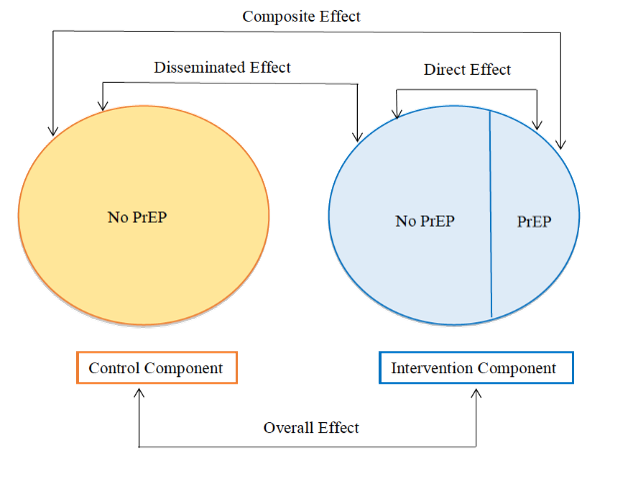
\includegraphics{Figures/figure1.png}
    \caption{The causal effects of interest for PrEP use in a sexual contact network.}
    \label{fig:1}
\end{figure}
The Direct Effect is easier to estimate in a randomized trial or observational setting when the context is fixed for the interference/spillover set. This is because when very few people are exposed, interference is minimized for the direct effect. RTs rely on this fixed context, which can be summarized as ``No one not in the trial is exposed.'' An example is in a typical vaccine trial, where the contrast of interest is that of vaccine vs. no vaccine in a context where trial participants are surrounded by vaccine naïve communities.

The Spillover and Overall Effects are more difficult to estimate in RTs and Observational studies. This is because the context is itself part of the effect definition. More precisely, these can be treated as effect estimand surfaces where the value of the estimand is conditional on a specific interference / contact pattern, rather than effect estimands. The same is true for the individual effect if interference is not minimized.

\section{Question}
The Direct, Spillover, Composite, and Overall Effects all incorporate changes in the contact patterns of the network or network component into their definitions. As such, the central question of this investigation is: ``Does the way that counterfactuals and counterfactual contrasts are simulated affect the causal estimand that can be estimated and/or the assumptions that need to be made in order to get valid estimates of causal effects under interference?''
%need "if so, ..."

\section{Effect Modification Scenarios and Estimands of Interest}
The roles/effects that model components play may vary between different estimands of interest. The following subsections explore the effects of Network Structure/Generation and Treatment Assignment. 

In the following derivations, let $Y$ be the outcome of interest, $a,a*$ be counterfactuals of treatment strategy $A$, and $j$ be an identifier of a network.
\subsection{Effect of Network Structure}
The effect of network structure may depend on the estimand of interest. 

In observational data, we may estimate
\begin{equation}\label{eq:1}
    \mathbb{E}_{i}\left[Y_{i,j}^{a}-Y_{i,j}^{a*}\right],
\end{equation}
the expectation over individuals $i$ within the network $j$. If we have a particular network realization of interest, this comparison is estimating the average effect on that network $j$: 
\begin{equation}\label{eq:2}
    \mathbb{E}\left[Y^{a}-Y^{a*}|j\right],
\end{equation}

In simulated data, we may not be interested in any particular network, so we instead estimate
\begin{equation}\label{eq:3}
    \mathbb{E}\left[Y^{a}-Y^{a*}\right]=\mathbb{E}_{j}\left[\mathbb{E}\left[Y_{j}^{a}-Y_{j}^{a*}\right]\right],
\end{equation}
taking the expectation under treatment over all possible network structures considered. 
\subsubsection{Equivalence of Observational and Simulation Estimands}
We are also interested in determining whether the observational estimand in \ref{eq:1} is equal to the simulation estimand in \ref{eq:2}. If our contact network of interest is drawn at random from a specified distribution, and the true effect is expected to be identical (up to stochasticity) in all such networks, then the effect in any one network should approximate the effect in all networks.

In epidemiological terms: If there is no effect modification by contact network structure, $j$, then we expect that the average effect across contact networks is the same as the average effect on a given contact network, hence the equivalence of \ref{eq:1} and \ref{eq:2}:
\begin{equation}\label{eq:4}
      \mathbb{E}\left[Y_{j}^{a}-Y_{j}^{a*}\right]=\mathbb{E}\left[Y^{a}-Y^{a*}\right]=\mathbb{E}_{j}\left[\mathbb{E}\left[Y_{j}^{a}-Y_{j}^{a*}\right]\right].
\end{equation}
\subsection{Effect of Treatment Assignment}
We are usually interested in treating only a subset of eligible individuals. Specifically, we want to prioritize those individuals who have at least one infectious contact. However, it is generally impossible to identify all such individuals. As such, the estimand must aggregate all possible treatment distributions and account for the heterogeneity of the treatment effect between those with and without infectious contacts.

Thus, while we are interested in estimating \ref{eq:1} from observational data, we actually interested estimating 
\begin{equation}\label{eq:5}
    \mathbb{E}_{\Set{a,a*   }}\left[\mathbb{E}\left[Y_{j}^{a}-Y_{j}^{a*}\right]\right],
\end{equation}
averaging over all ways that a treatment $A$ can applied to network $j$. That is, we take expectations over all individuals in a given network $j$, then over all treatments $a,a*$ of $A$ that can be applied to the network.

The estimand in \ref{eq:3} is also of interest in a simulation model since we don't preferentially apply either value of $A$. Simulation studies theoretically avoid the limiting assumption that the observed treatment scenario is representative by allowing for all possible combinations to be simulated. However, in practice the number of combinations is large and exhaustive simulation is computationally impractical.


For a single time point, let $N$ denote the number of uninfected individuals in the network, and $k <N$ denote the number of individuals in the network who will receive treatment. Then, there are $\binom{N}{k}$ unique network configurations.

Assume that $k$ is chosen at random from the $N$ uninfected individuals, and that $n<N$ of the uninfected individuals have an infectious contact. The expected number of unique network configurations  in which all treated individuals have no infectious contacts (and thus a contribution of 0 to the effect estimate) is then given by $\binom{N-n}{k}$. Then, the proportion of network configurations in which at least one treated individual has at least one infectious contact is 
\begin{equation}\label{eq:6}
    \frac{{\binom{N}{k}}-{\binom{N-n}{k}}}{{\binom{N}{k}}}=1-\left(1-\frac{k}{N}\right)^{n}.
\end{equation}
That is, the probability of at least one node $i$ assigned to treatment with at least one infectious contact for a given network structure $j$ and treatment assignment is:
\begin{equation}\label{eq:7}
    P \coloneqq \mathbb{P}\left(n_{i}=1 \vert k_{i}=1,j,a,a*\right)=1-\left(1-\frac{k}{N}\right)^{n}.
\end{equation}
Note that 
\begin{equation}\label{eq:8}
    \lim_{N \to \infty}P=\begin{cases}0 & k,n \text{ fixed} \\ 1 & k \to N \lor n \to N  \end{cases}
\end{equation}

\subsection{Effect of Network Regeneration}
It is important to note that we often do not actually estimate \ref{eq:2}. If we are regenerating the network at each iteration of the simulation, then we are estimating \begin{equation}\label{eq:9}
    \mathbb{E}_{\Set{j,j*}}\left[\mathbb{E}\left[Y_{j}^{a}\right]-\mathbb{E}\left[Y_{j*}^{a*}\right]\right],
\end{equation} 
which is the average over the joint distribution of all combinations of network structures $j$ and $j*$ of the difference between the average potential outcome under treatment assignment $a$ with network structure $j$ and the average potential outcome under  treatment assignment $a*$ with network structure $j*$.

This raises the question of whether the network regeneration estimand in \ref{eq:8}  is equal to the network structure estimand from \ref{eq:2}. Recall that causal contrasts require that the counterfactuals being compared represent 2 possible counterfactual experiences of a single group. As such, if we are regenerating the network each time that we generate a counterfactual, then we need to assume that every network instance and every treatment represents a possible experience of the exact same individuals. 

But, in some networks an individual might be treated and have an infectious contact, while in others they may be treated and not have an infectious contact, or not be treated and have an infectious contact, or be treated and have no infectious contacts. If we did not explicitly average over all of these scenarios, we would need to assume constancy of counterfactuals across networks in addition to constancy of effects across networks. This is tantamount to assuming no effect modification for all possible treatment values, which requires no confounders of outcome by contact pattern or treatment.
%Mention randomization!
\subsubsection{A Note on Some Problems and Assumptions}

However, it is important to remember that the utility of modelling effects on networks comes from the ability to encode network structure/contact patterns as effect modifiers. In this particular context, not assigning treatment based on contact risk means that contact risk strongly affects infection risk. Also, assignment by contact risk would still allow for effect modification if limitations in identifying future contacts occur. Since it is often nearly impossible to perfectly identify future infectious contacts in advance, contact risk effect modification will occur whether or not treatment is applied.

A key assumption to keep in mind is that lack of effect modification requires that the effect estimate does not depend on who in each community does/does not get exposed. But, we know that there is heterogeneity in real contact patterns, and that Independence between contact patterns and exposure status does not usually hold. In particular, individuals usually choose exposure on the basis of perceived outcome risk. As such, the individual-level benefit of receiving a protective exposure will depend on whether that individual receives an infectious exposure. Thus, individual effects are not homogeneous and we must consider infectious exposure an effect modifier. Individual beliefs about the likelihood of an infectious exposure will also cause both infectious and protective exposures. Thus, infectious exposure is thus both a confounder and an effect modifier for the individual effect and this propagates to the overall effect. 
\subsubsection{Equivalence of Network Regeneration and Simulation Estimands}
We are then interested in whether the estimands in \ref{eq:8} and \ref{eq:2} are equivalent.

Having identified that the network structure $j$ is an effect modifier, we know it is possible that \begin{equation}
    \mathbb{E}_{j}\left[\mathbb{E}\left[Y_{j}^{a}-Y_{j}^{a*}\right]\right] \neq \mathbb{E}\left[Y_{j}^{a}-Y_{j}^{a*}\right],
\end{equation}
and that
\begin{equation}
    \mathbb{E}_{j}\left[\mathbb{E}\left[Y_{j}^{a}-Y_{j}^{a*}\right]\right]\neq  \mathbb{E}_{\Set{j,j*}}\left[\mathbb{E}\left[Y_{j}^{a}\right]-\mathbb{E}\left[Y_{j*}^{a*}\right]\right]. 
\end{equation}

But our analyses estimate either 
\begin{equation*}
\mathbb{E}\left[Y_{j}^{a}-Y_{j}^{a*}\right]    
\end{equation*}
or 
\begin{equation*}
    \mathbb{E}\left[Y_{j}^{a}\right]-\mathbb{E}\left[Y_{j*}^{a*}\right]
\end{equation*}
and then combine them across all runs.
\section{Goal}
An important goal of this investigation is then to identify valid approaches and assumptions for estimating $$\mathbb{E}\left[Y^{a}-Y^{a*}\right]$$.

We first need to develop estimators and clarify the assumptions for identifying each of the expectations $$\mathbb{E}_{\Set{j,j*}}\left[\mathbb{E}\left[Y_{j}^{a}\right]-\mathbb{E}\left[Y_{j*}^{a*}\right]\right],$$ and
$$\mathbb{E}_{j}\left[\mathbb{E}\left[Y_{j}^{a}-Y_{j}^{a*}\right]\right]$$ expanding on the definitions of overall, composite, direct, and spillover effects.

We then create a simulated network with known effects.

Finally, we draw model parameters from that network and obtain estimates using standard methods (and any additional methods identified in the first step.
\section{Illustrative Example}
\subsection{Control Scenario}
\begin{figure}[H]
    \centering
    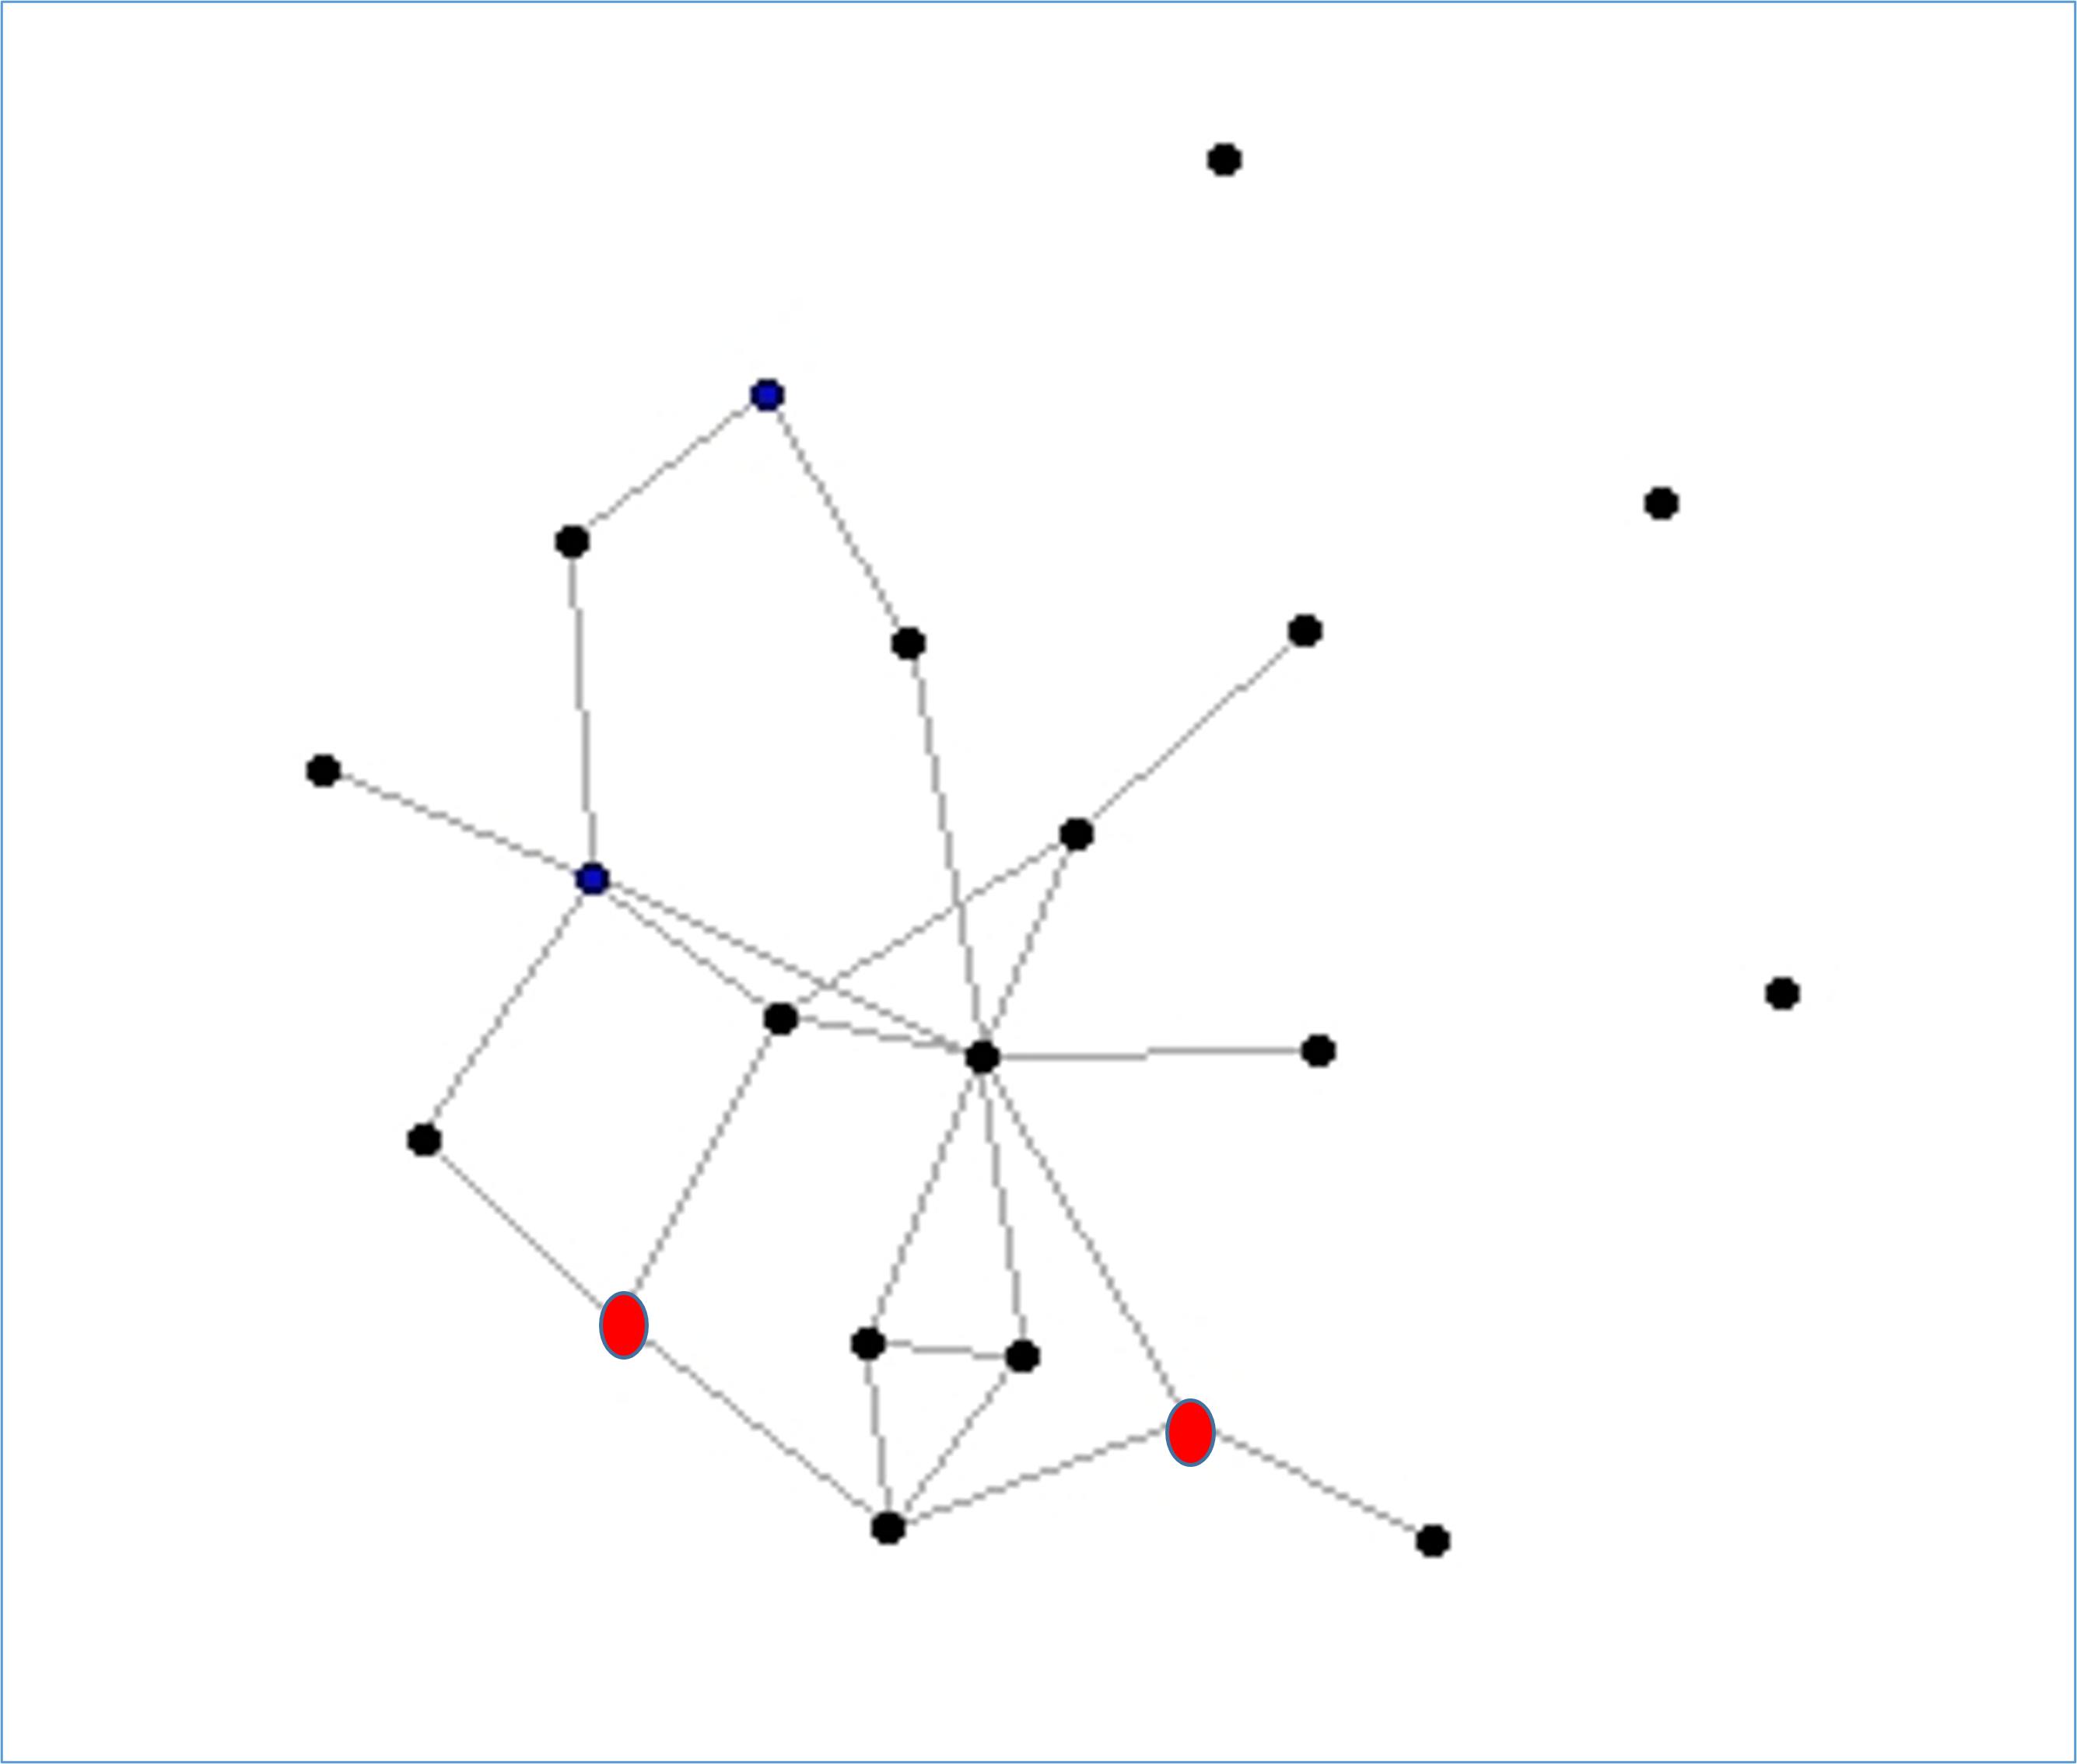
\includegraphics[scale=0.5]{Figures/Network Example 1.png}
    \caption{Control data generated for network example. 2 red nodes represent HIV positive individuals. 18 black nodes represent uninfected individuals.}
    \label{fig: Figure 2}
\end{figure}
Consider the control network in Figure \ref{fig: Figure 2}  above with 20 nodes and a probability of HIV infection of 10\%. If we want to estimate the Overall Effect of 20\% PrEP use vs. 10\% PrEP use, we assume: HIV status is known and PrEP not assigned to PHIV; PrEP is assigned to individuals without HIV at random; Single time-step iterations in the simulation to minimize interference.

 Of the 18 uninfected individuals (black nodes), 5 have an infectious contact. 13 individuals are uninfected with no infectious contacts.
\begin{figure}[H]
    \centering
    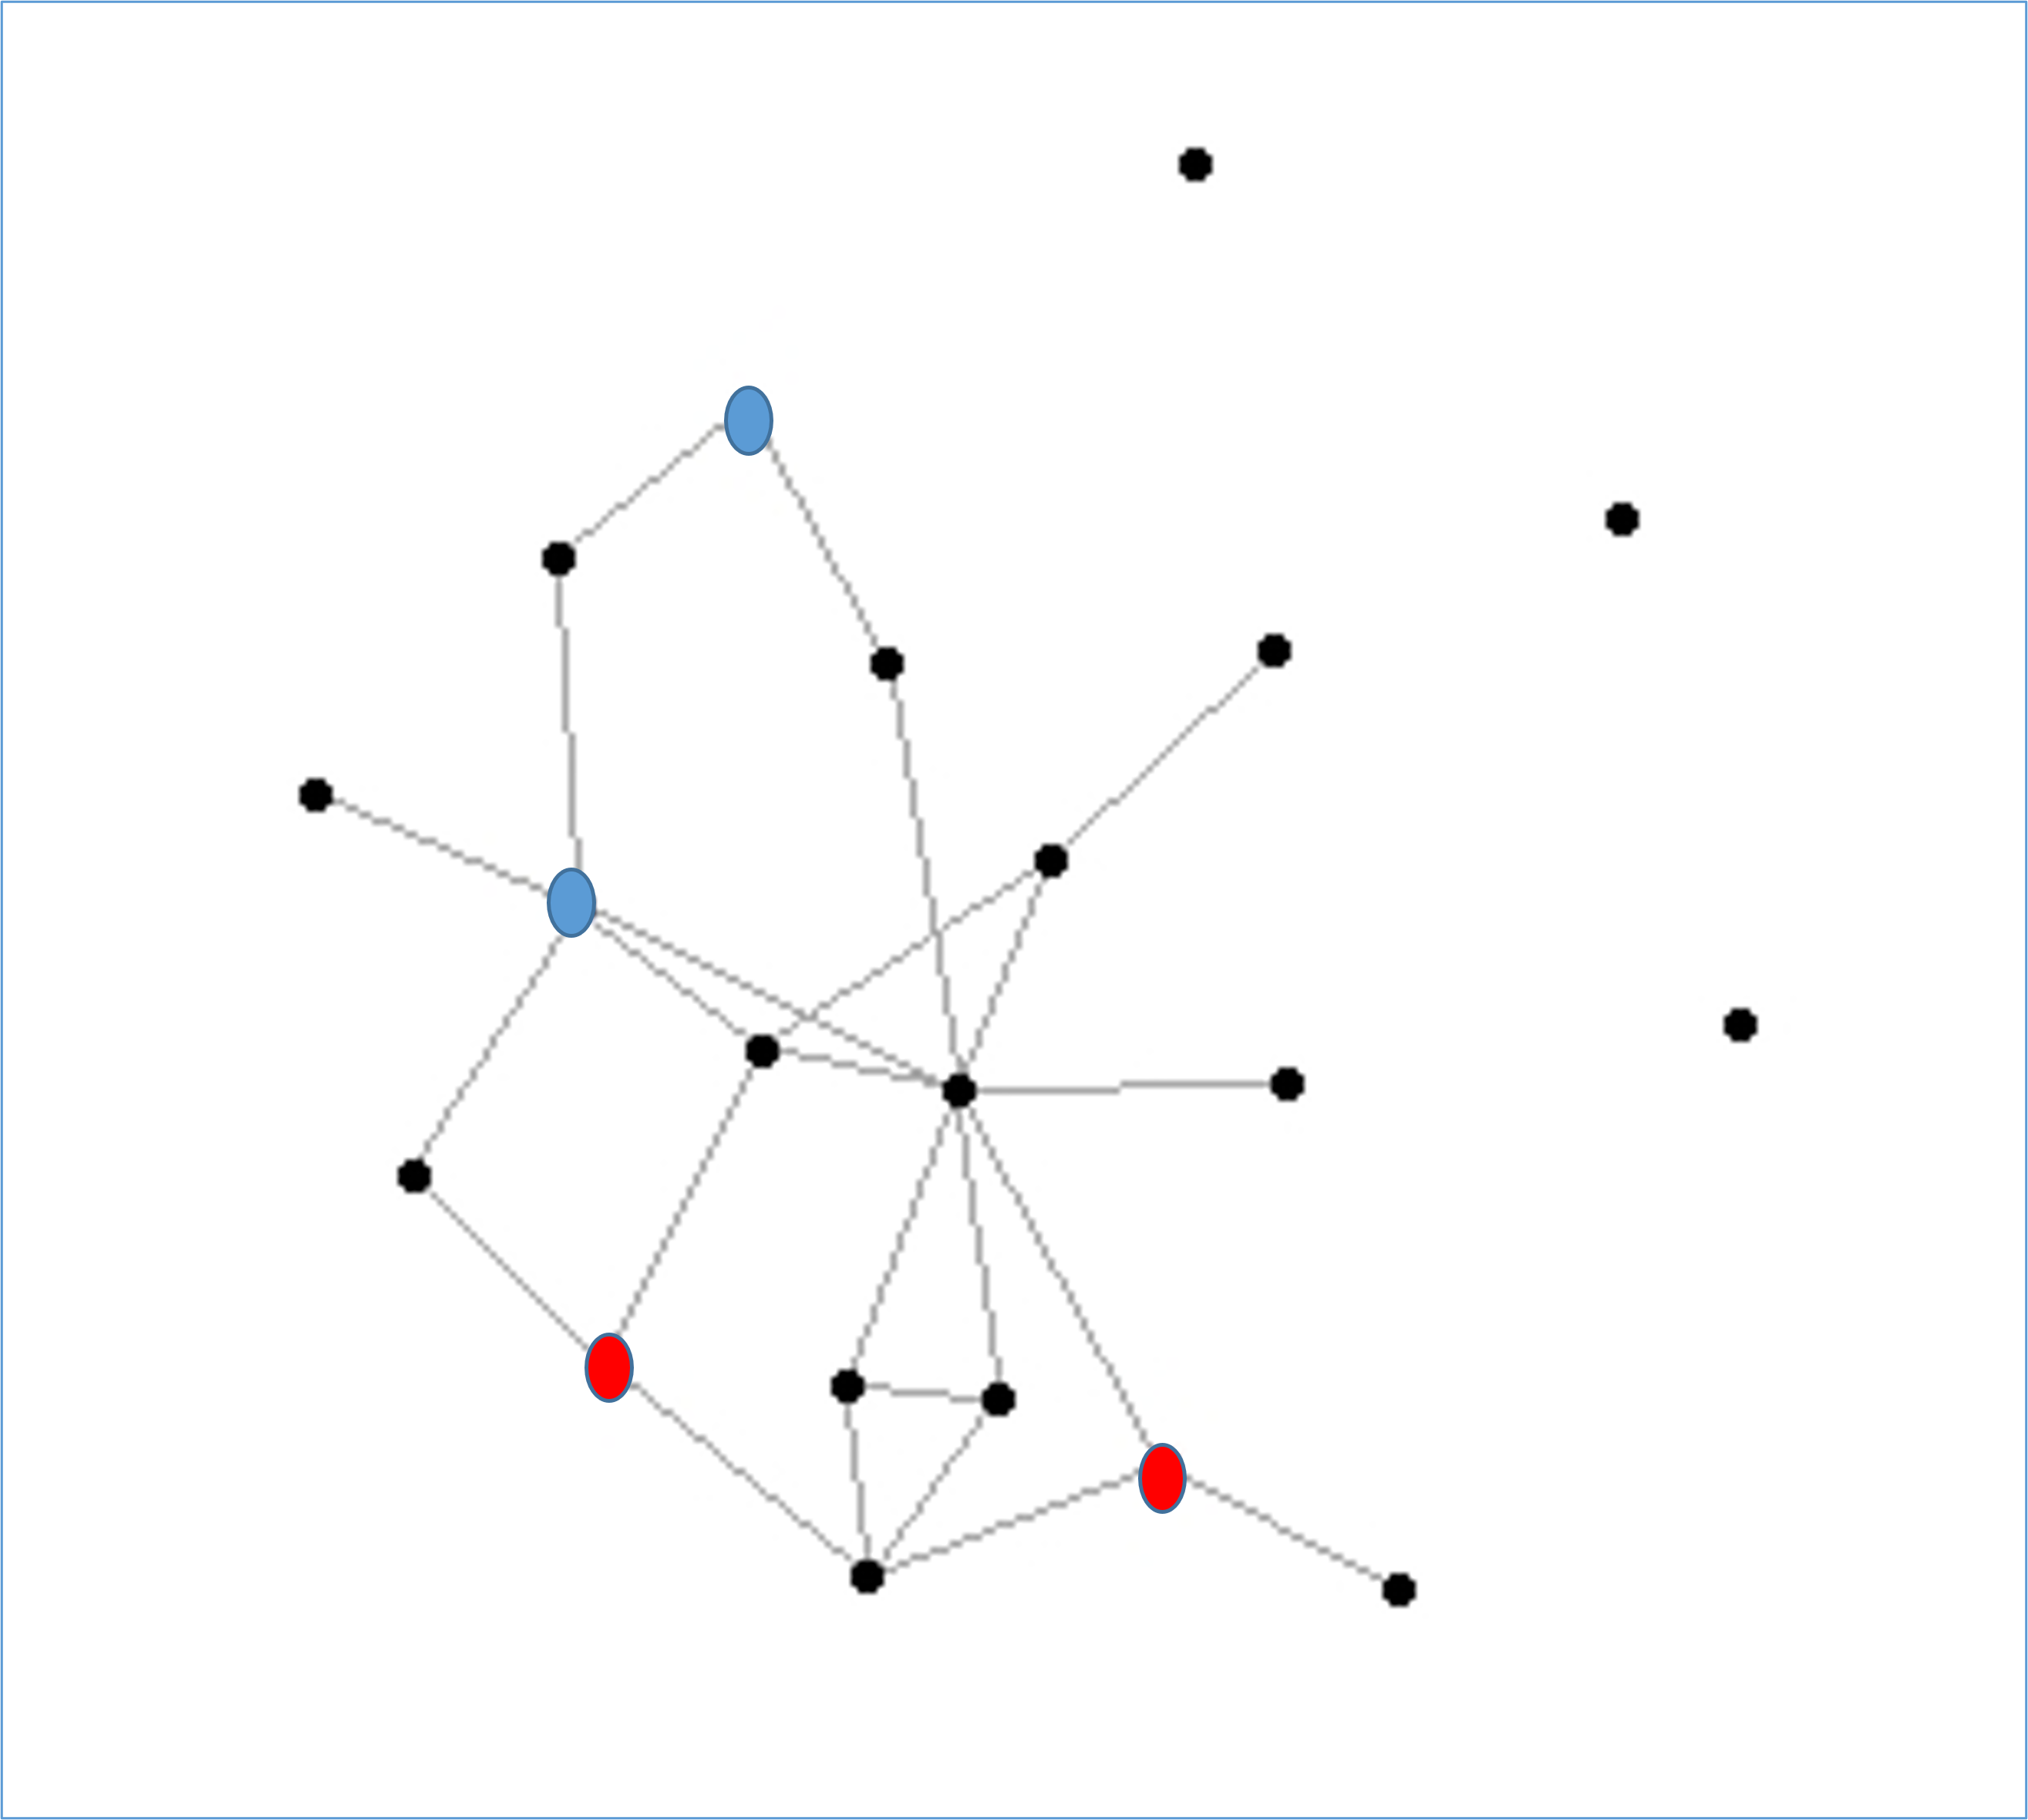
\includegraphics[scale=0.5]{Figures/Network Example 2.png}
    \caption{Random PrEP assignment to the network with 10\% coverage of uninfected individuals. 2 blue nodes represent uninfected individuals assigned to PrEP.}
    \label{fig:Figure 3}
\end{figure}

After PrEP assignment in Figure \ref{fig:Figure 3}. We can then compute probabilities of being infected given PrEP Assignment. Notice that neither of the 2 individuals assigned to PrEP are among the 5 uninfected individuals with known infectious contacts, so $$\mathbb{P}\left(\text{HIV}\vert \text{PrEP}\right)=\left(\frac{2}{2}\right)0=0.$$
Likewise, there are 16 uninfected individuals who were not assigned to PrEP, of whom 5 have an infectious contact. Let $p_{1}=\mathbb{P}\left(\text{HIV} \vert \text{infectious contact} \cap \text{PrEP}^{c}\right)$ denote the probability of HIV infection given at least one infectious contact and not being assigned to PrEP.  Then, $$\mathbb{P}\left(\text{HIV} \vert \text{PrEP}^c\right)=\frac{5}{16}p_{1}+\left(\frac{11}{16}\right)0=\frac{5}{16}p_{1}.$$ Note, there is no HIV risk for those without infectious contacts.
\subsection{Treatment Scenario 1} 
\begin{figure}[H]
    \centering
    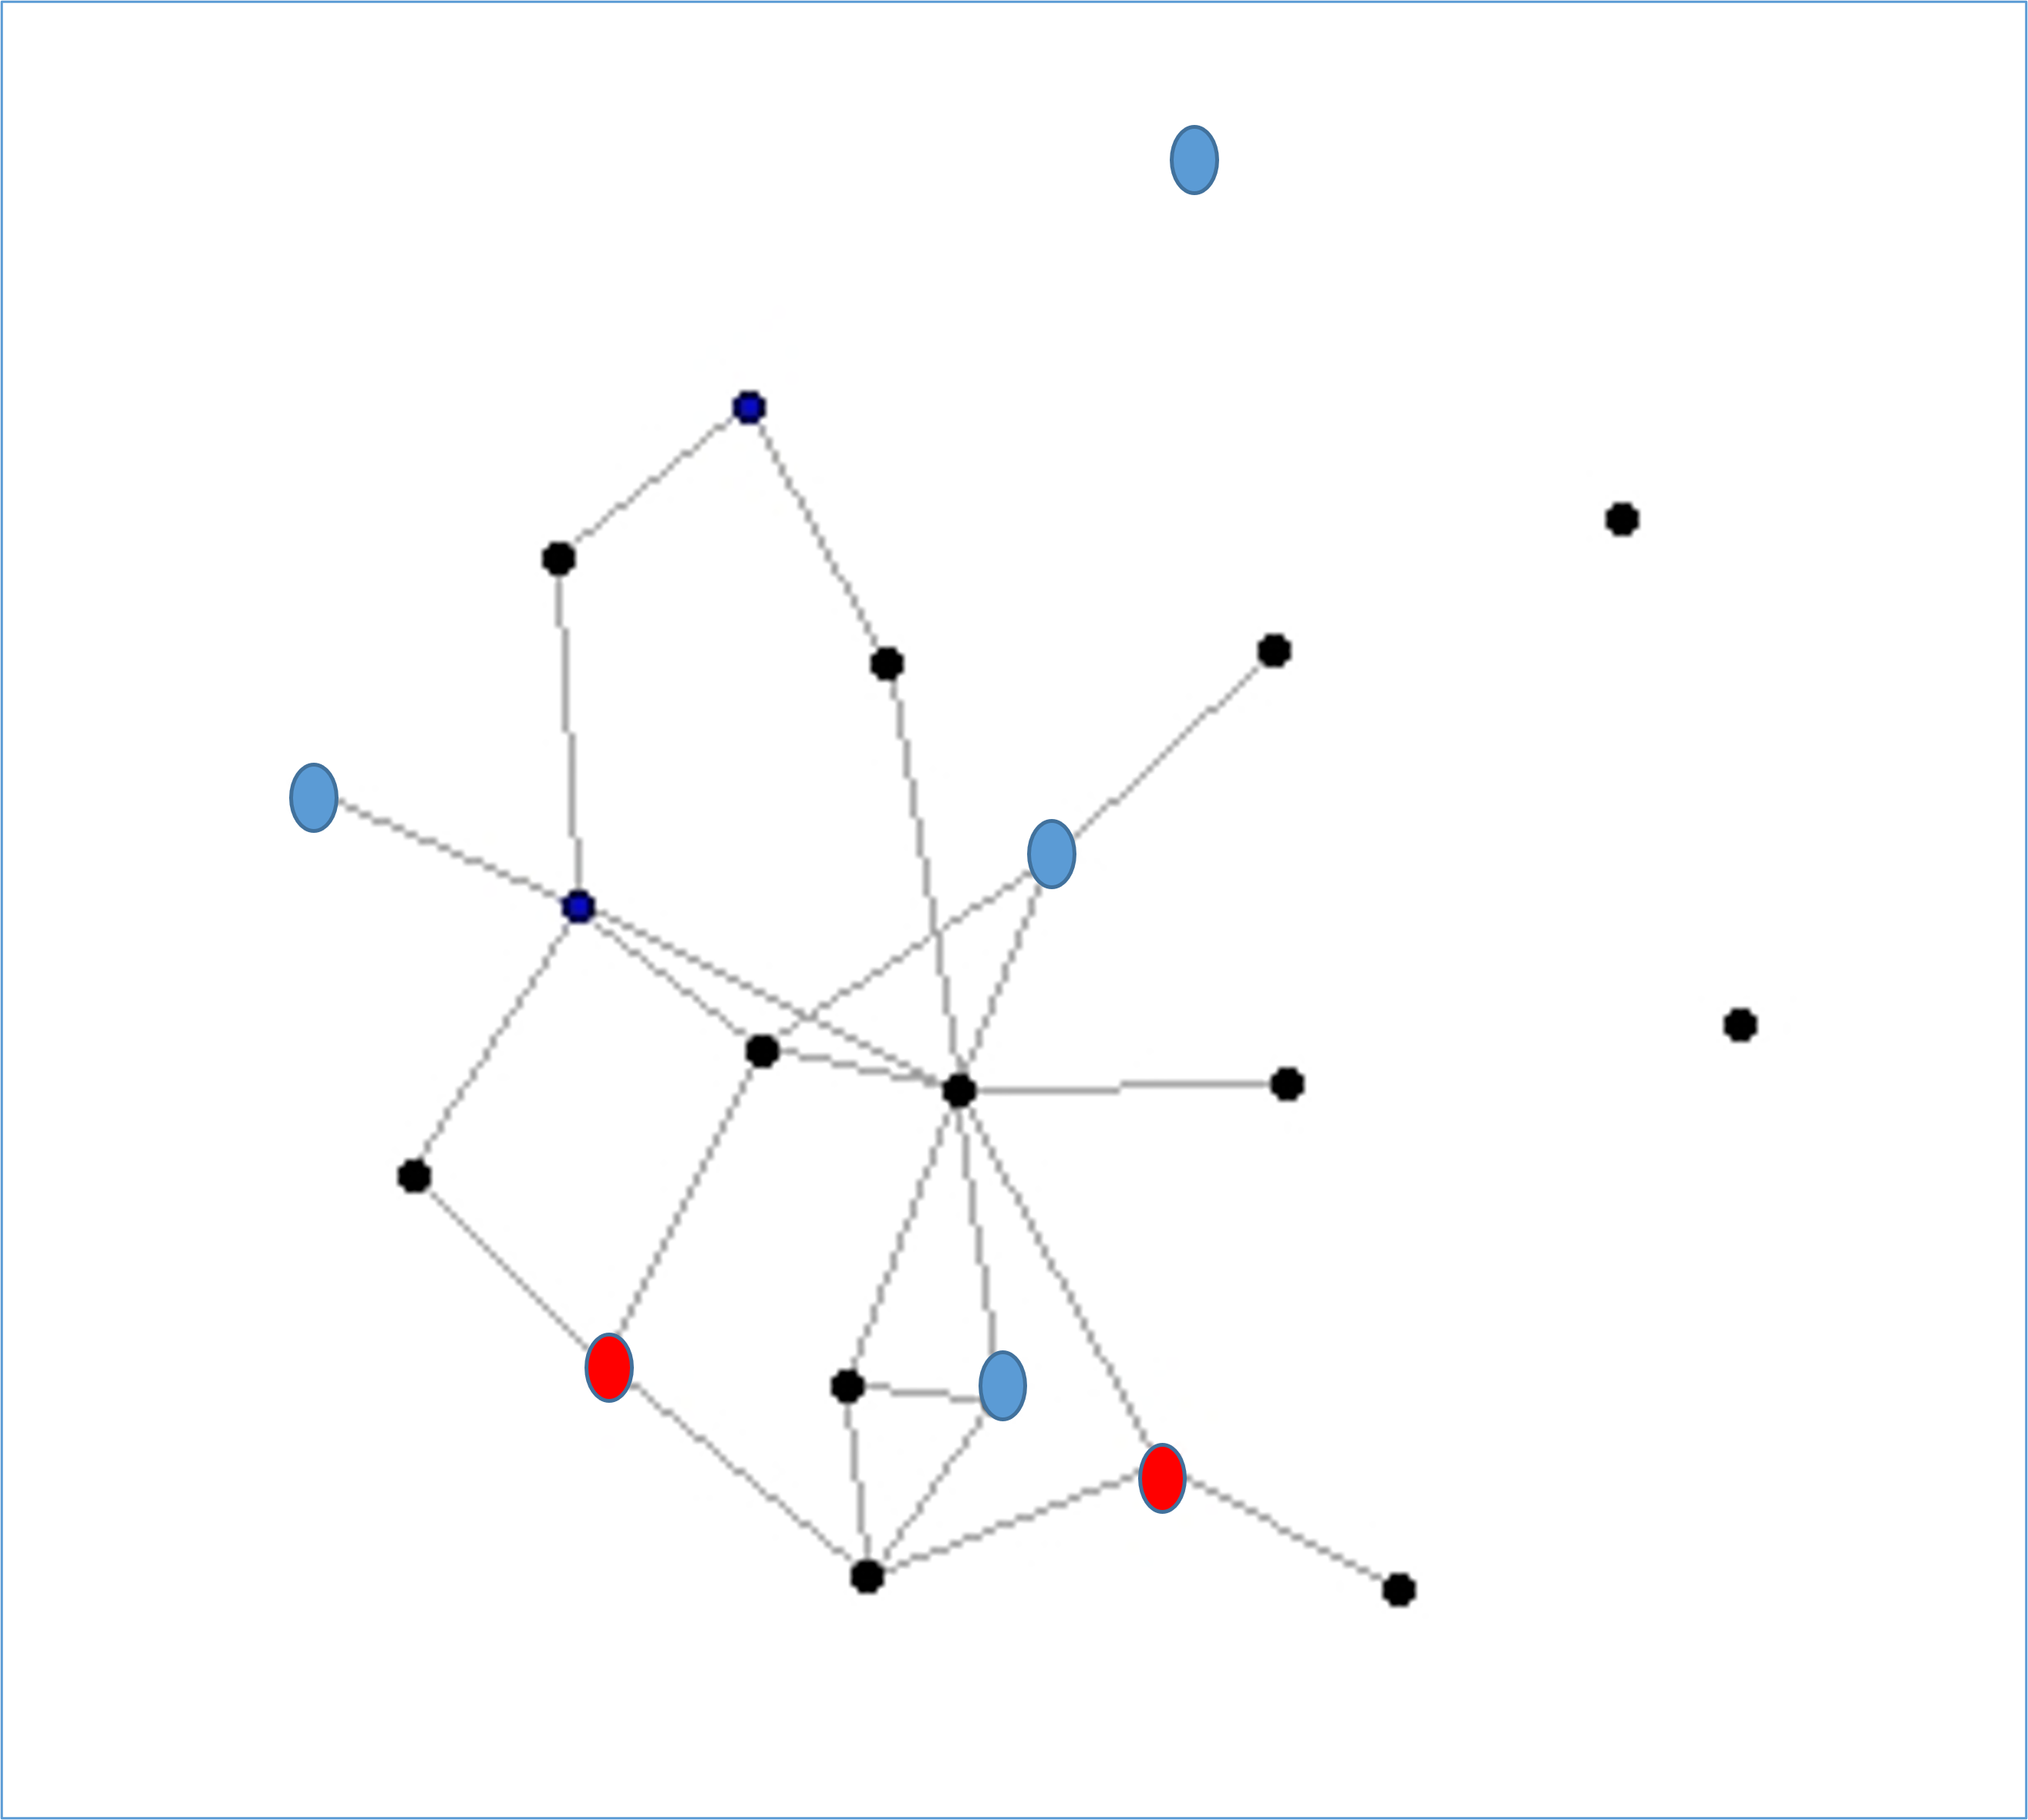
\includegraphics[scale=0.5]{Figures/Network Example 3.png}
    \caption{Treatment Option 1: Randomly assigned 20 \% coverage (blue nodes) to the uninfected individuals.}
    \label{fig:Figure 4}
\end{figure}

One option is to randomly assign 20 \% PrEP coverage to uninfected individuals, as in Figure \ref{fig:Figure 4} above.
We can see that 4 uninfected individuals were assigned to PrEP, but none of these have an infectious contact. So, $$\mathbb{P}\left[\text{HIV}\vert \text{PrEP} \right]=0.$$ Likewise, there are 14 uninfected individuals in the network who have been assigned no PrEP, 5 of whom have an infectious contact. Thus, $$\mathbb{P}\left[\text{HIV} \vert \text{ PrEP}^{c}\right]=\frac{5}{14}p_{1}+\frac{9}{14}\left(0\right).$$  

\subsection{Treatment Scenario 2} 
\begin{figure}[H]
    \centering
    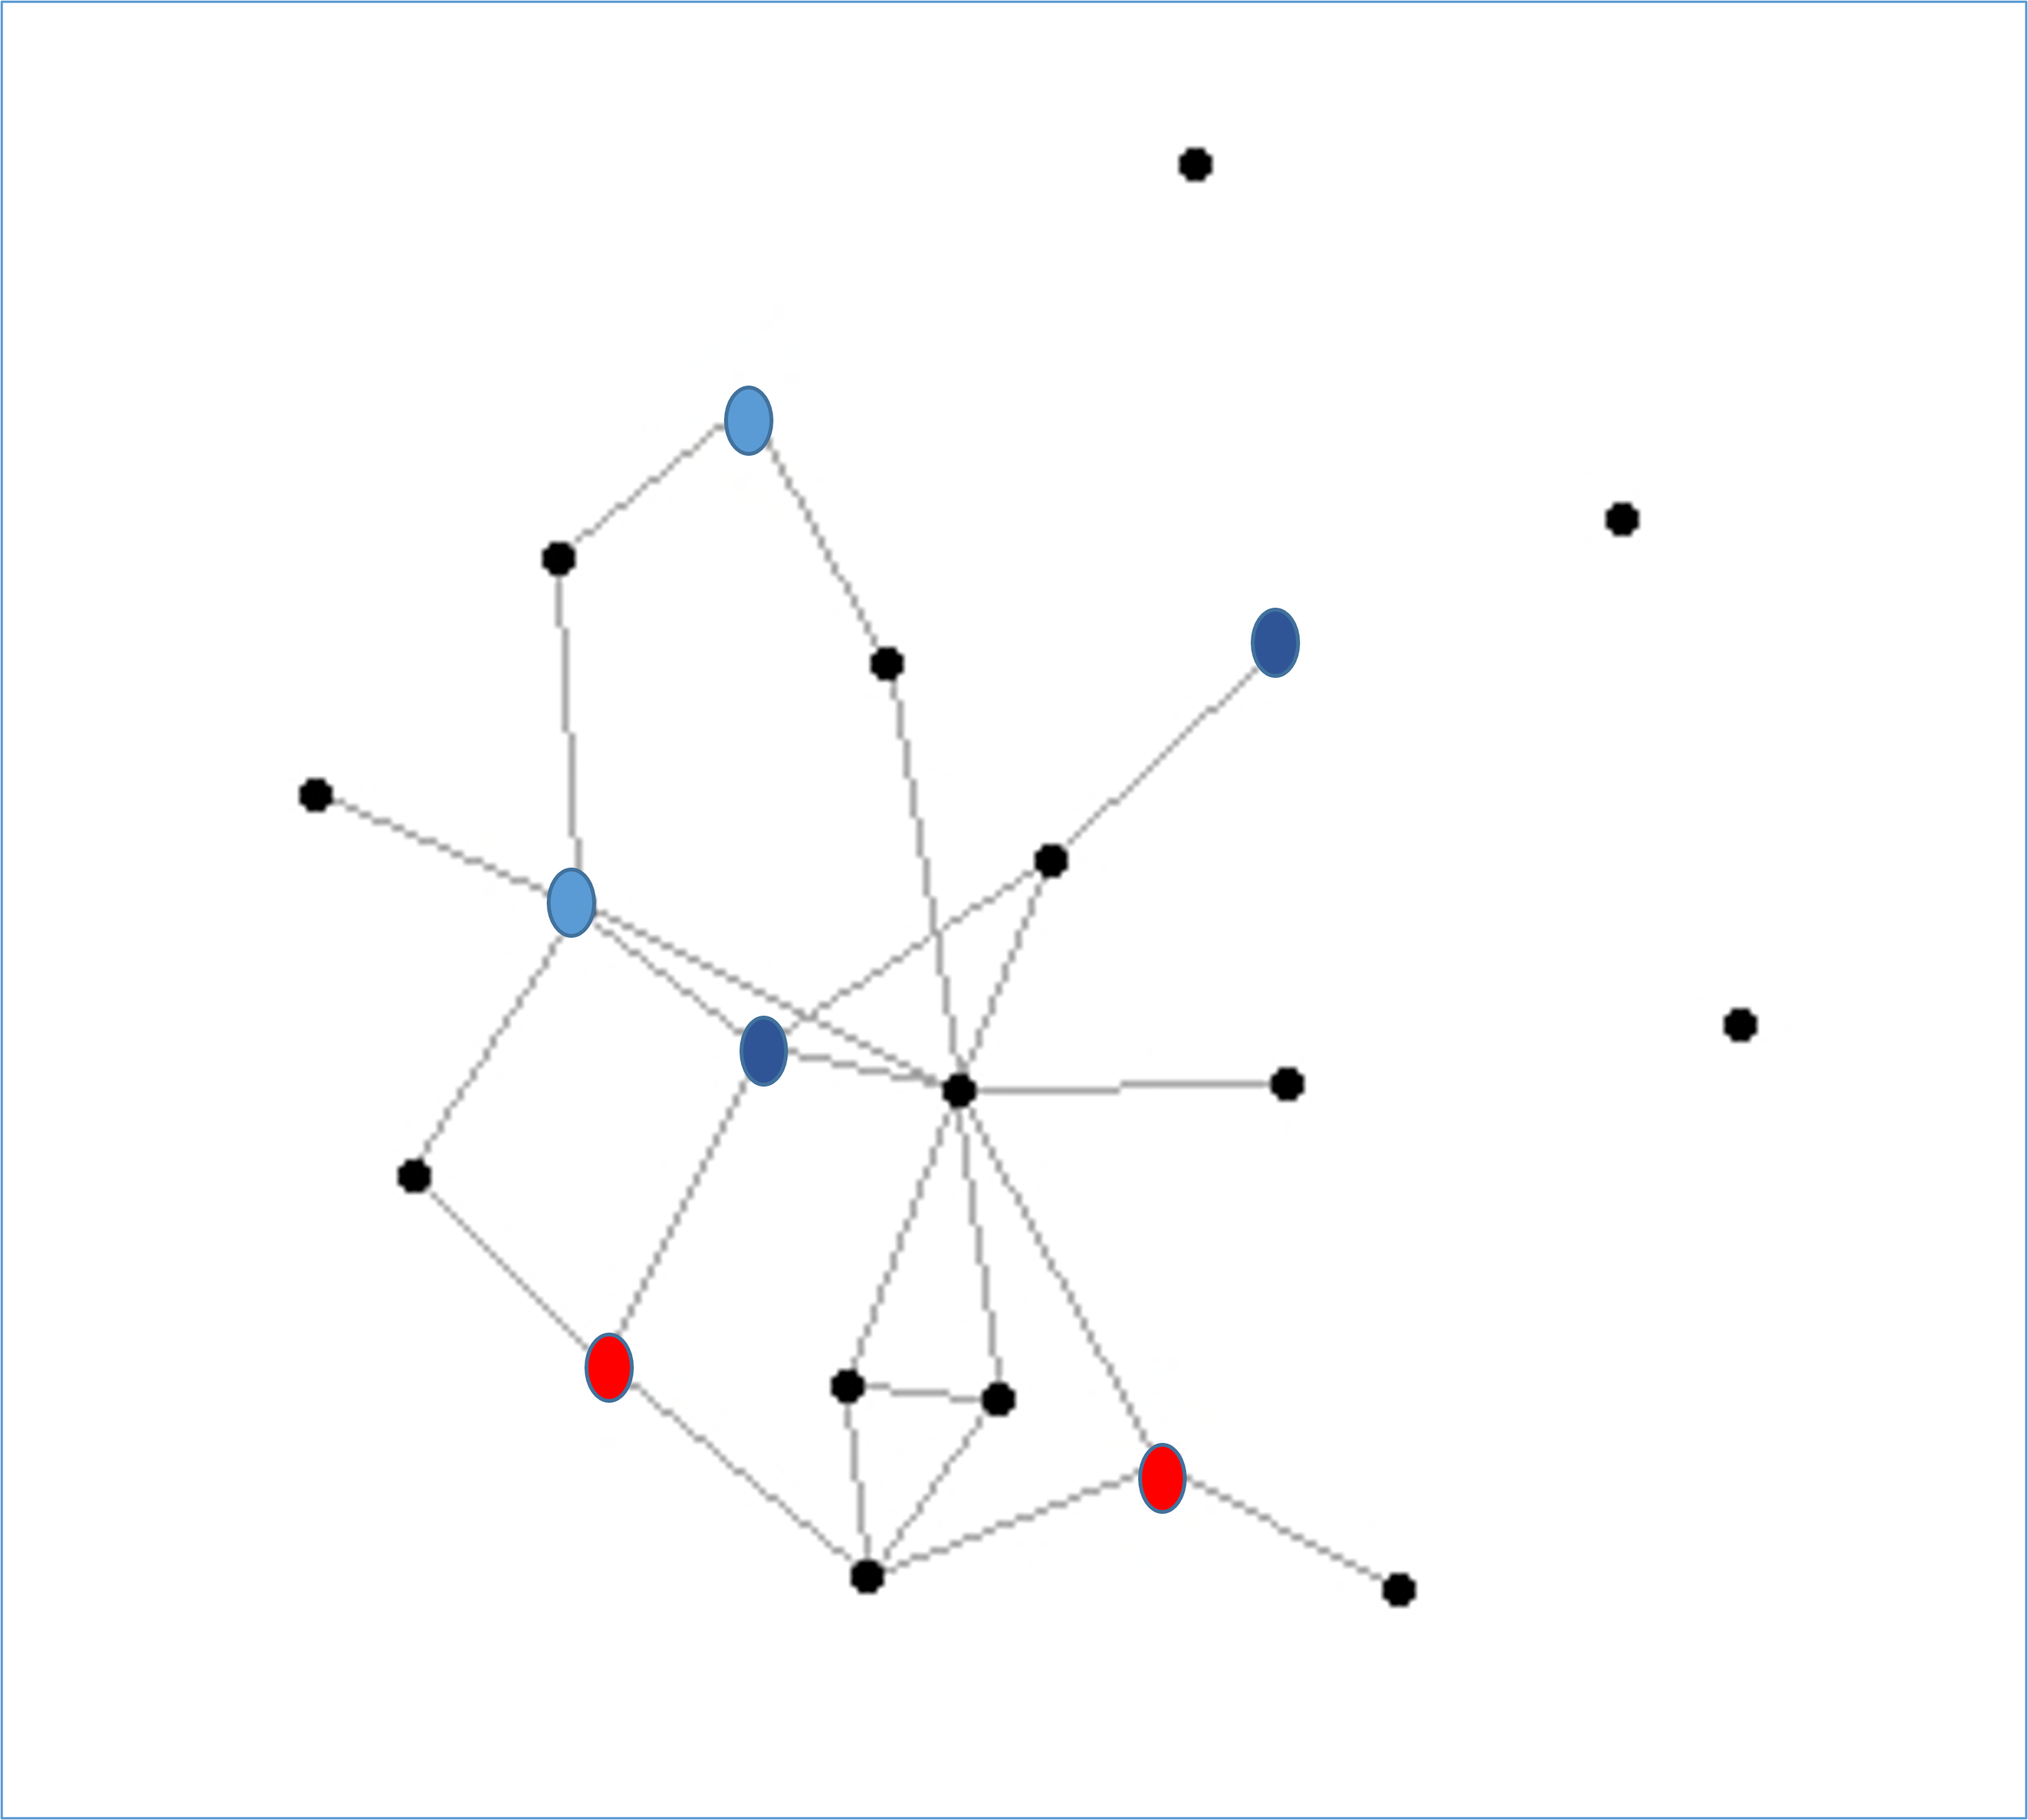
\includegraphics[scale=0.5]{Figures/Network Example 4.png}
    \caption{Treatment Option 2: Randomly assign an additional 10\% PrEP coverage to the Control Scenario network for a total coverage of 20\%. 2 uninfected individuals from the control scenario (light blue nodes) were assigned PrEP. 2 additional uninfected individuals (dark blue nodes) were assigned PrEP. }
    \label{fig:Figure 5}
\end{figure}

Another option is to assign PrEP coverage to an additional 10 \% remaining uninfected individuals from the control scenario. See Figure \ref{fig:Figure 5} above. 
We can see that 2 uninfected individuals have been assigned to PrEP, neither of whom have an infectious contact. 2 additional uninfected individuals were assigned PrEP, one of whom has an infectious contact. Let $p_{2}=\mathbb{P}\left[\text{HIV } \vert \text{ infectious contact} \cap \text{PrEP}\right].$ Then, $$\mathbb{P}\left[\text{HIV } \vert \text{ PrEP}\right]=\frac{1}{4}p_{2}+\frac{3}{4}\left(0\right).$$  
14 uninfected individuals have been assigned no PrEP, 5 of whom have an infectious contact. So, $$\mathbb{P}\left[\text{HIV } \vert \text{ PrEP}^{c}\right]=\frac{5}{14}p_{1}+\frac{9}{14}\left(0\right).$$
\subsection{Treatment Scenario 3}
\begin{figure}[H]
    \centering
    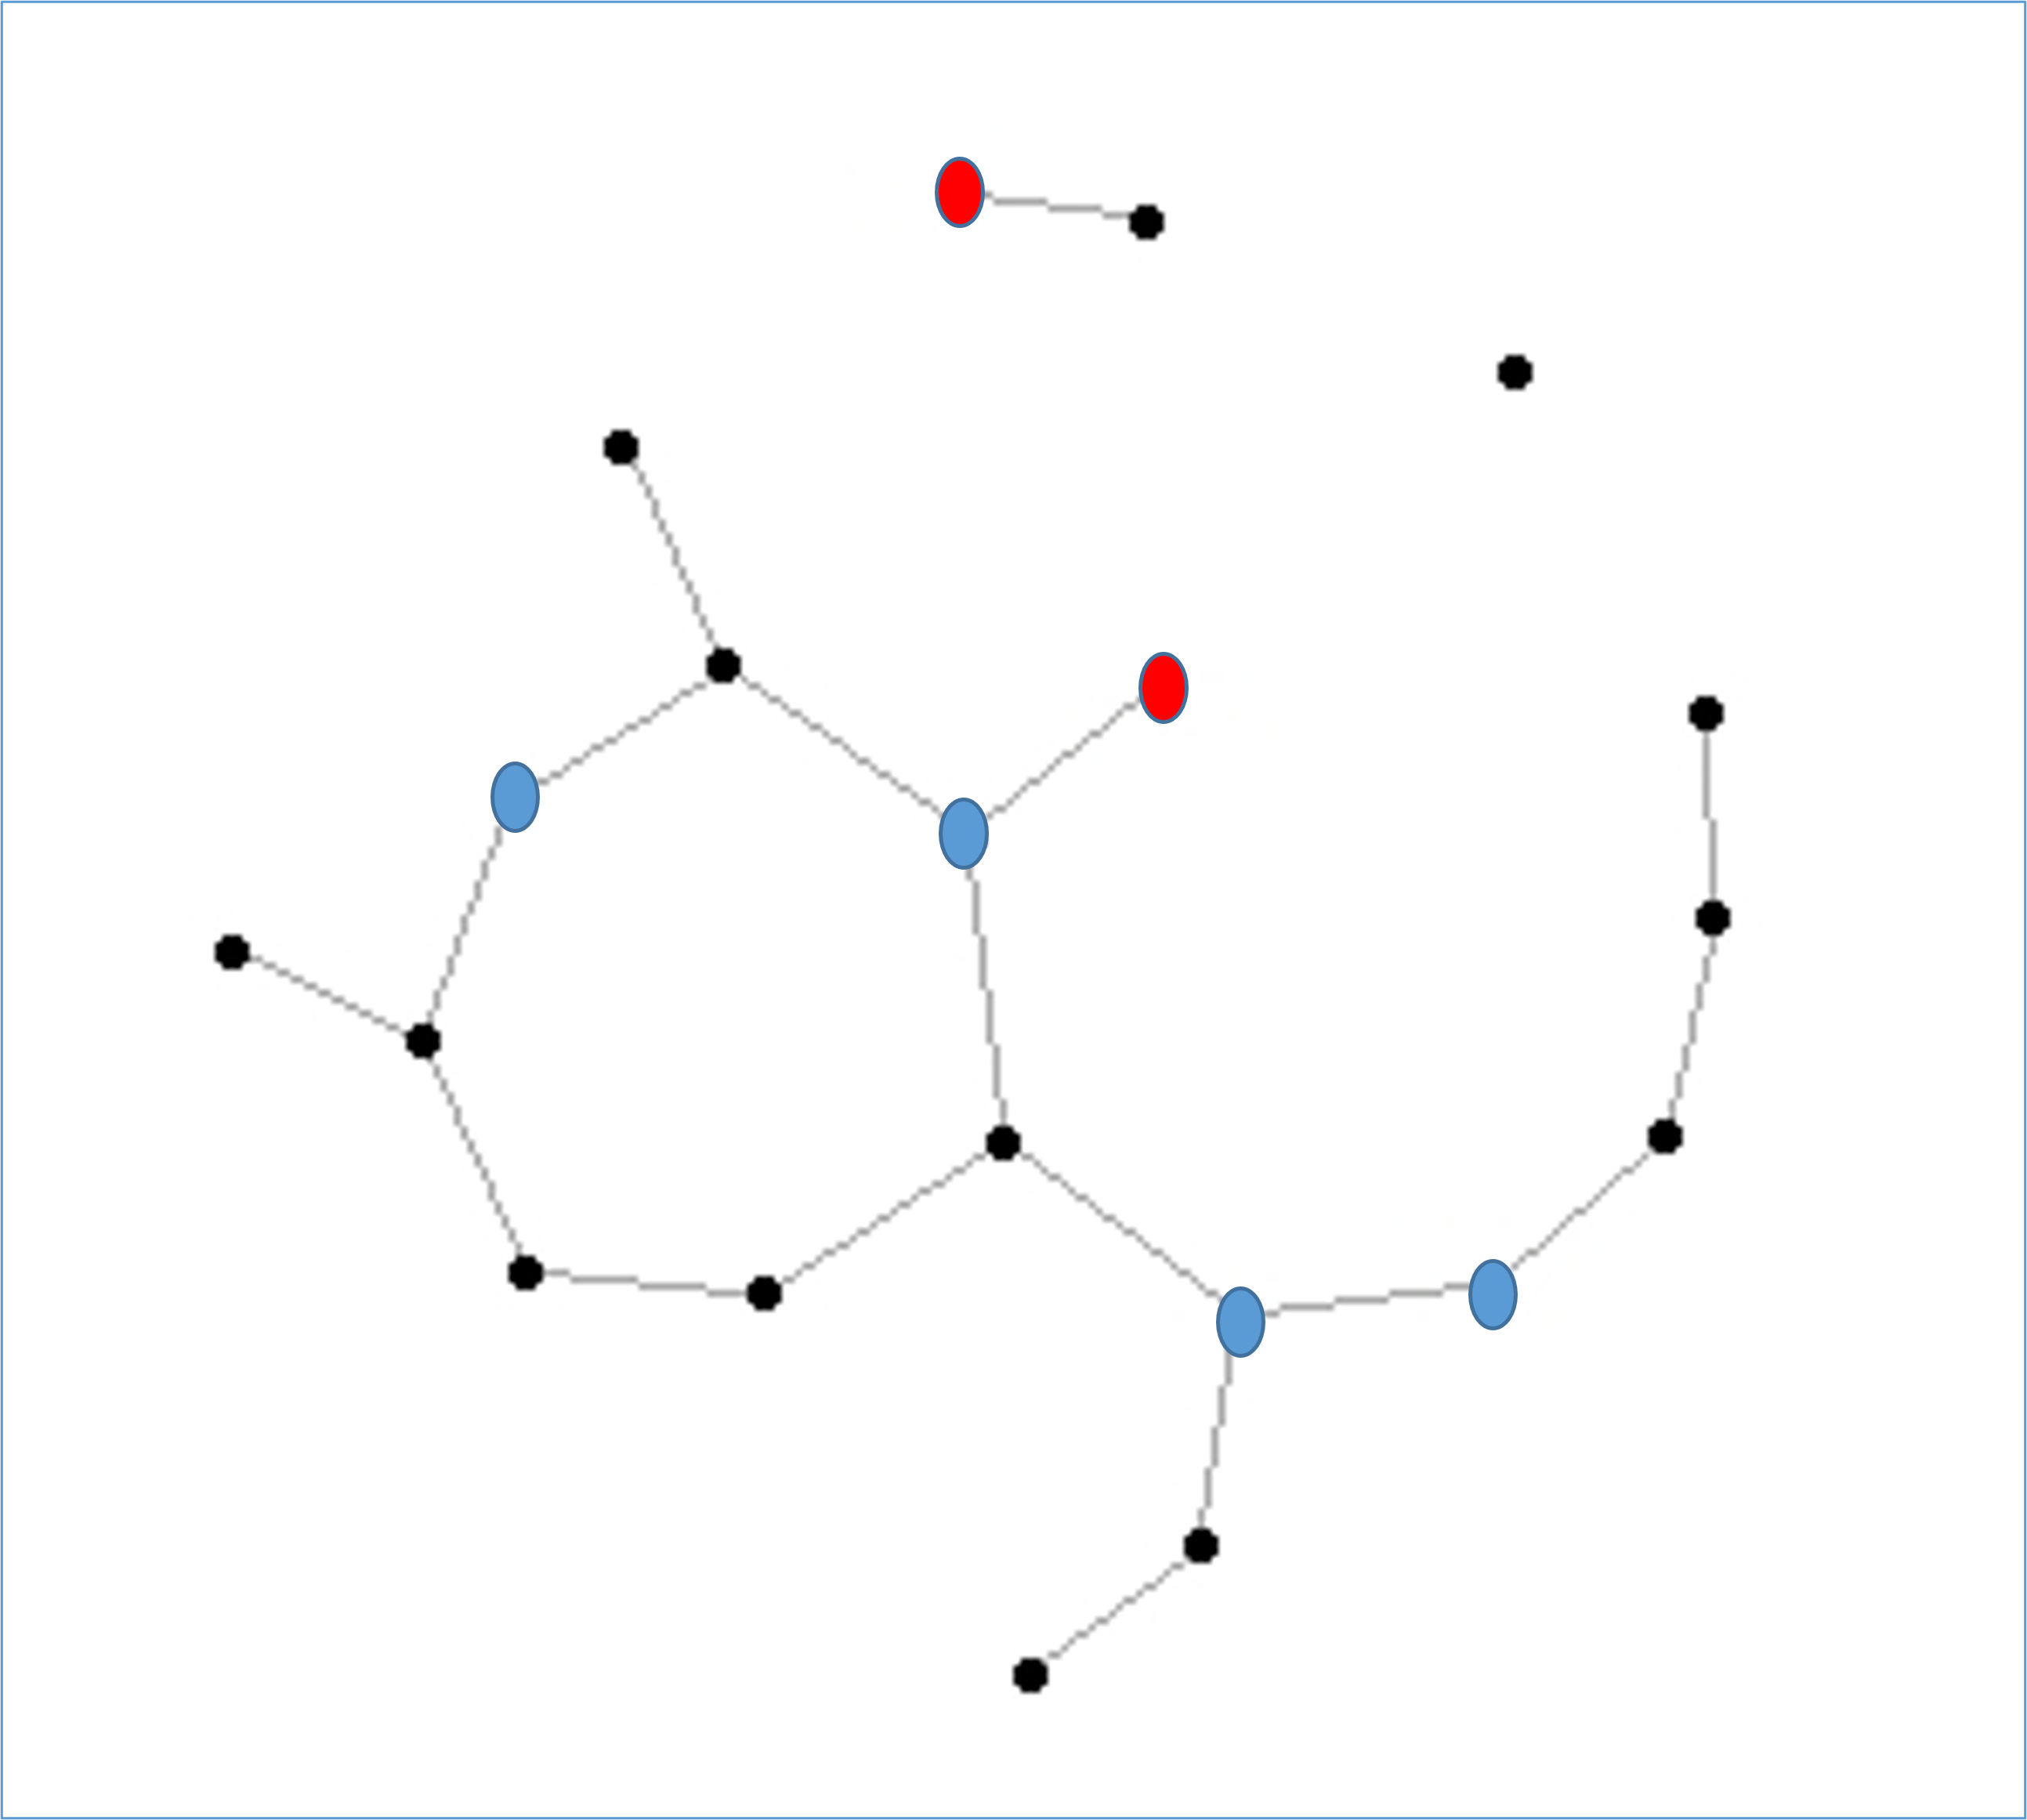
\includegraphics[scale=0.5]{Figures/Network Example 5.png}
    \caption{Treatment Option 3: Re-generate the network and randomly assign 20 \% PrEP coverage. 2 individuals are infected (red nodes). There are 4 uninfected individuals assigned to PrEP (light blue nodes), of whom one has an infectious contact. }
    \label{fig:Figure 6}
\end{figure}

Yet another option is to regenerate the network and randomly assign 20 \% PrEP coverage. See Figure \ref{fig:Figure 6} above. There are 2 infected individuals and 18 uninfected individuals. 2 uninfected individuals have infectious contacts. 4 uninfected individuals have been assigned to PrEP, one of whom has an infectious contact. Thus, $$\mathbb{P}\left[\text{HIV } \vert \text{PrEP}\right]=\frac{1}{4}p_{2}+\frac{3}{4}\left(0\right).$$
There are 14 uninfected individuals who have been assigned no PrEP, one of whom has an infectious contact. Hence, $$\mathbb{P}\left[\text{HIV } \vert \text{ PrEP}^{c}\right]=\frac{1}{14}p_{1}+\frac{13}{14}\left(0\right).$$
\subsection{Effect Estimates}
We can now compute and compare the effect of 20\% PrEP coverage vs. 10\% PrEP coverage for each of the 3 scenarios.
\begin{center}
    \begin{tabular}{|c|c|c|}
    \hline
    PrEP Assignment Scenario     & $\mathbb{P}\left[\text{HIV} \vert \text{PrEP}\right]$ &  Effect Estimate  \\
         \hline
      10 \% Control   & $\frac{5}{18}p_{1}$ & NA\\
      \hline
      20\% random assignment on control network & $\frac{5}{18}p_{1}$ & 0 \\
      \hline
      20 \% from random additional 10\% on control network & $\frac{1}{18}p_{2}+\frac{5}{18}p_{1}$ & $\frac{1}{18}p_{2}$\\
      \hline
      20 \% random assignment on regenerated network & $\frac{1}{18}\left[p_{1}+p_{2}\right]$ & $\frac{1}{18}p_{2}-\frac{4}{18}p_{1}$\\
      \hline                 
    \end{tabular}                                      \end{center}
\section{Simulation Methods}
Simulations were implemented in R 4.2.1. All code and figure files are available in the GitHub repository: \href{https://github.com/nico-dangelo/Network-Spillover}{Network Spillover}\footnote{https://github.com/nico-dangelo/Network-Spillover}.
Erdős–Rényi random  network graphs for each scenario were generated using igraph version 1.3.2
\subsection{Contrast Estimation}

\section{Results}
\subsection{Erdős–Rényi  Random Graph Models}
We now display simulation results for various parameter combinations in the Erdős–Rényi Random Graph Model.
\begin{center}
    \begin{tabular}{|c|c|c|}
    \hline
         Parameter & Default Value & Range Considered  \\
         \hline
         Network size $N$& 20 & $\Set{20,50,200}$\\
         \hline
         ER Edge Formation probability ``eprob" & 0.1 & Fixed \\
         \hline
         HIV prevalence ``phiv" & 0.1 & $[0.1,0.8]$\\
         \hline
         Control PrEP Coverage ``PrEP1" & 0.2 & $[0.1,1]$\\
         \hline
         Counterfactual PrEP Coverage ``PrEP2" & 0.4 & $[0.1,1]$\\
         \hline
         $\mathbb{P}\left[\text{HIV} \vert \text{PrEP}^{c}\right]$ $p1$ & 0.2 & $[0.1,1]$\\
         \hline
         $\mathbb{P}\left[\text{HIV} \vert \text{PrEP}\right]$ $p2$ & 0.1 & $[0.1,1]$\\
         \hline
         Re-sampling sample size ``nsim" & 200 & $\Set{100,1000,10000}$\\
         \hline
    \end{tabular}
\end{center}
\subsubsection{Effect Modification by Network Size}
\begin{figure}[H]
    \centering
    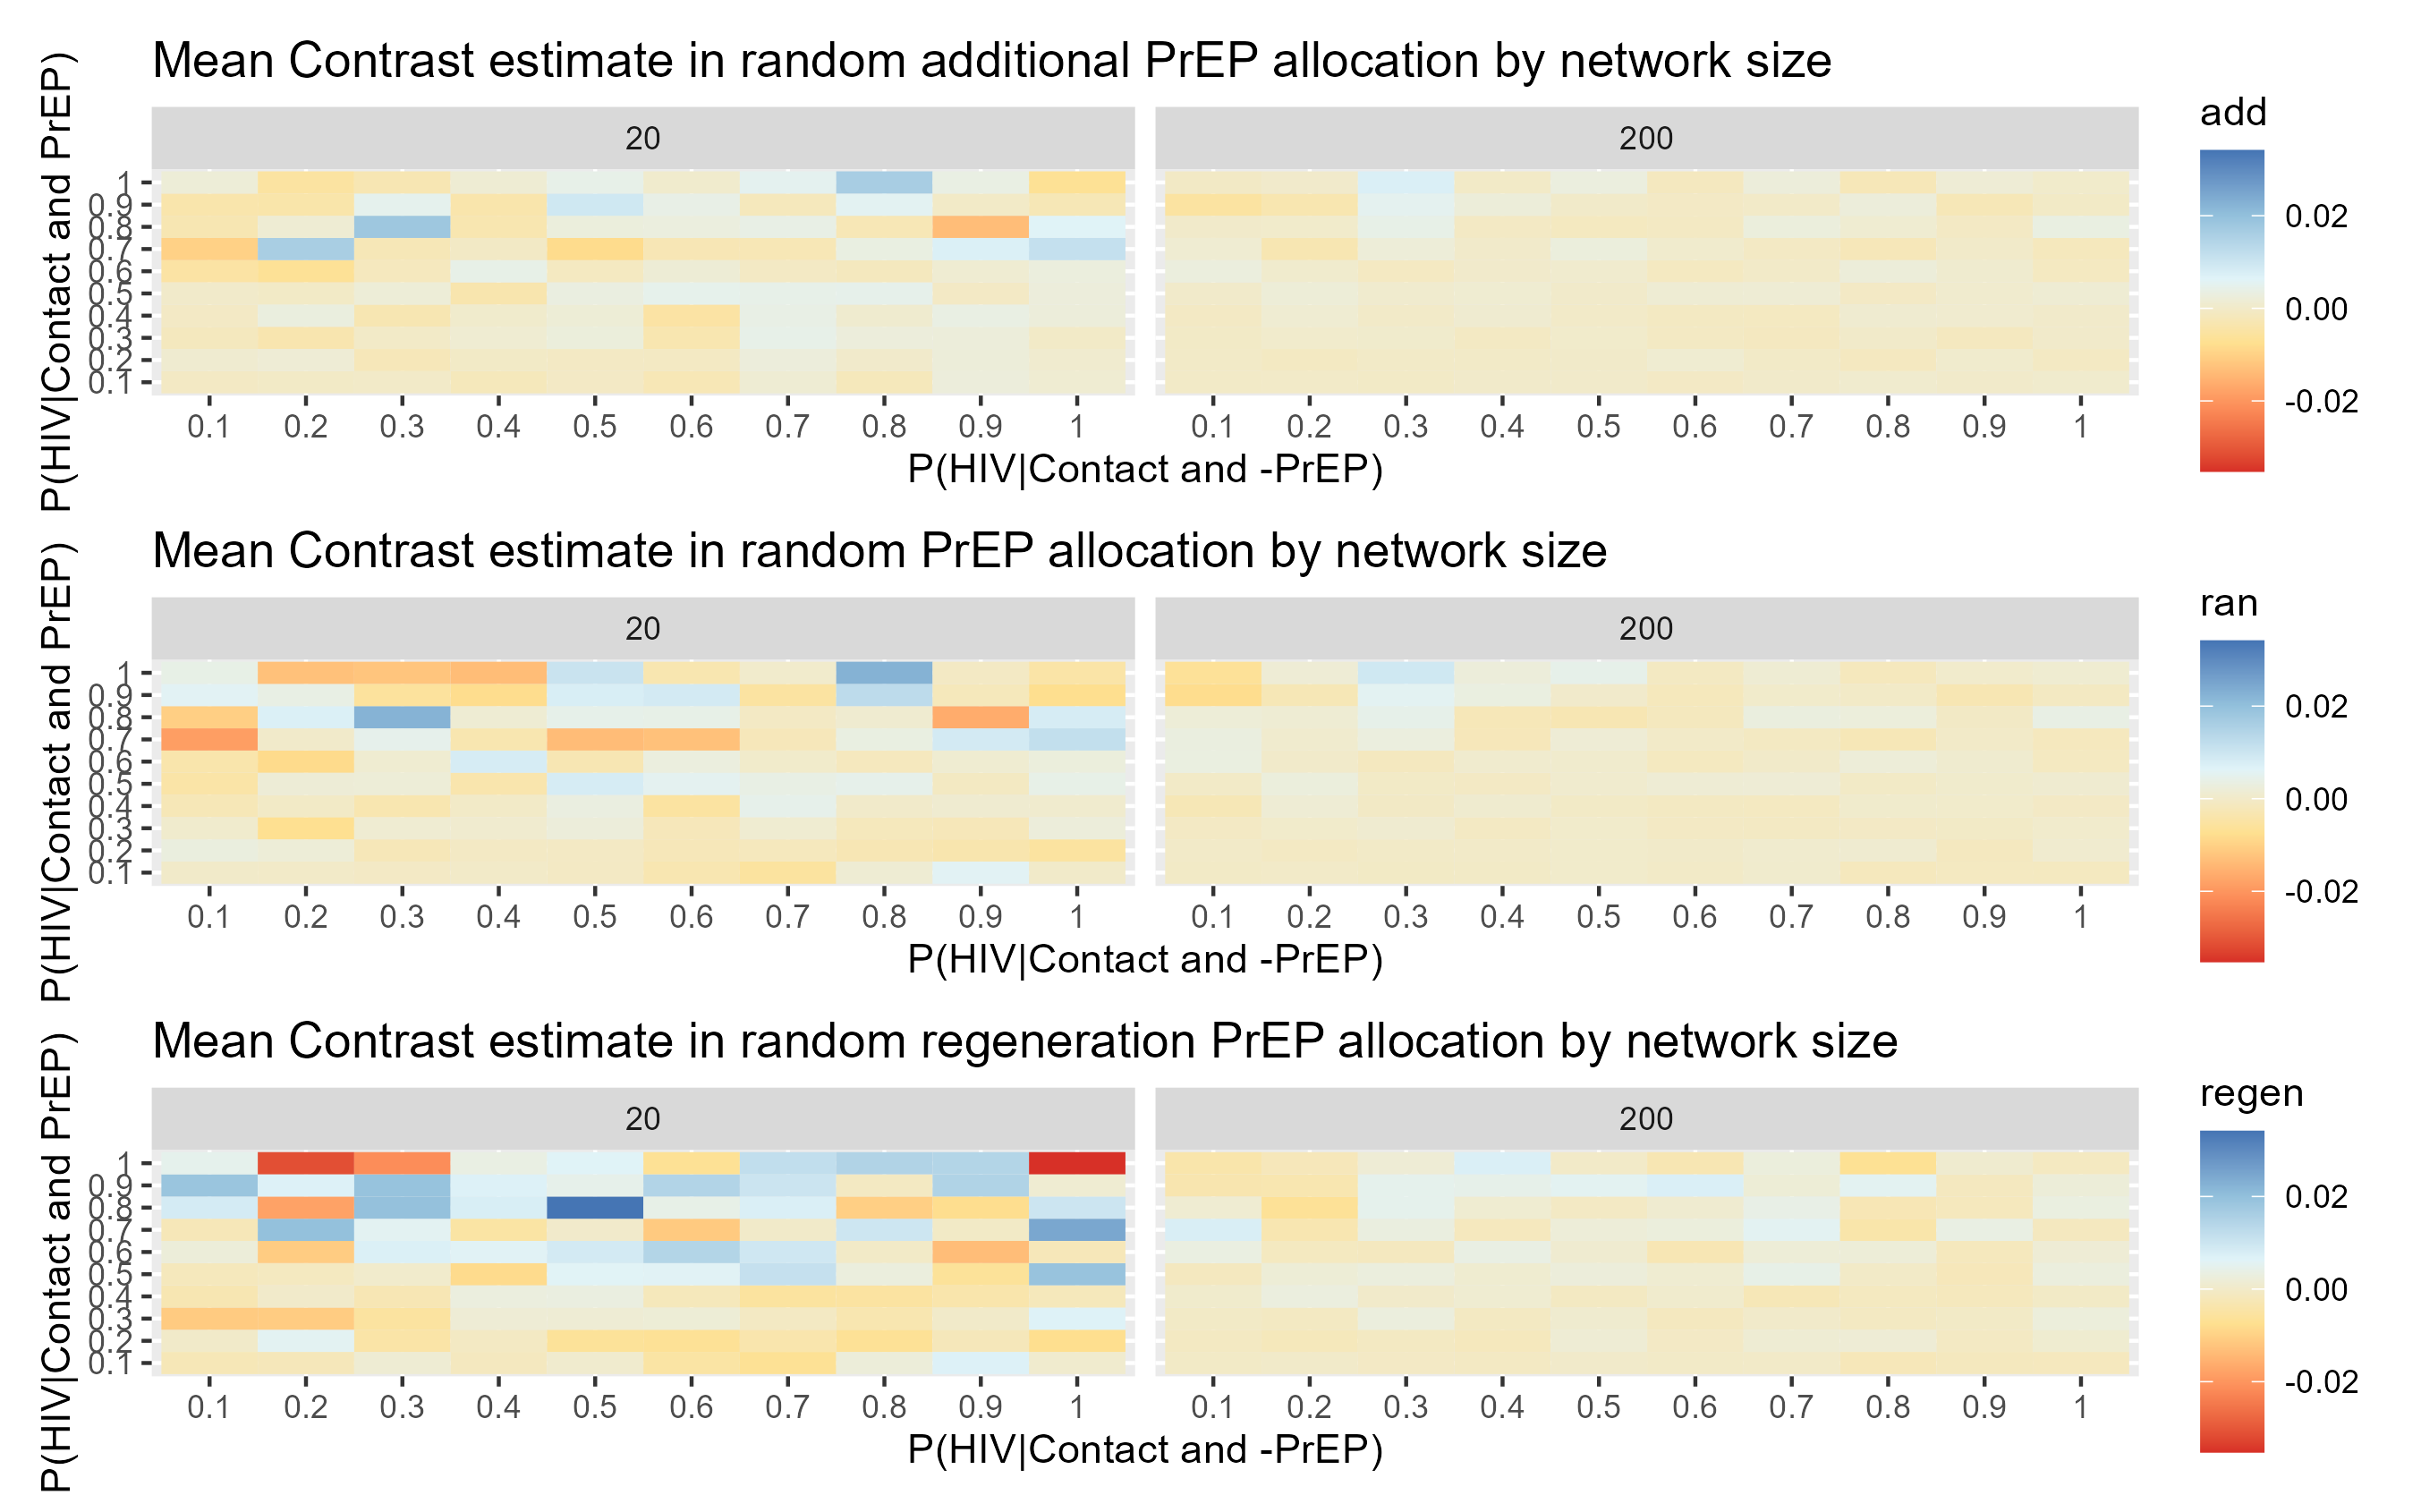
\includegraphics[scale=0.8]{Figures/Network Size Mean Plot.png}
    \caption{Mean Causal Contrast estimates stratified by Network Size/Graph Order. From top to bottom: "additive" Mean Contrast of random 20\% additional vs. random 20\% PrEP allocation control, ``random" Mean Contrast of random 40\% PrEP allocation vs. random 20\% control, ``regenerated" Mean Contrast of random 40\% allocation on regenerated network vs. random 20\% control. }
    \label{fig:Figure 7}
\end{figure}
\begin{figure}[H]
    \centering
    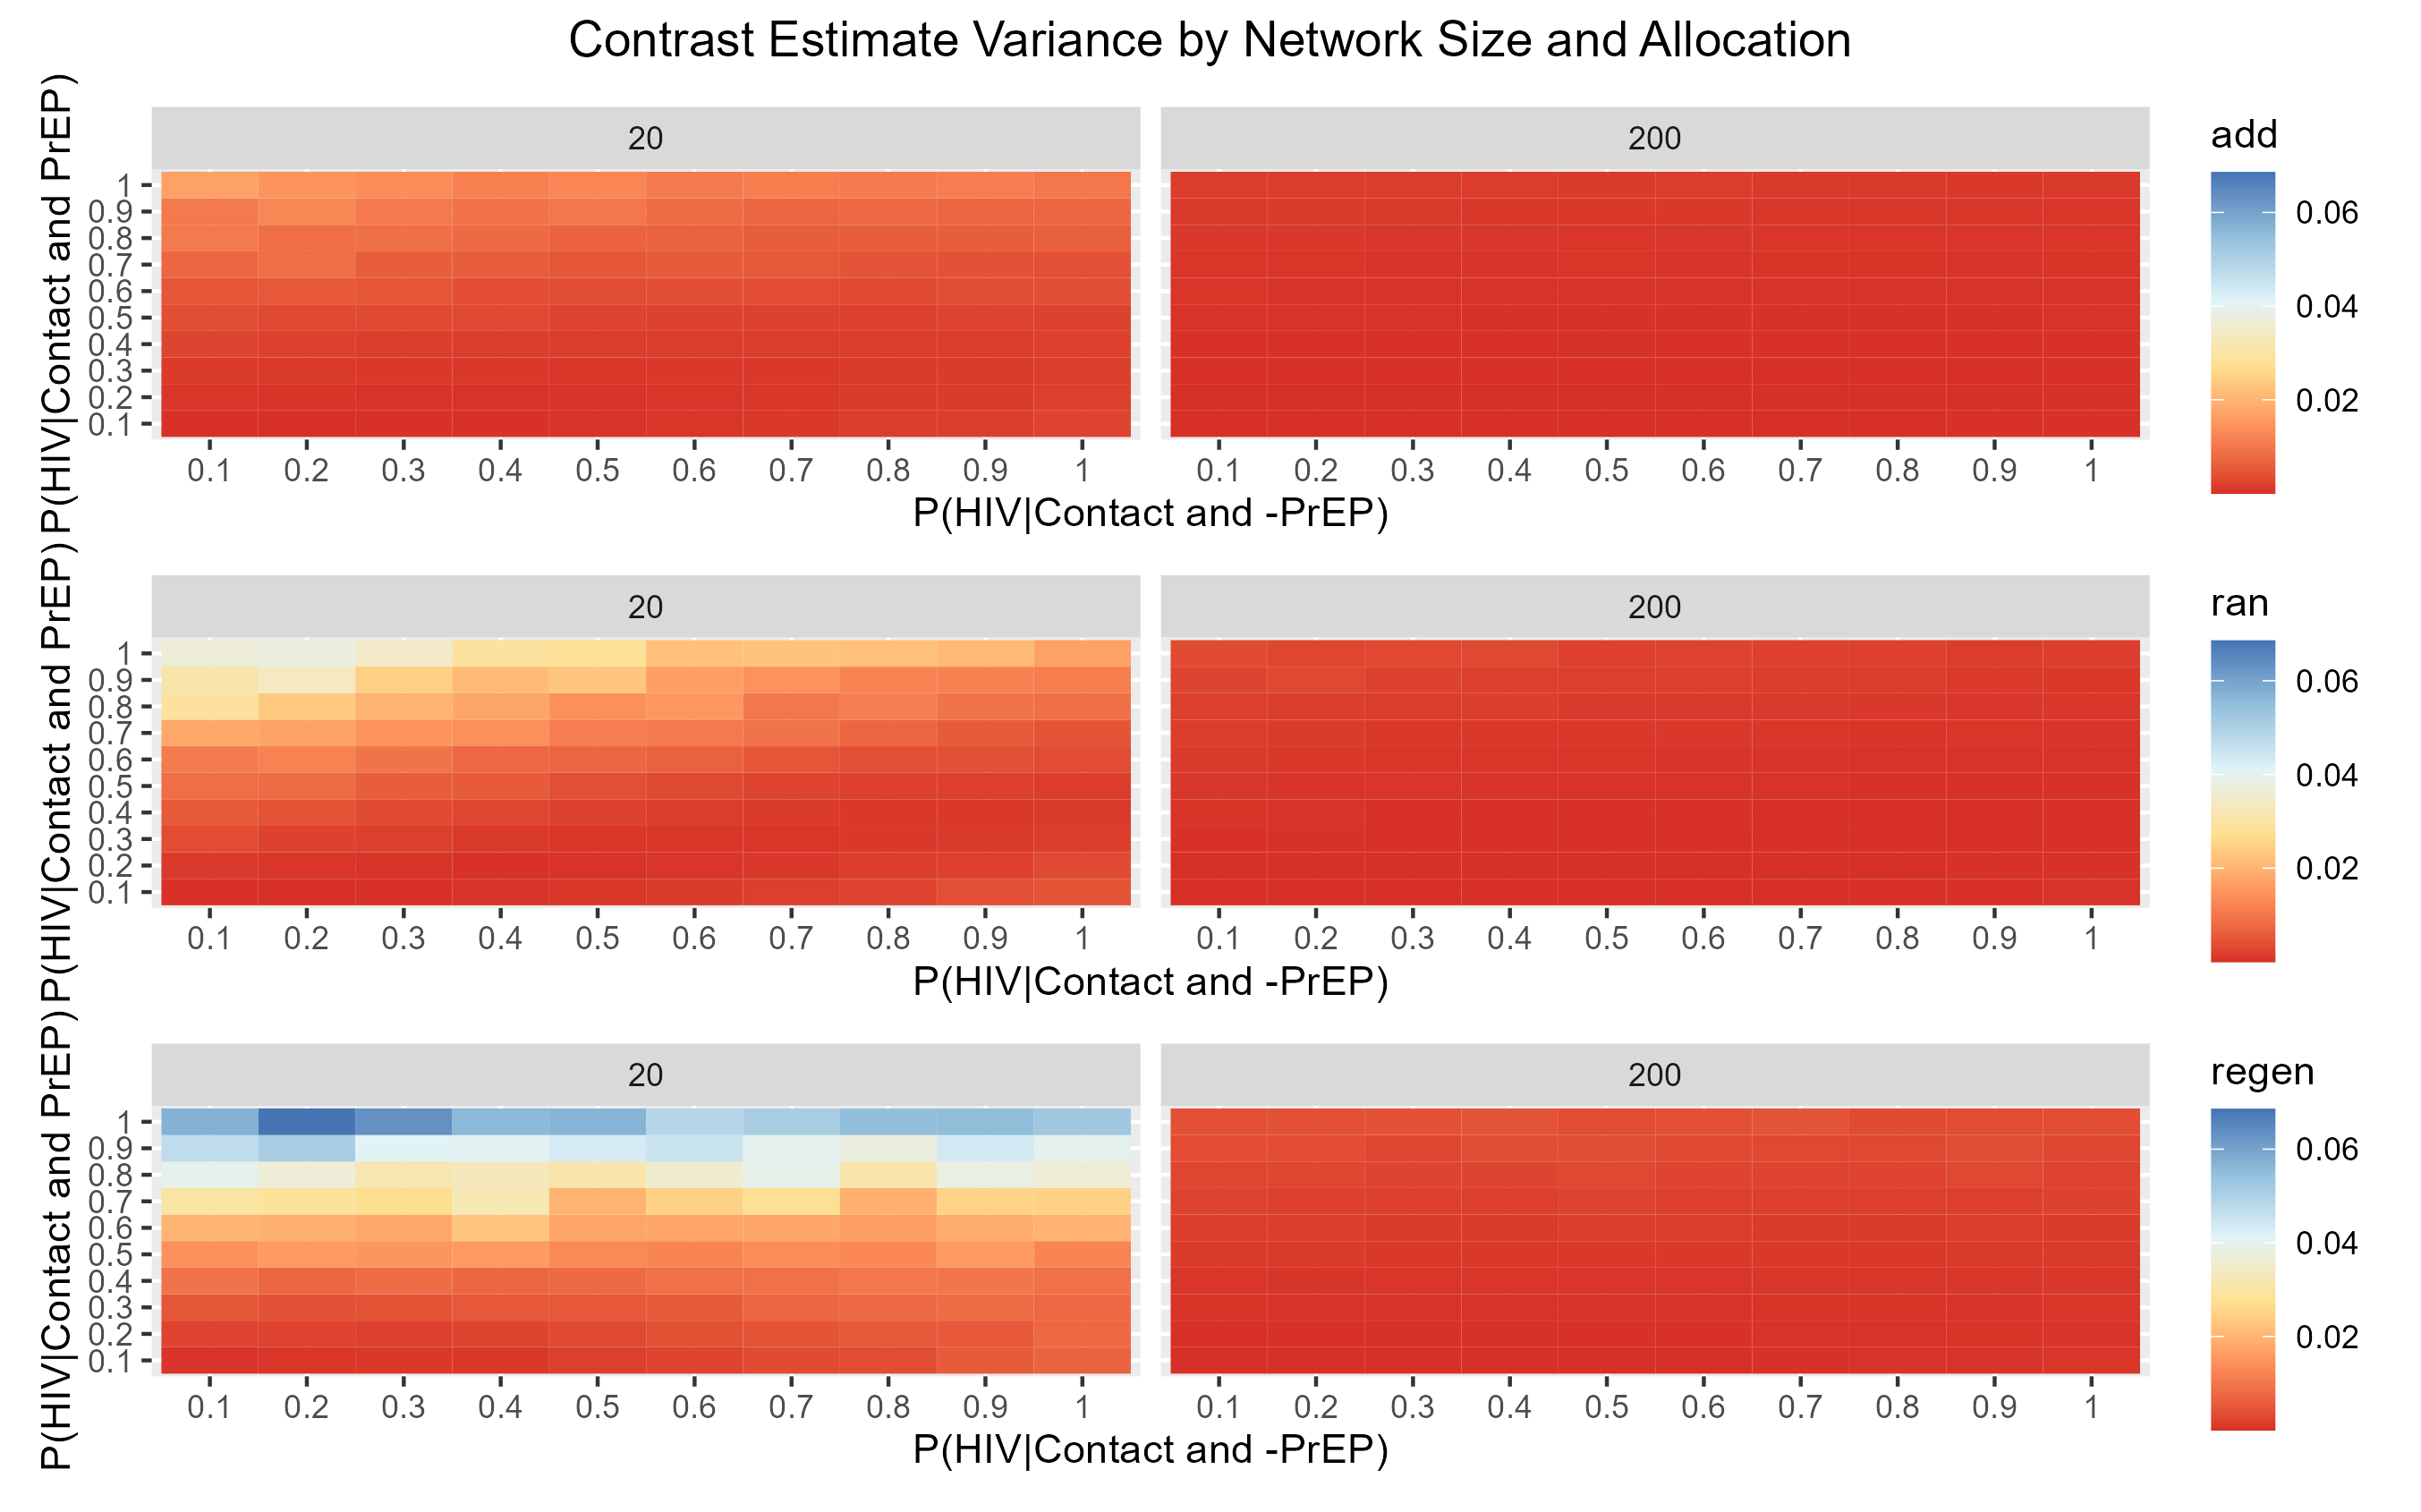
\includegraphics[scale=0.8]{Figures/Network Size Variance plots.png}
    \caption{Variance of Causal Contrast estimates stratified by Network Size/Graph Order. From top to bottom: ``additive" Variance of Contrast of random 20\% additional vs. random 20\% PrEP allocation control, ``random" Variance of Contrast of random 40\% PrEP allocation vs. random 20\% control, ``regenerated" Variance of Contrast of random 40\% allocation on regenerated network vs. random 20\% control.}
    \label{fig:Figure 8}
\end{figure}
\subsubsection{Effect Modification by Sample Size}
\begin{figure}[H]
    \centering
    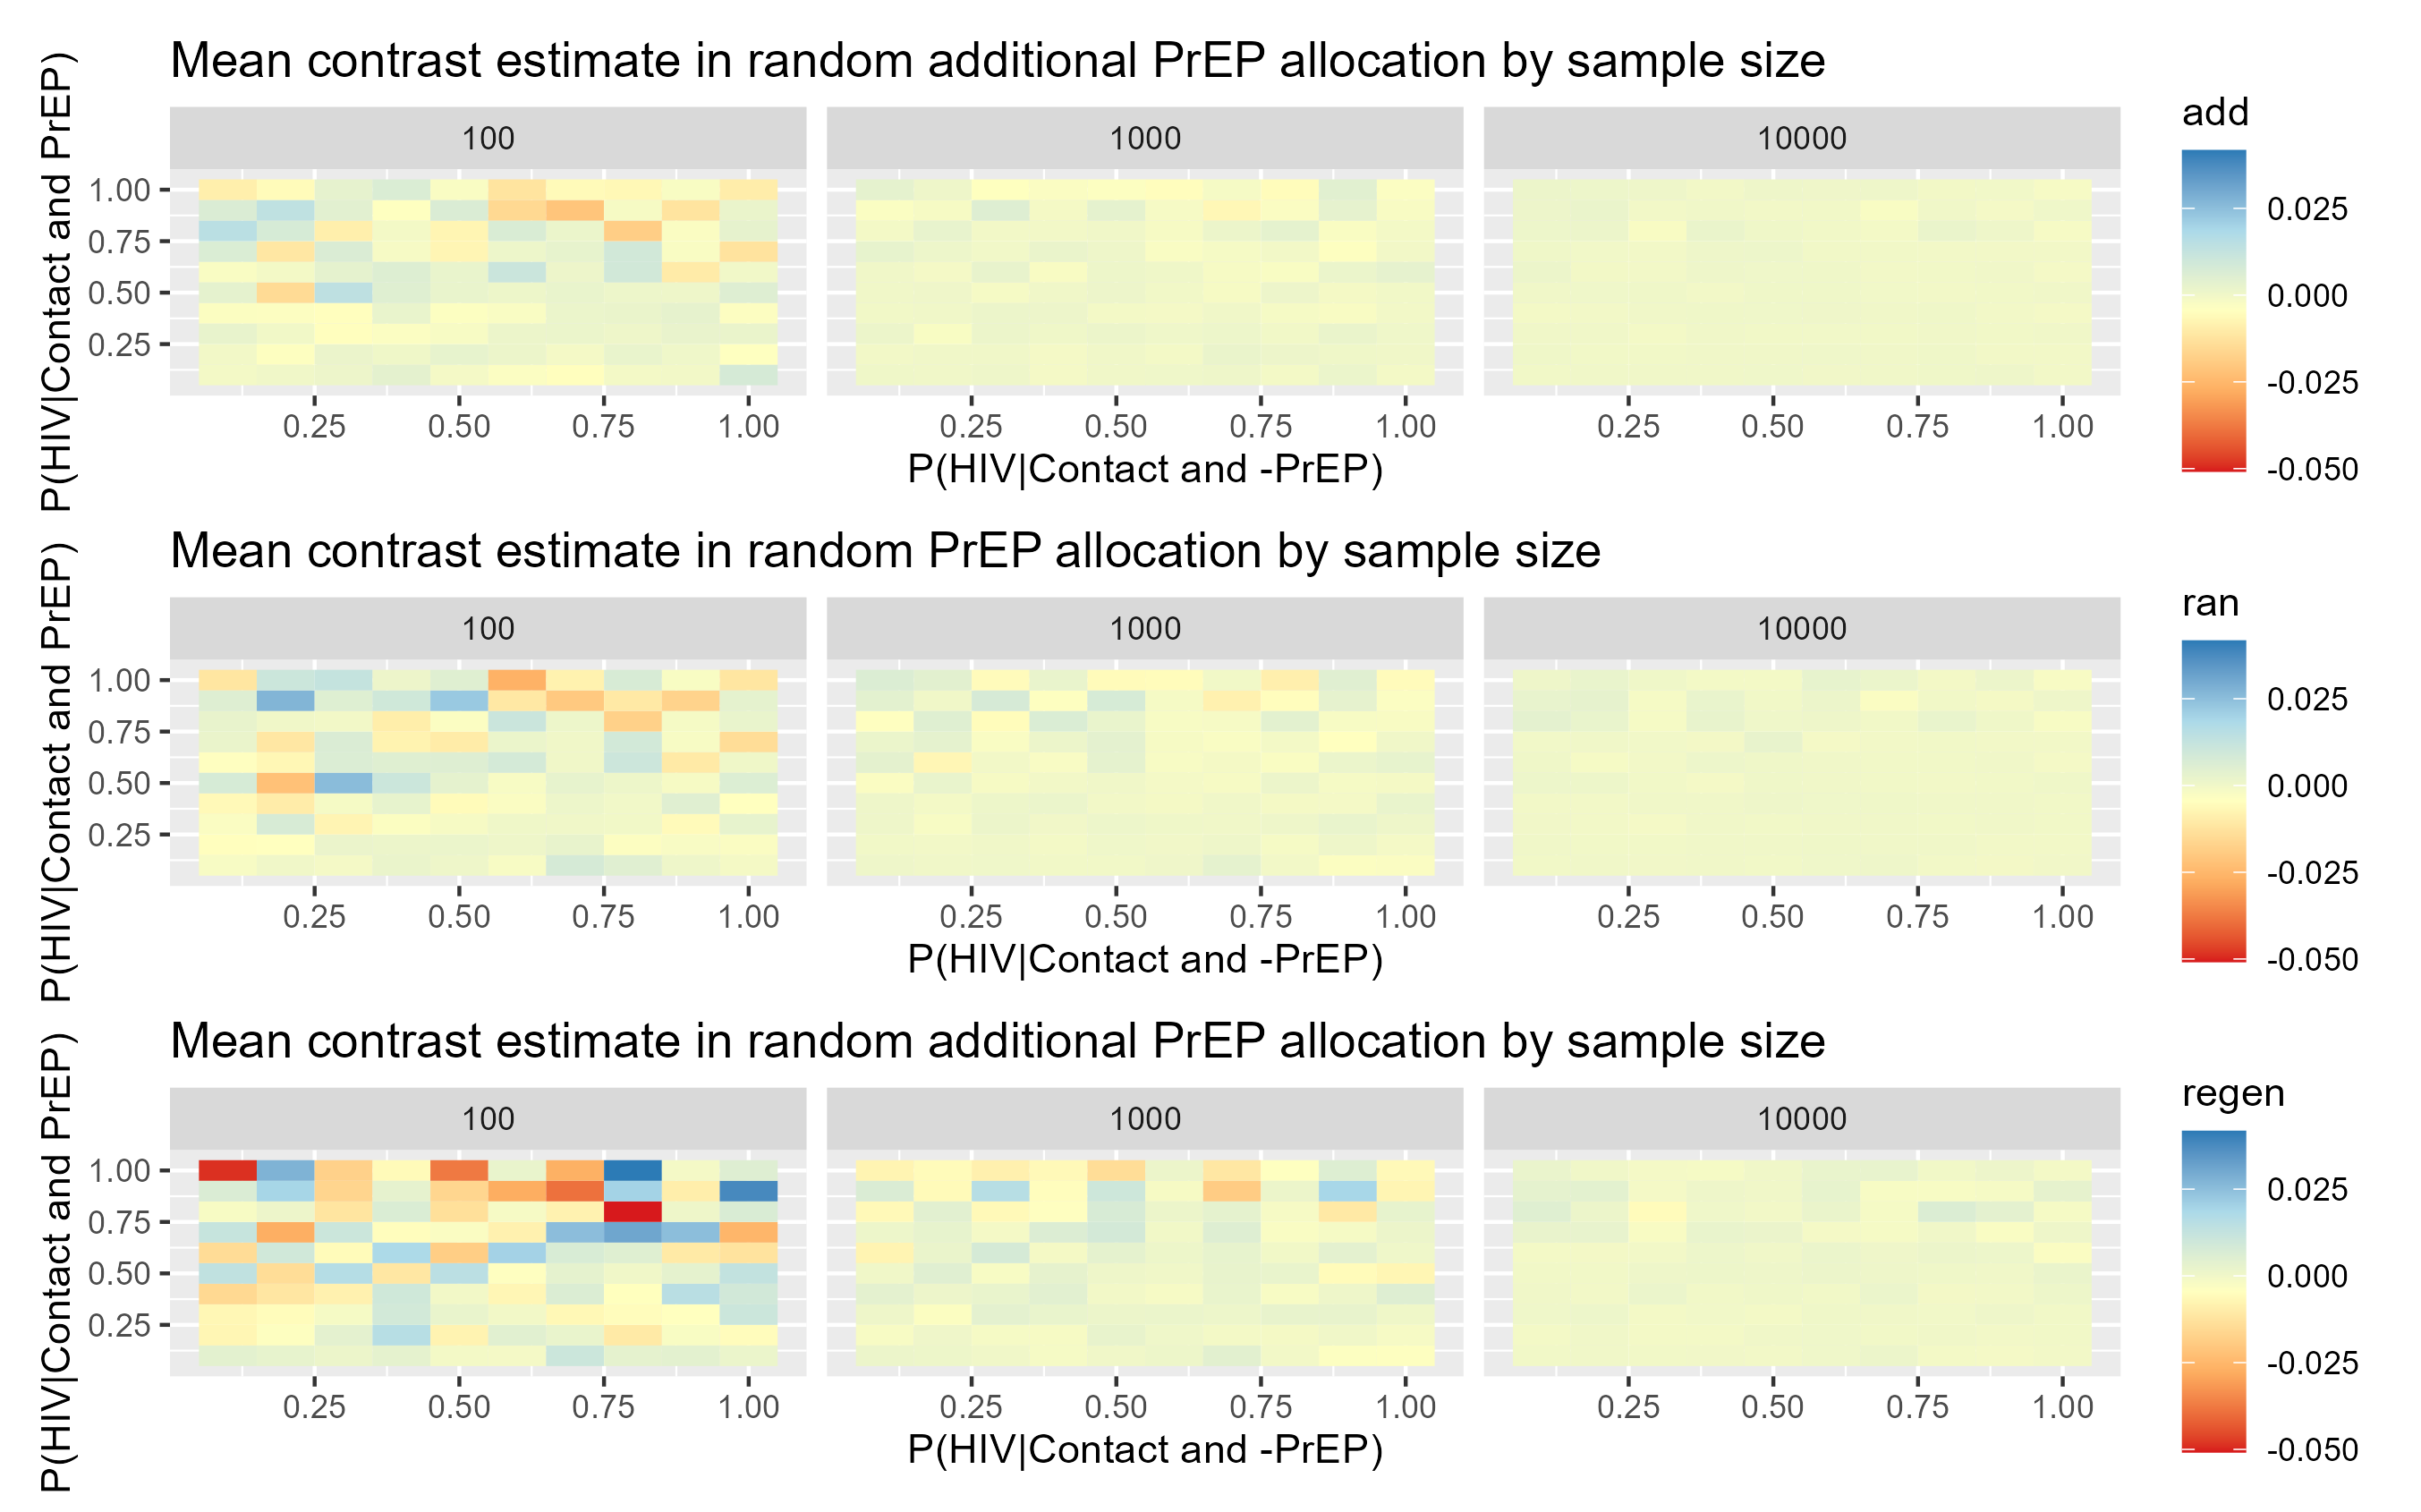
\includegraphics[scale=0.8]{Figures/Sample size Mean plots.png}
    \caption{Mean Causal Contrast estimates stratified by resampling sample size. From top to bottom: ``additive" Mean Contrast of random 20\% additional vs. random 20\% PrEP allocation control, ``random" Mean Contrast of random 40\% PrEP allocation vs. random 20\% control, ``regenerated" Mean Contrast of random 40\% allocation on regenerated network vs. random 20\% control.}
    \label{fig:Figure 9}
\end{figure}
\begin{figure}[H]
    \centering
    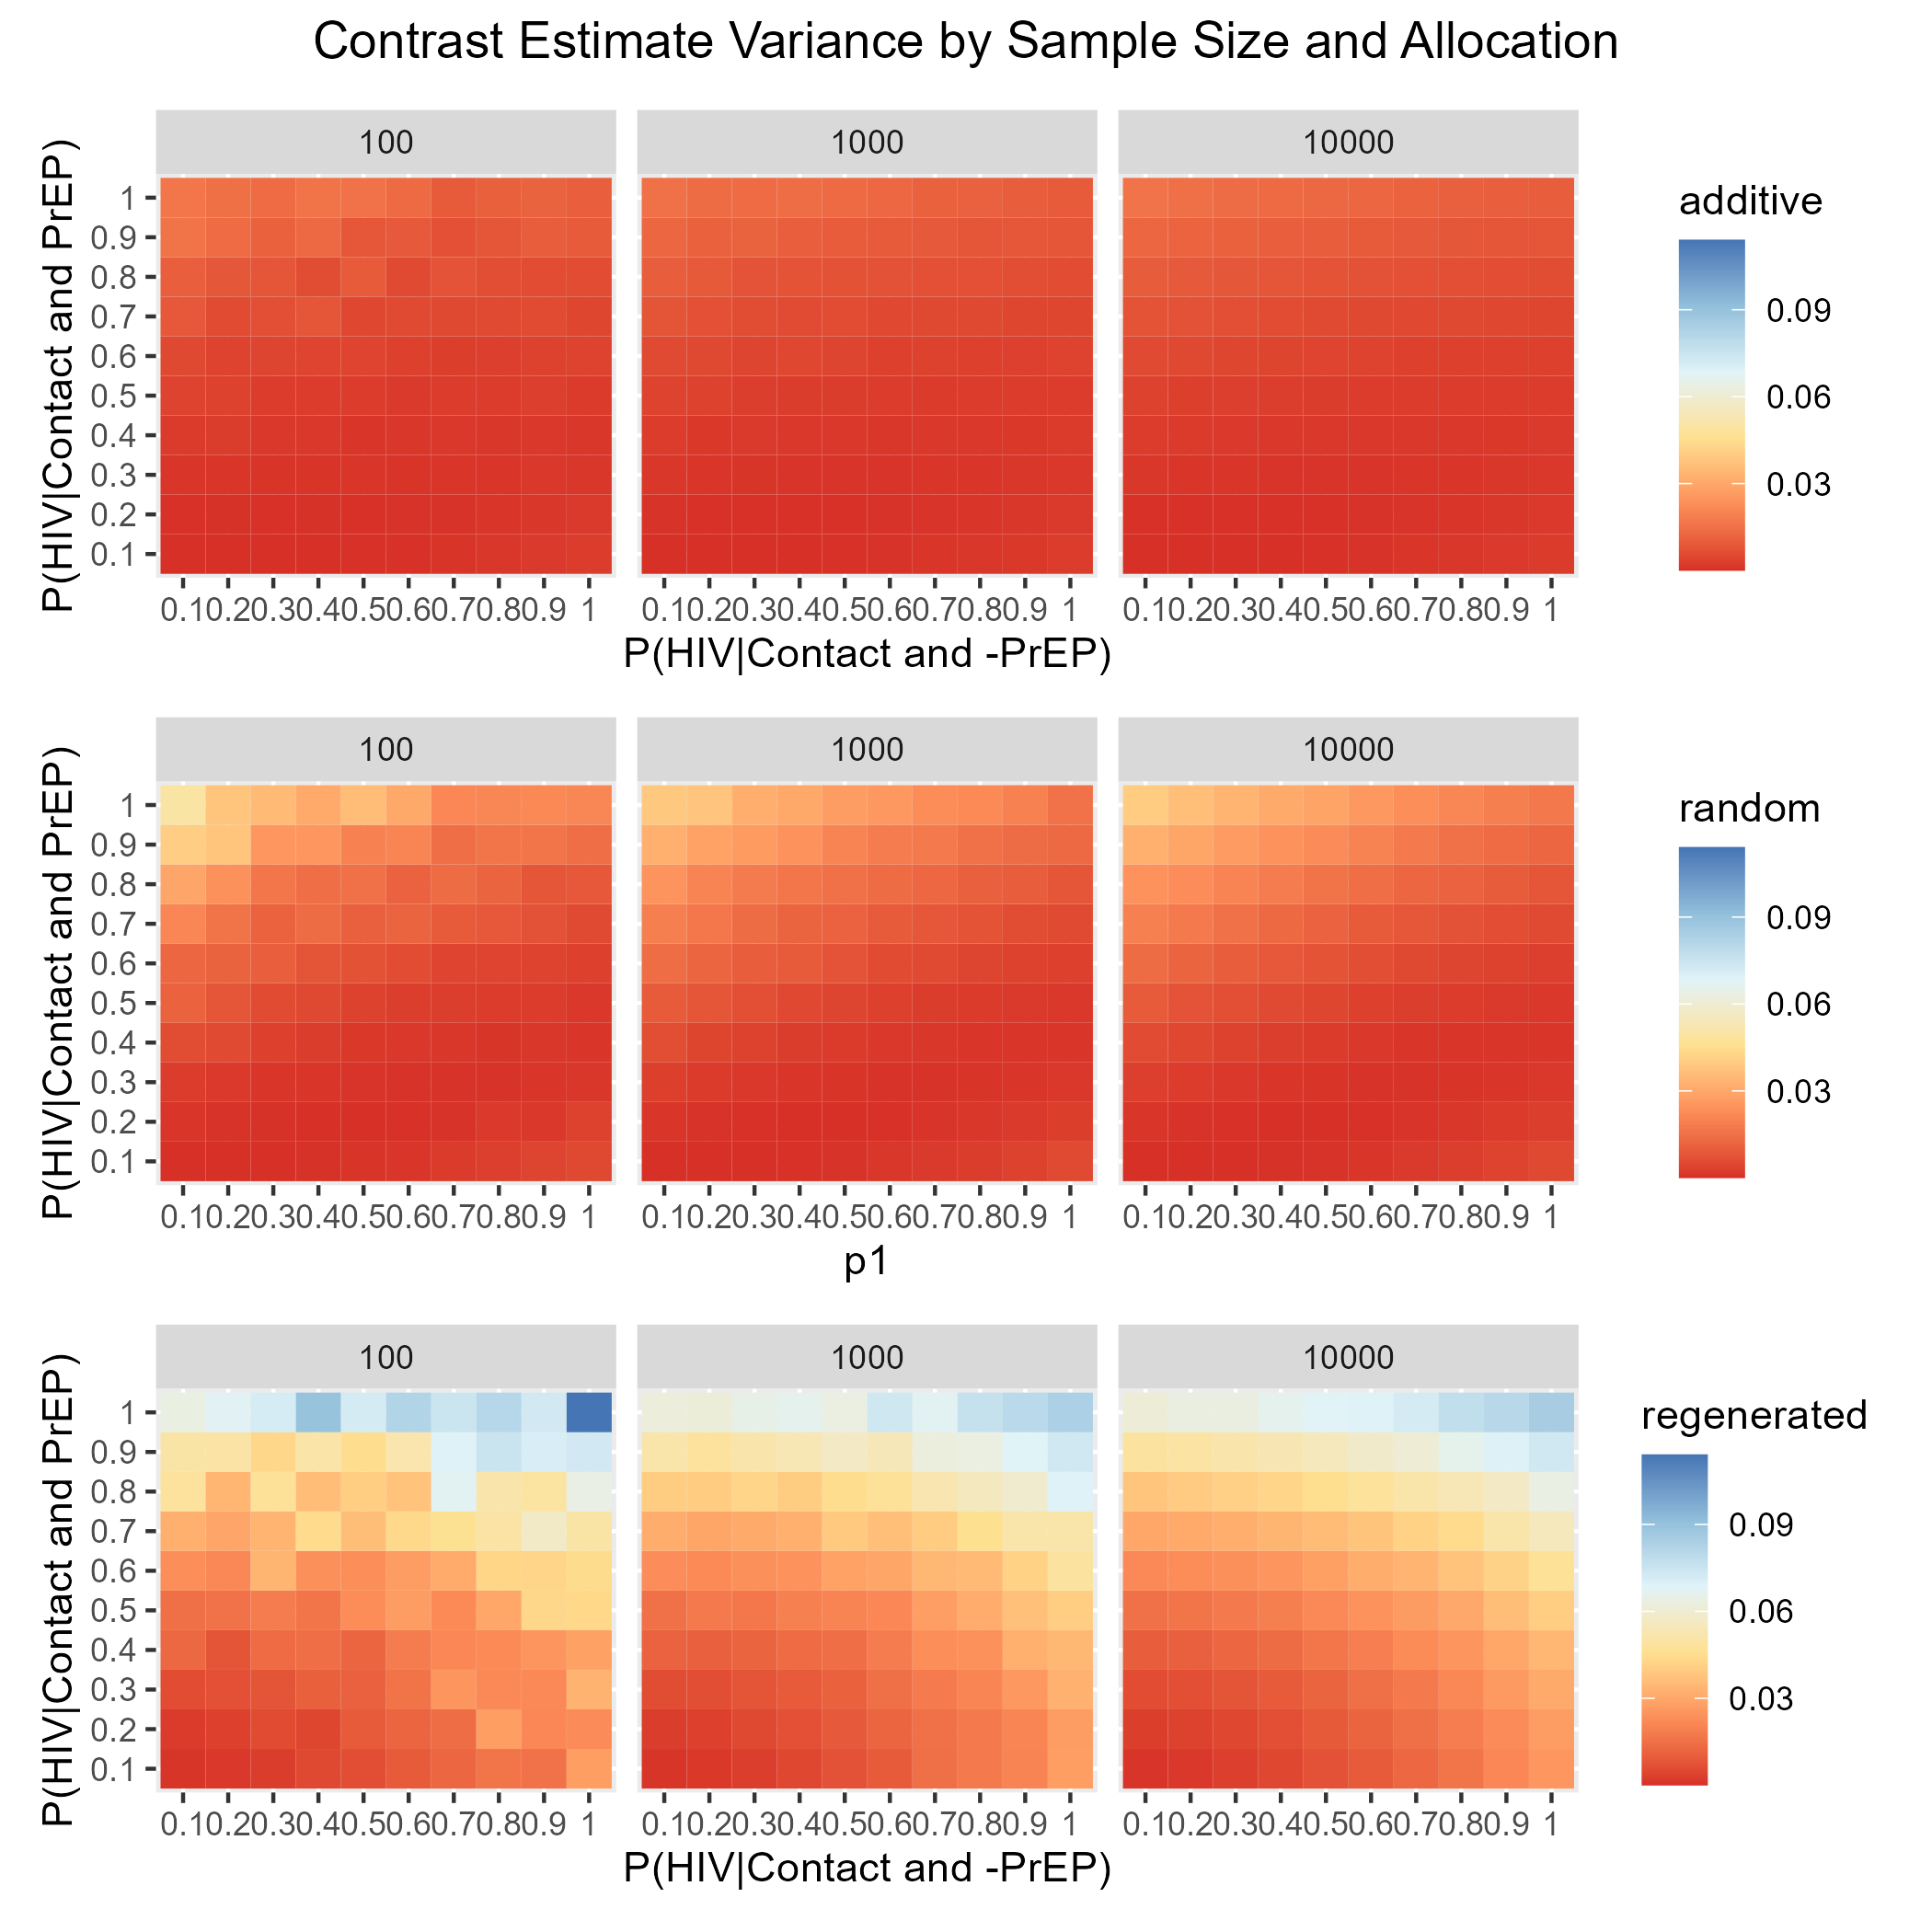
\includegraphics[scale=0.8]{Figures/Sample Size Variance plots.png}
    \caption{Variance of Causal Contrast estimates stratified by resampling sample size. From top to bottom: ``additive" Variance of Contrast of random 20\% additional vs. random 20\% PrEP allocation control, ``random" Variance of Contrast of random 40\% PrEP allocation vs. random 20\% control, ``regenerated" Variance of Contrast of random 40\% allocation on regenerated network vs. random 20\% control.}
    \label{fig:Figure 10}
\end{figure}
\subsubsection{Effect Modification by HIV Prevalence}
\begin{figure}[H]
    \centering
    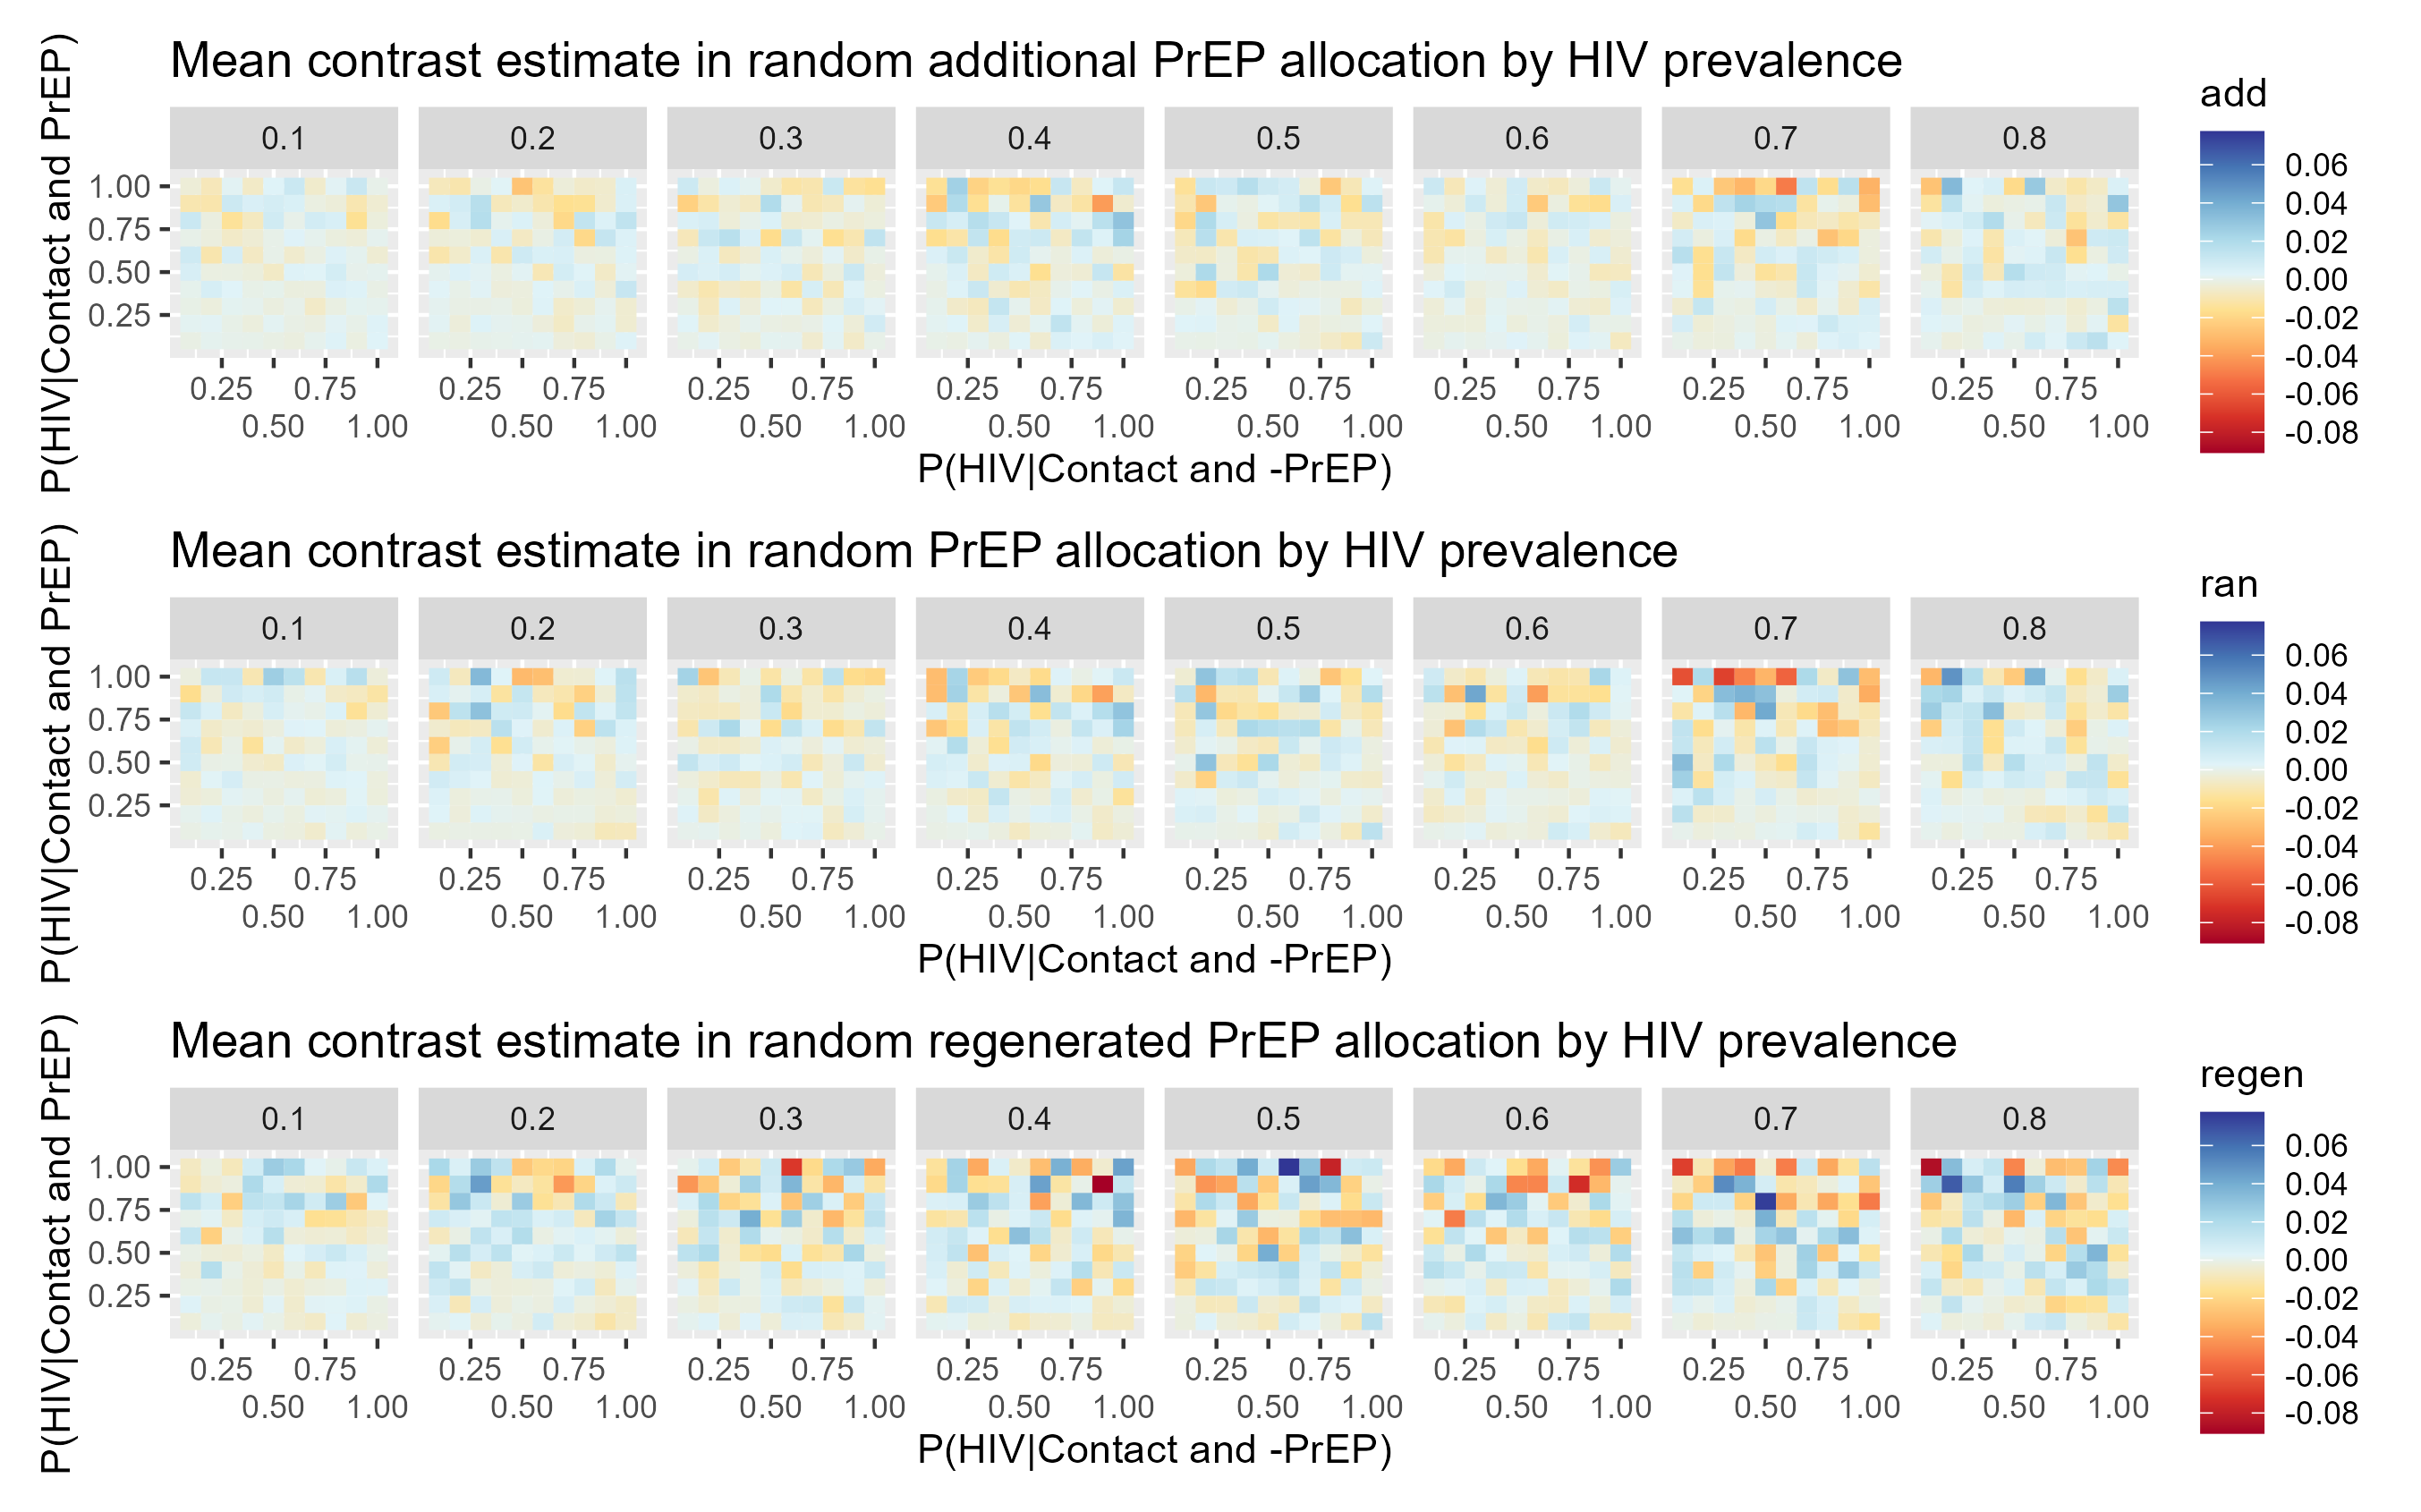
\includegraphics[scale=0.8]{Figures/HIV Prevalence Mean plots.png}
    \caption{Mean Causal Contrast estimates stratified by HIV Prevalence. From top to bottom: ``additive" Mean Contrast of random 20\% additional vs. random 20\% PrEP allocation control, ``random" Mean Contrast of random 40\% PrEP allocation vs. random 20\% control, ``regenerated" Mean Contrast of random 40\% allocation on regenerated network vs. random 20\% control.}
    \label{fig:Figure 11}
\end{figure}
\begin{figure}[H]
    \centering
    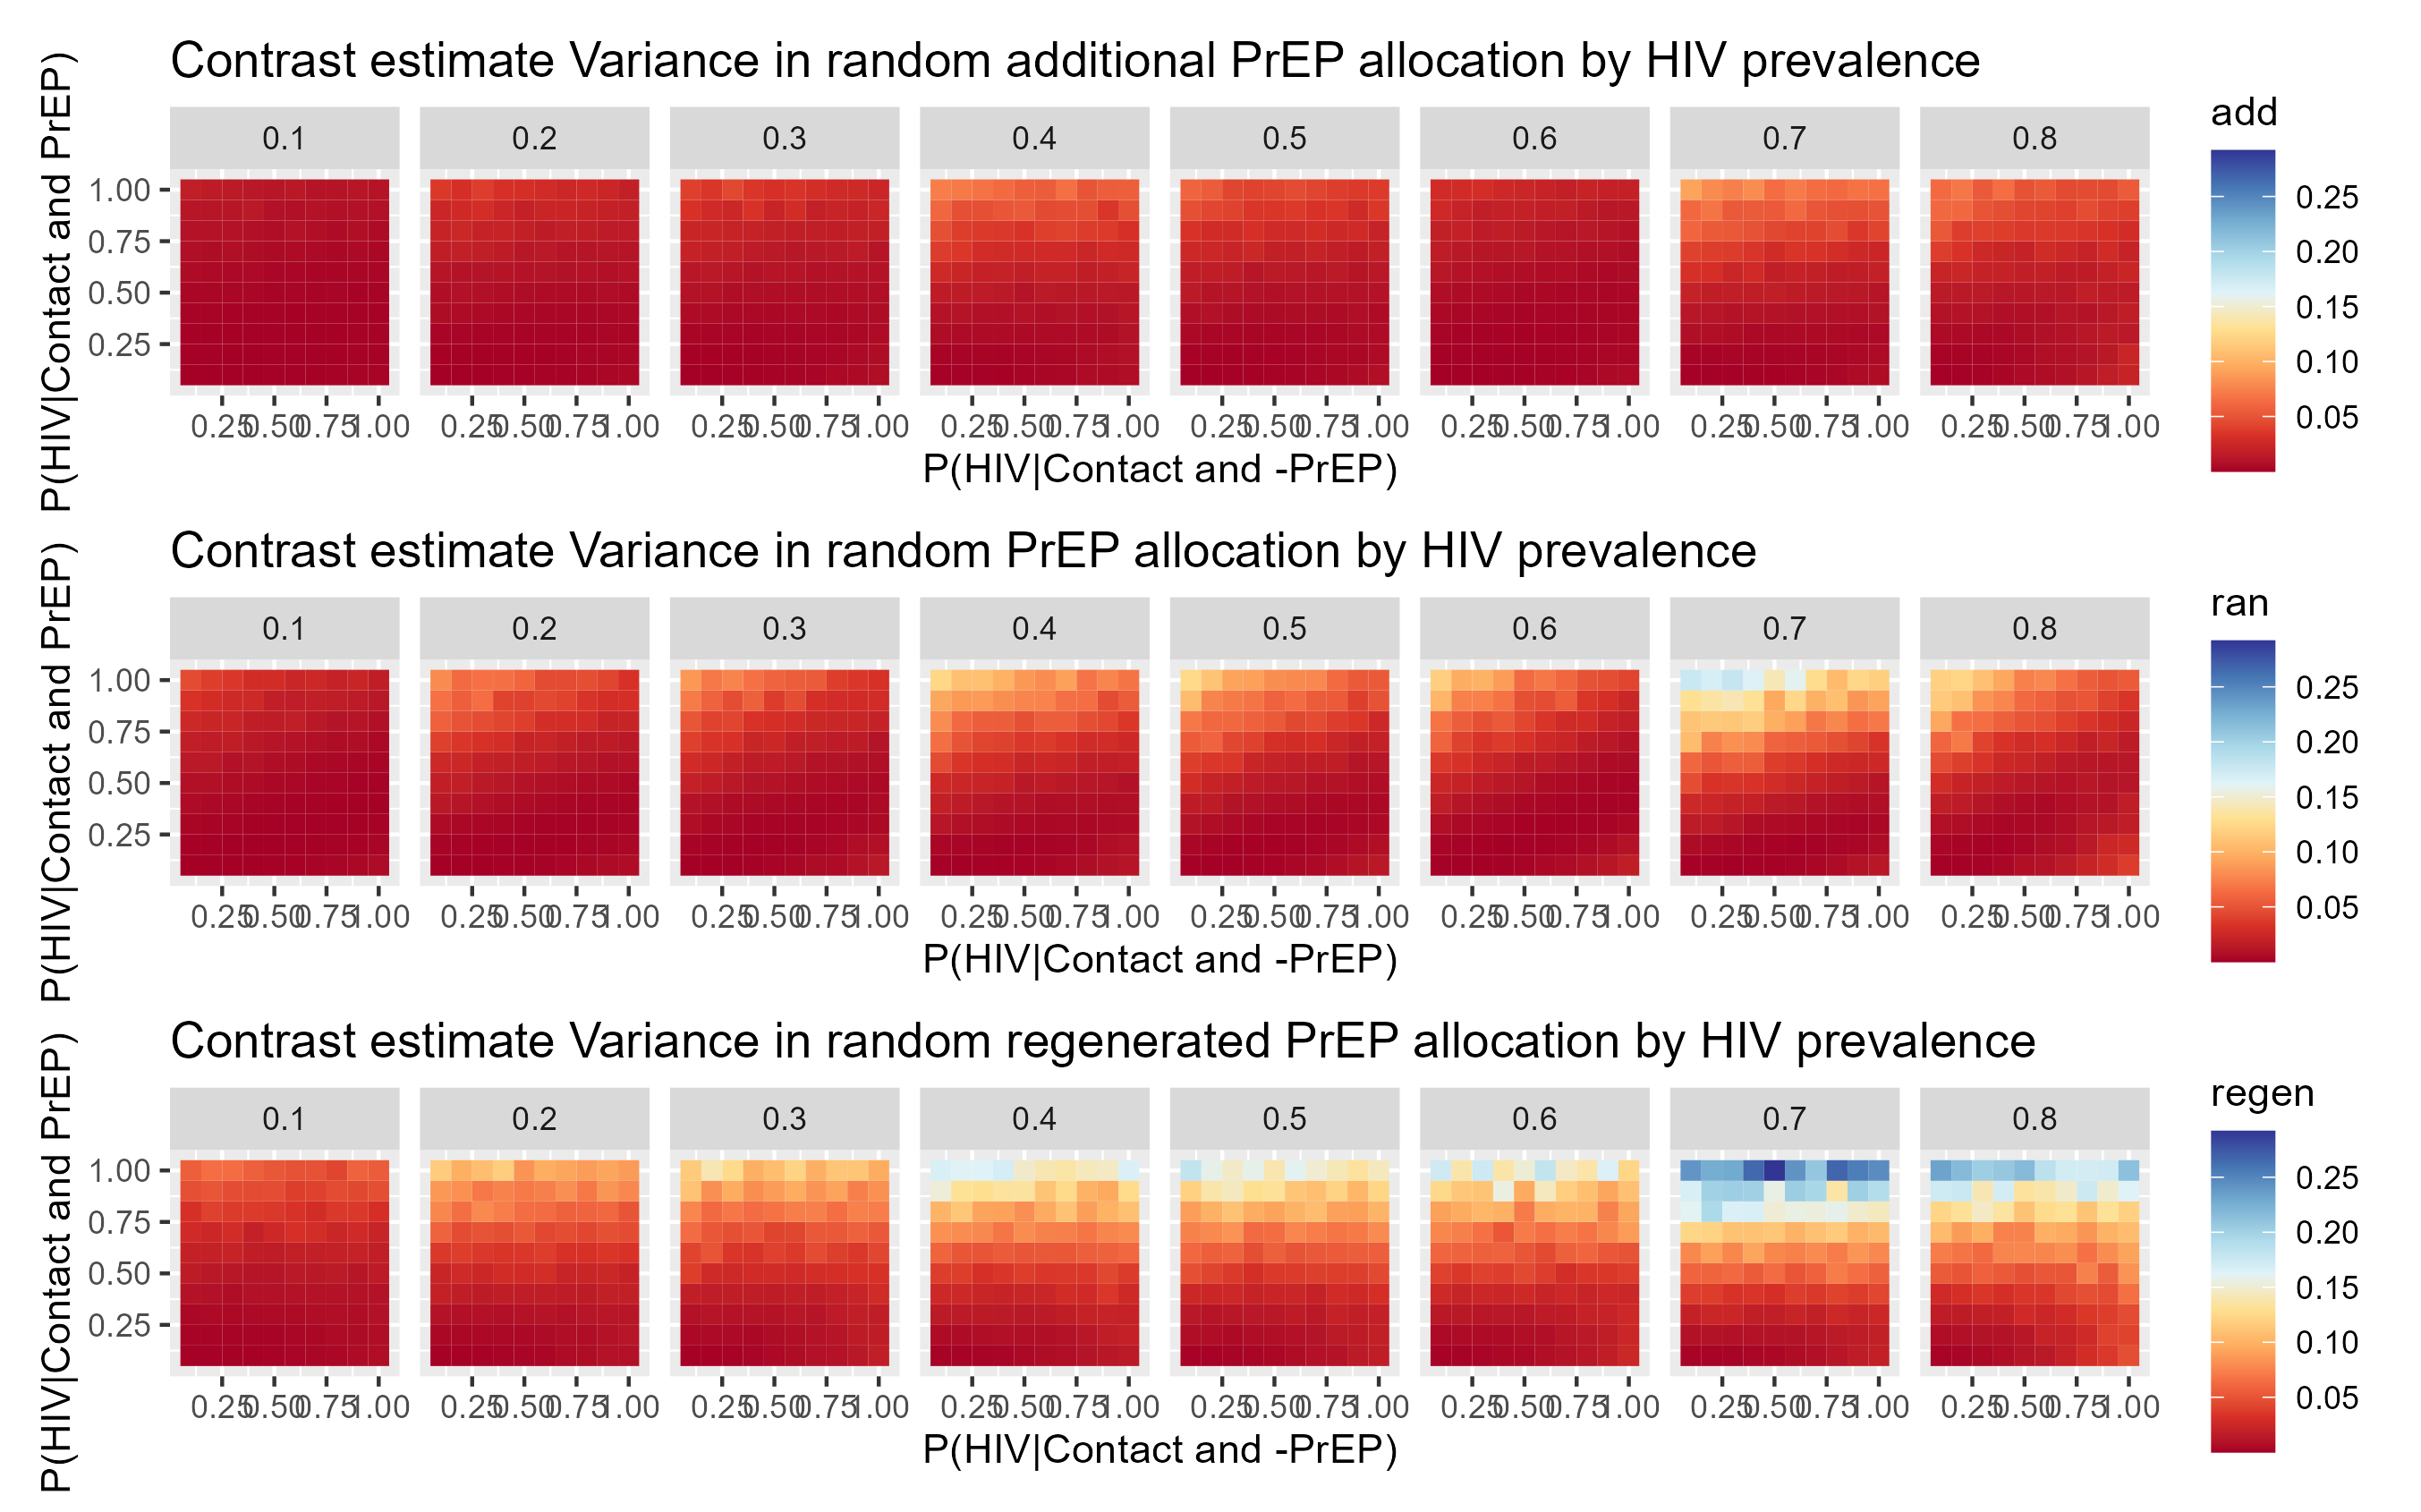
\includegraphics[scale=0.35]{Figures/HIV Prevalence Variance plots.png}
    \caption{Variance of Causal Contrast estimates stratified by HIV Prevalence. From top to bottom: ``additive" Variance of Contrast of random 20\% additional vs. random 20\% PrEP allocation control, ``random" Variance of Contrast of random 40\% PrEP allocation vs. random 20\% control, ``regenerated" Variance of Contrast of random 40\% allocation on regenerated network vs. random 20\% control.}
    \label{fig:Figure 12}
\end{figure}
\subsubsection{Effect Modification by $\mathbb{P}\left[\text{HIV } \vert \text{ PrEP}^{c}\right]$}
\begin{figure}[H]
    \centering
    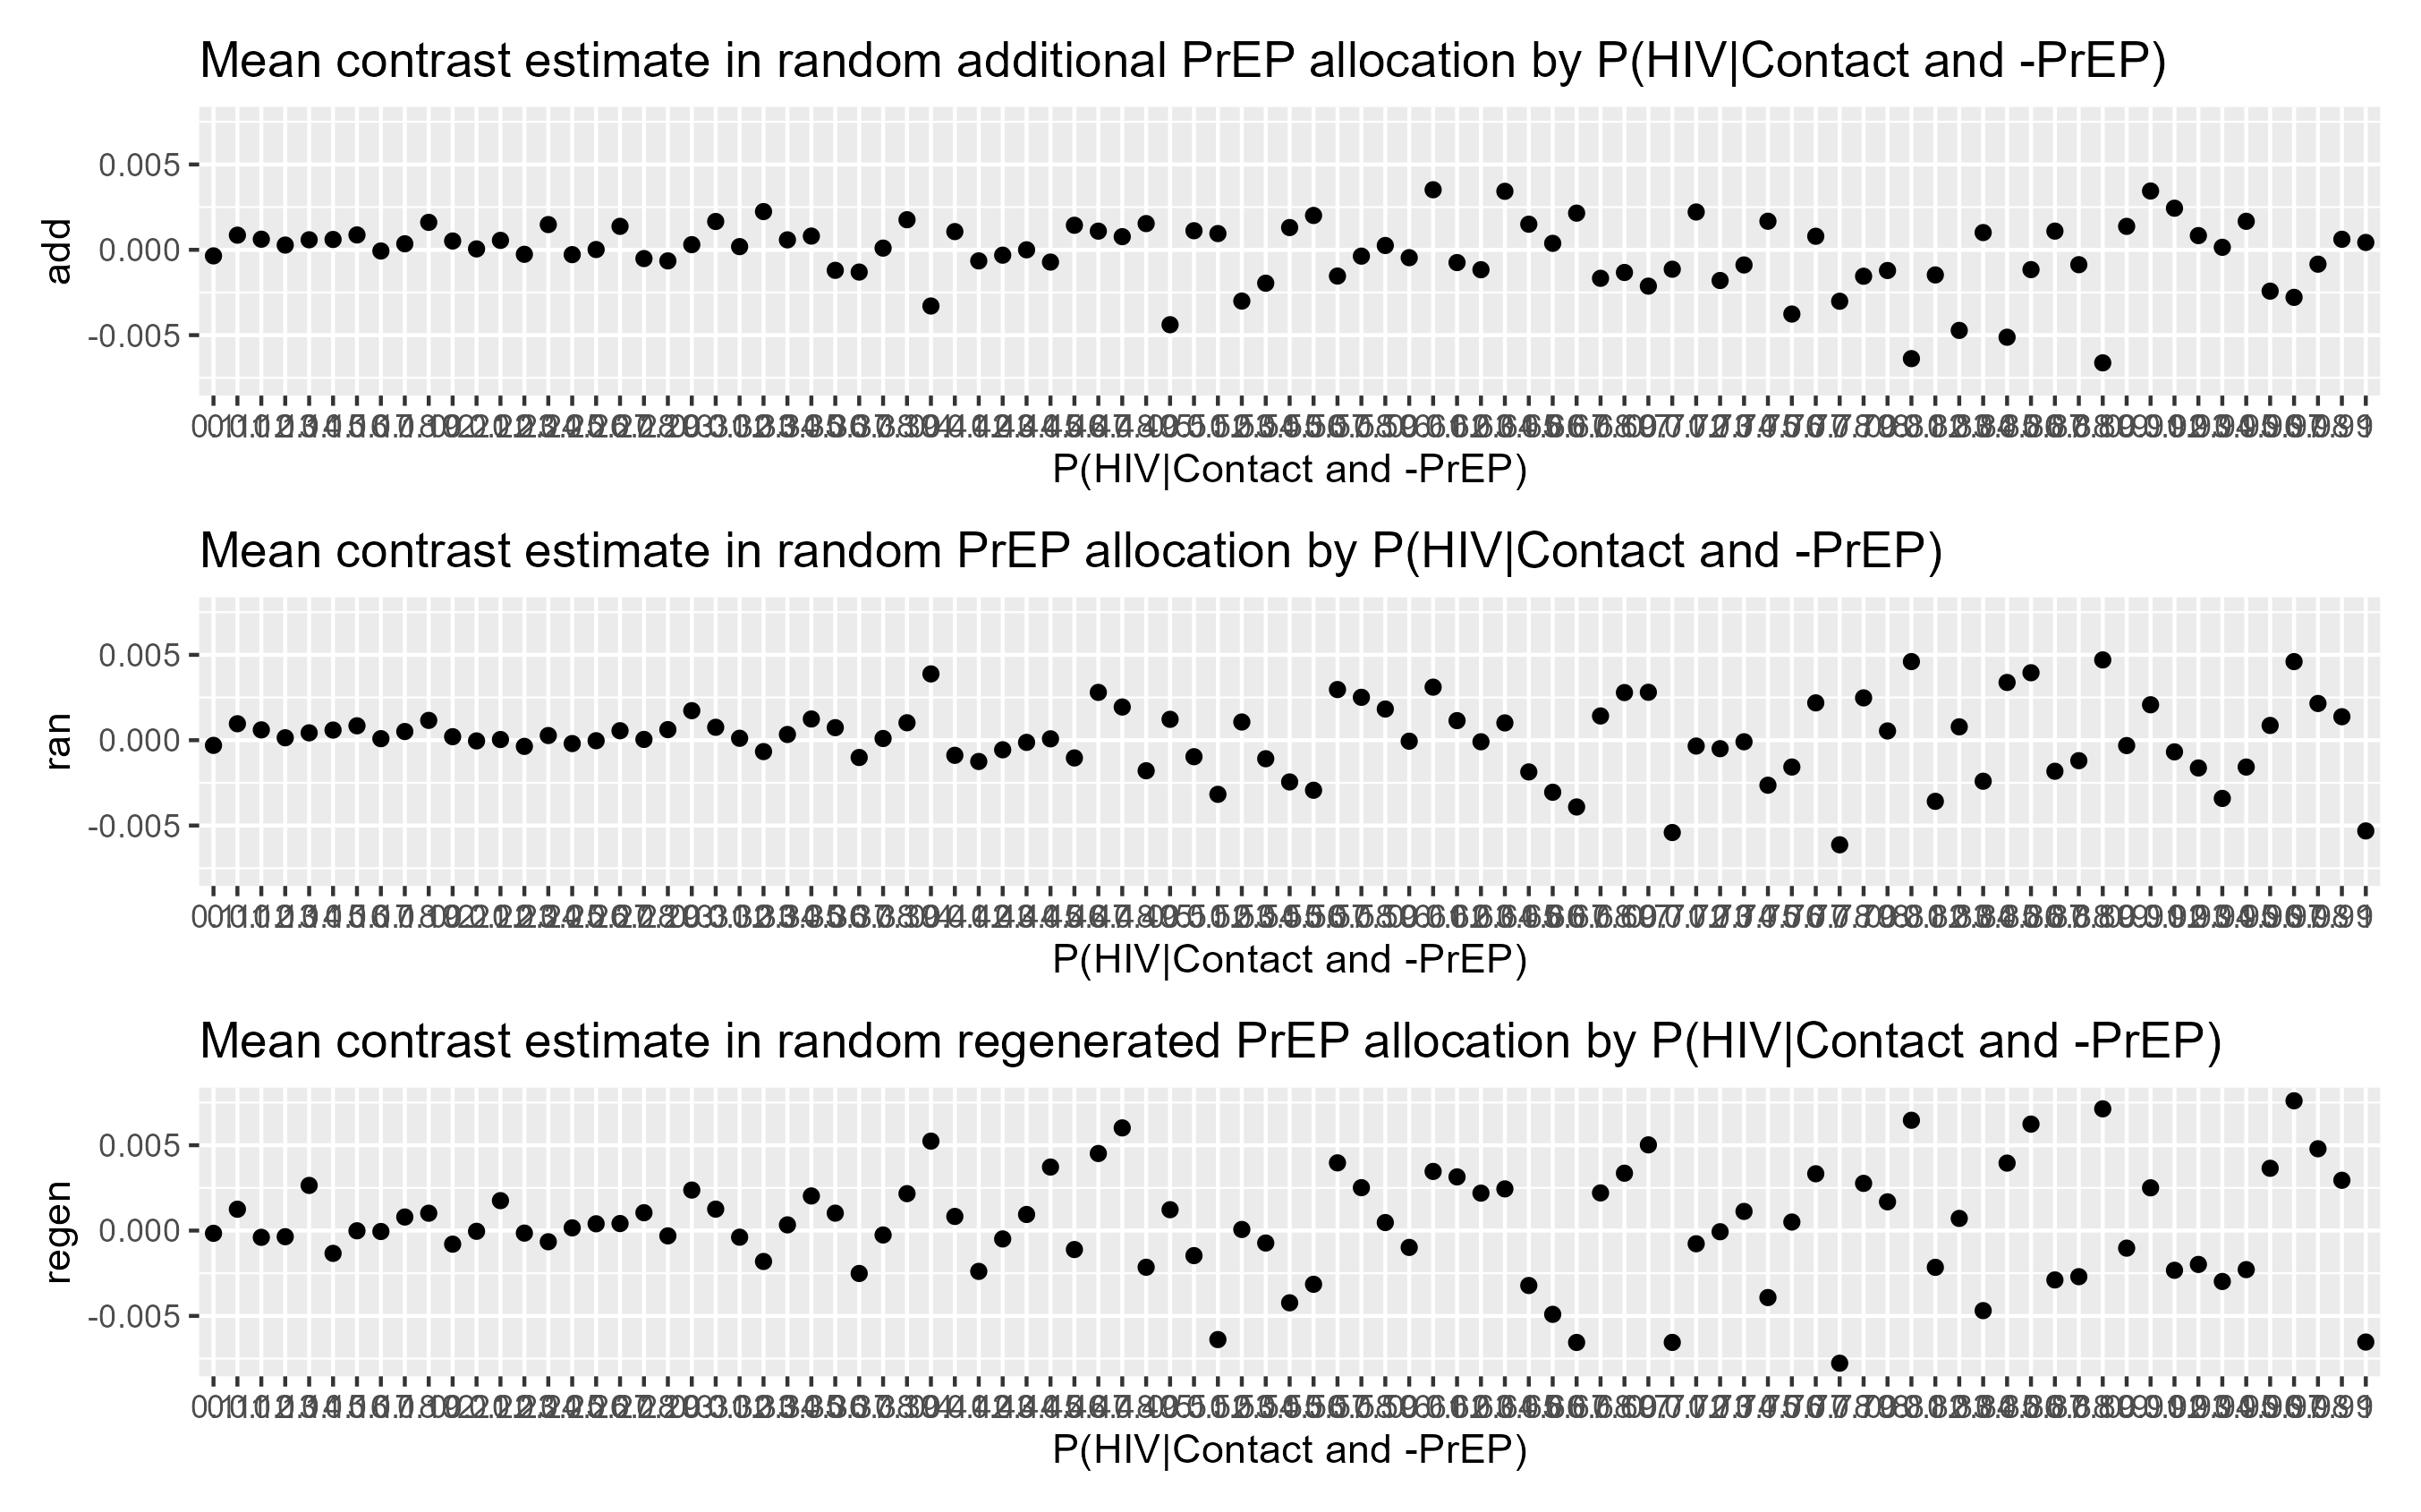
\includegraphics[scale=0.75]{Figures/p1 Mean plots.png}
    \caption{Mean Causal Contrast estimates as $\mathbb{P}\left[\text{HIV } \vert \text{ PrEP}^{c}\right]$ increases . From top to bottom: ``additive" Mean Contrast of random 20\% additional vs. random 20\% PrEP allocation control, ``random" Mean Contrast of random 40\% PrEP allocation vs. random 20\% control, ``regenerated" Mean Contrast of random 40\% allocation on regenerated network vs. random 20\% control.}
    \label{fig:Figure 13}
\end{figure}
\begin{figure}[H]
    \centering
    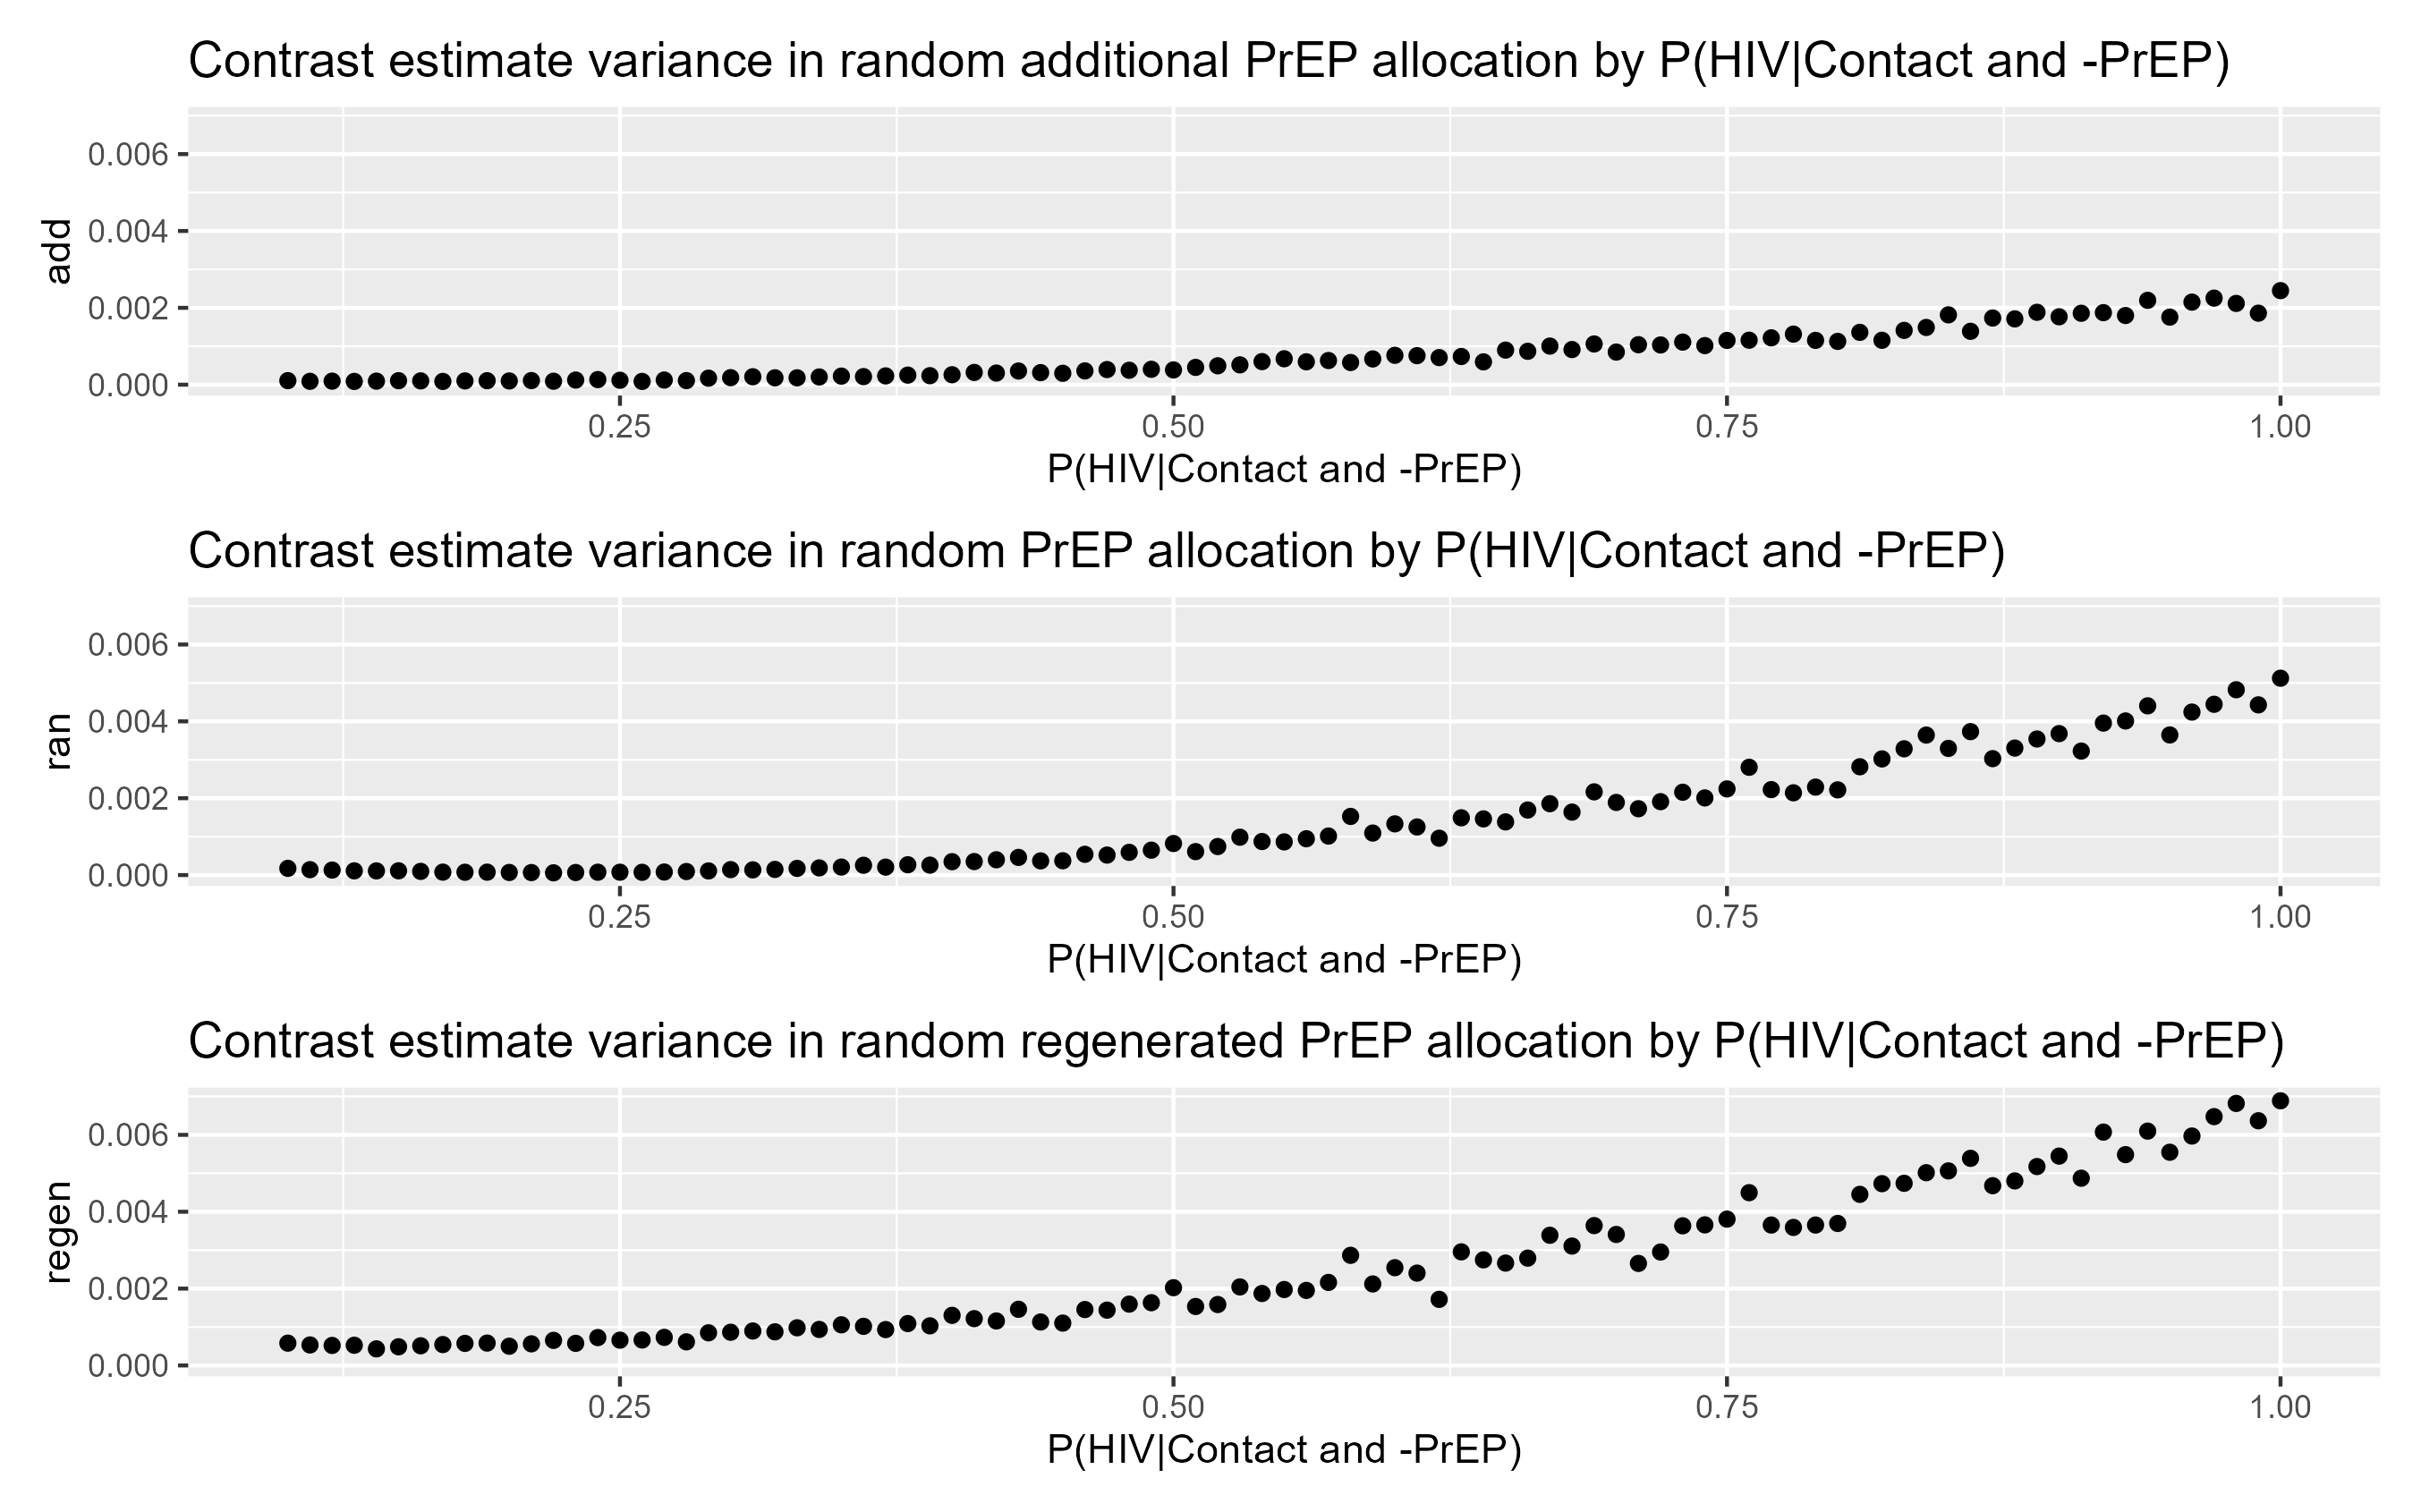
\includegraphics[scale=0.75]{Figures/p1 Variance plots.png}
    \caption{Variance of Causal Contrast estimates as $\mathbb{P}\left[\text{HIV } \vert \text{ PrEP}^{c}\right]$ increases .  From top to bottom: ``additive" Variance of Contrast of random 20\% additional vs. random 20\% PrEP allocation control, ``random" Variance of Contrast of random 40\% PrEP allocation vs. random 20\% control, ``regenerated" Variance of Contrast of random 40\% allocation on regenerated network vs. random 20\% control.}
    \label{fig:Figure 14}
\end{figure}
\subsubsection{Effect Modification by $\mathbb{P}\left[\text{HIV } \vert \text{ PrEP}\right]$}
\begin{figure}[H]
    \centering
    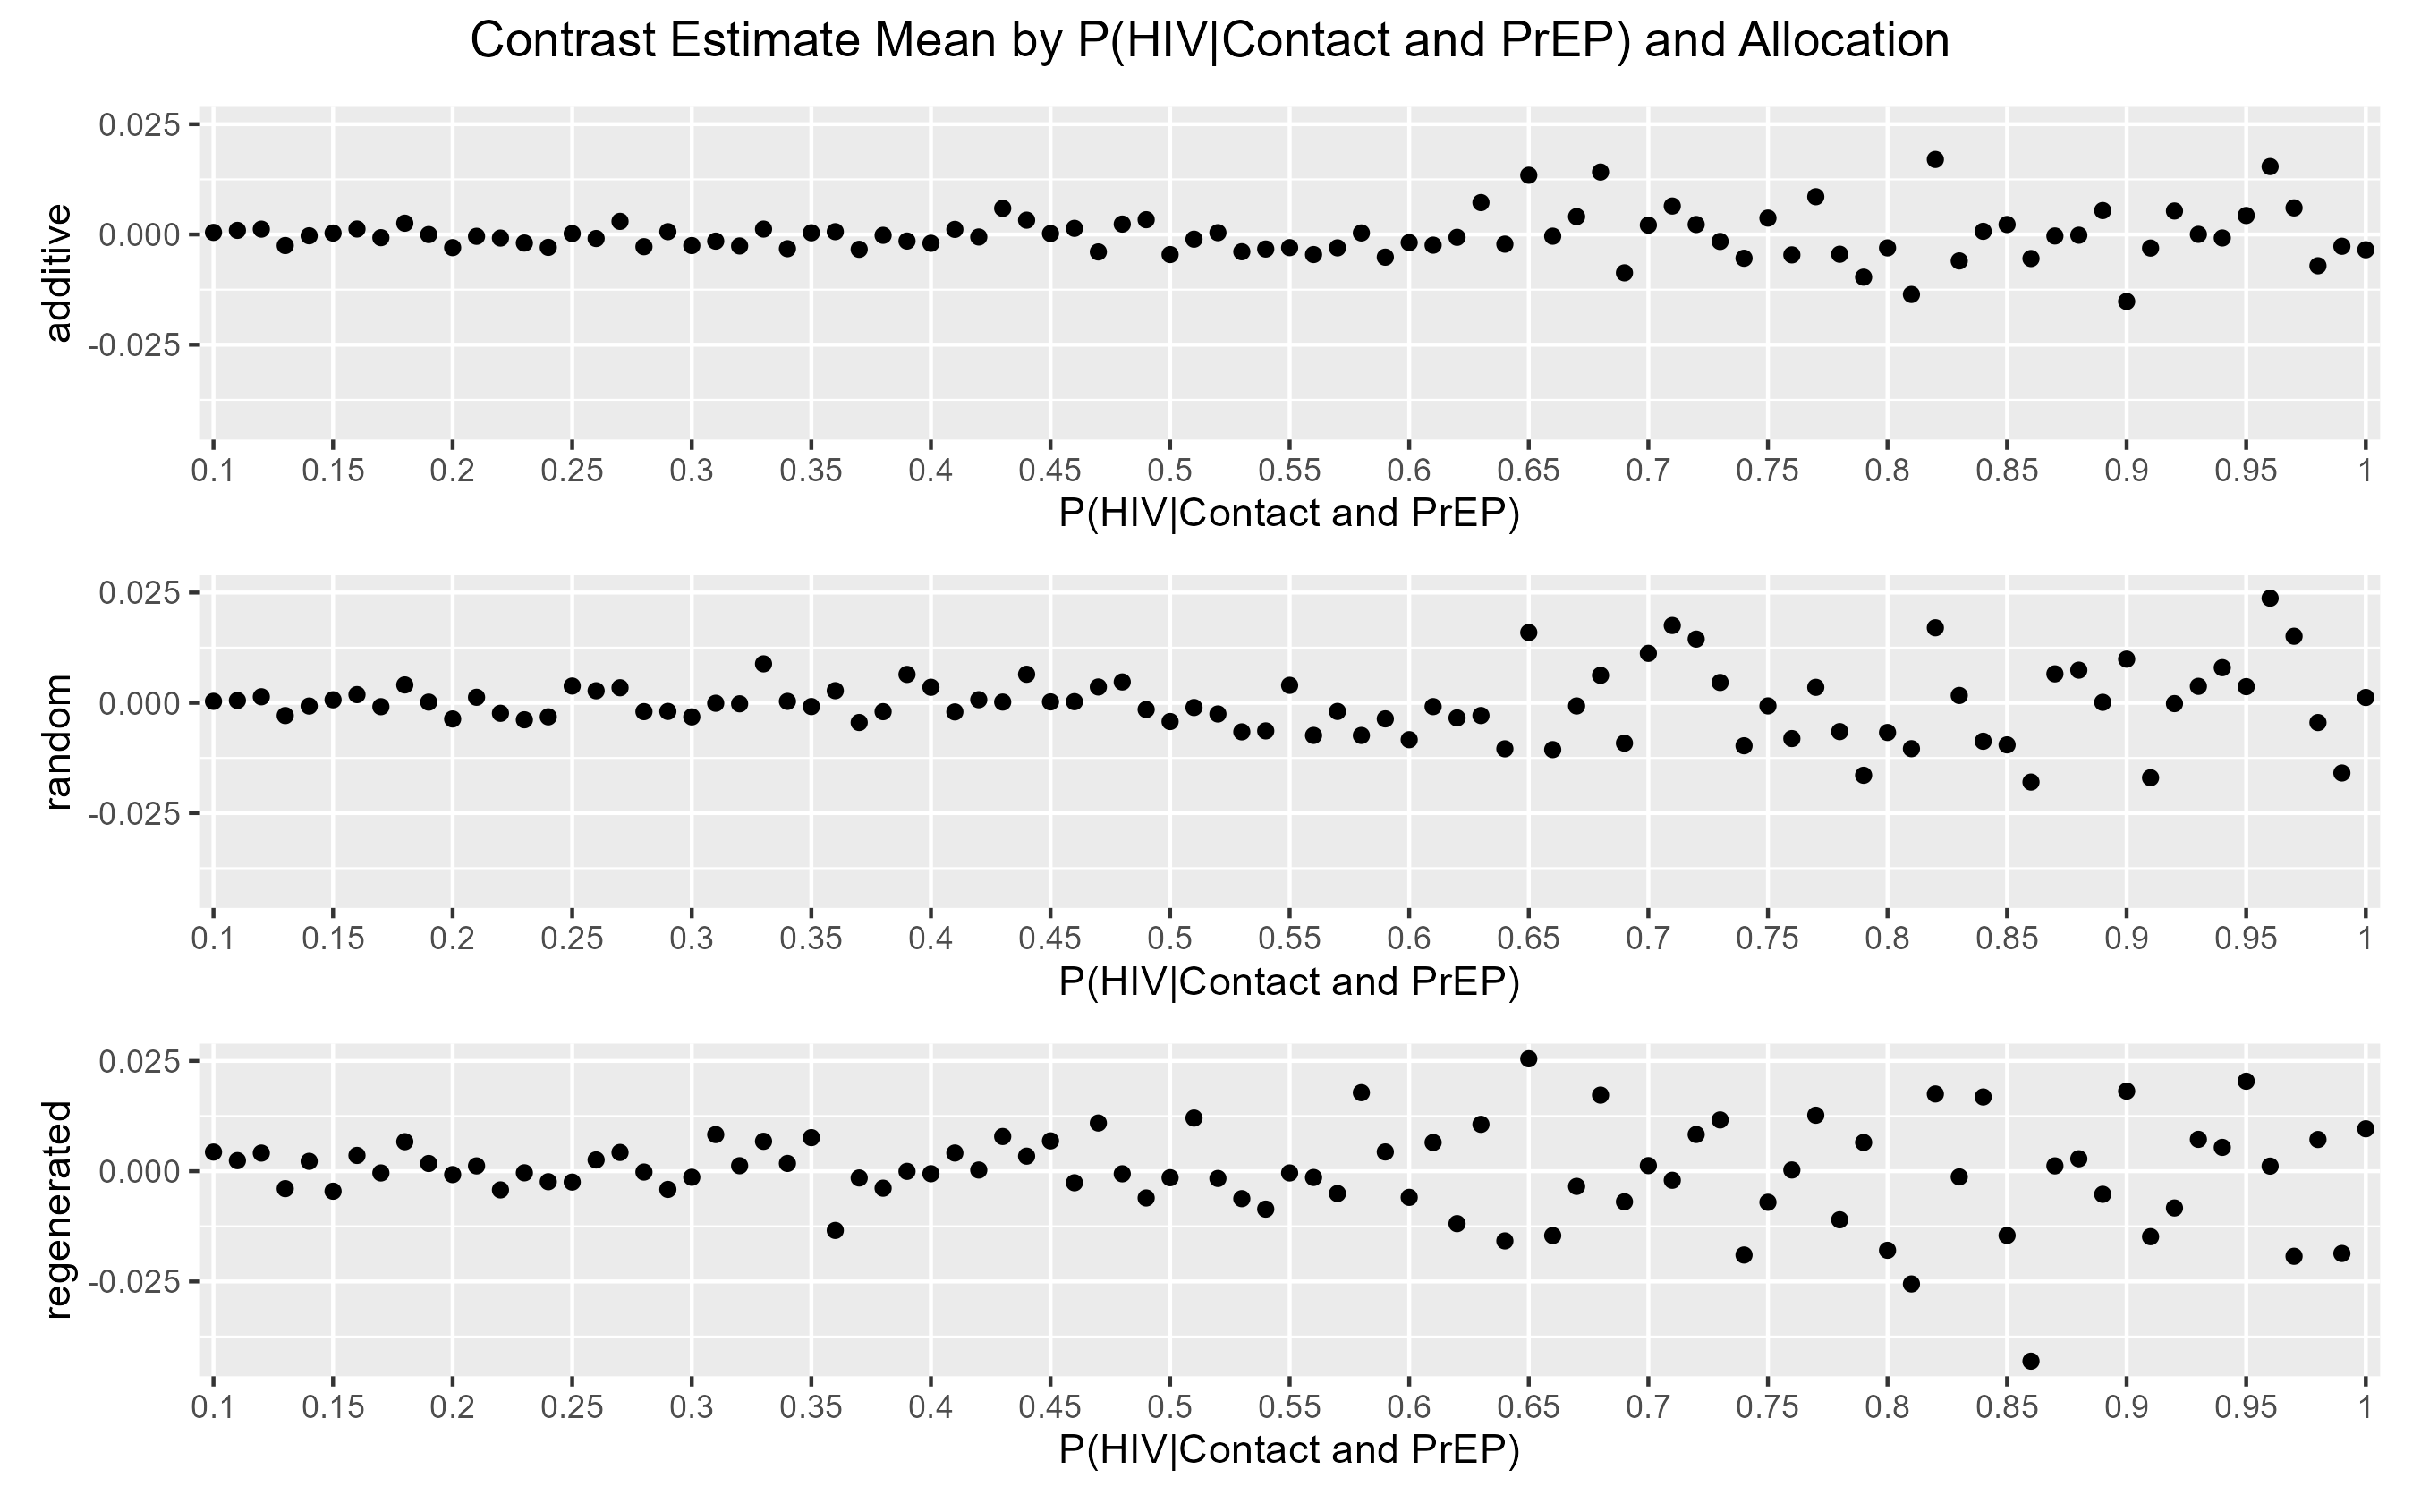
\includegraphics[scale=0.75]{Figures/p2 Mean plots.png}
    \caption{Mean Causal Contrast estimates as $\mathbb{P}\left[\text{HIV } \vert \text{ PrEP}\right]$ increases . From top to bottom: ``additive" Mean Contrast of random 20\% additional vs. random 20\% PrEP allocation control, ``random" Mean Contrast of random 40\% PrEP allocation vs. random 20\% control, ``regenerated" Mean Contrast of random 40\% allocation on regenerated network vs. random 20\% control.}
    \label{fig:Figure 15}
\end{figure}
\begin{figure}[H]
    \centering
    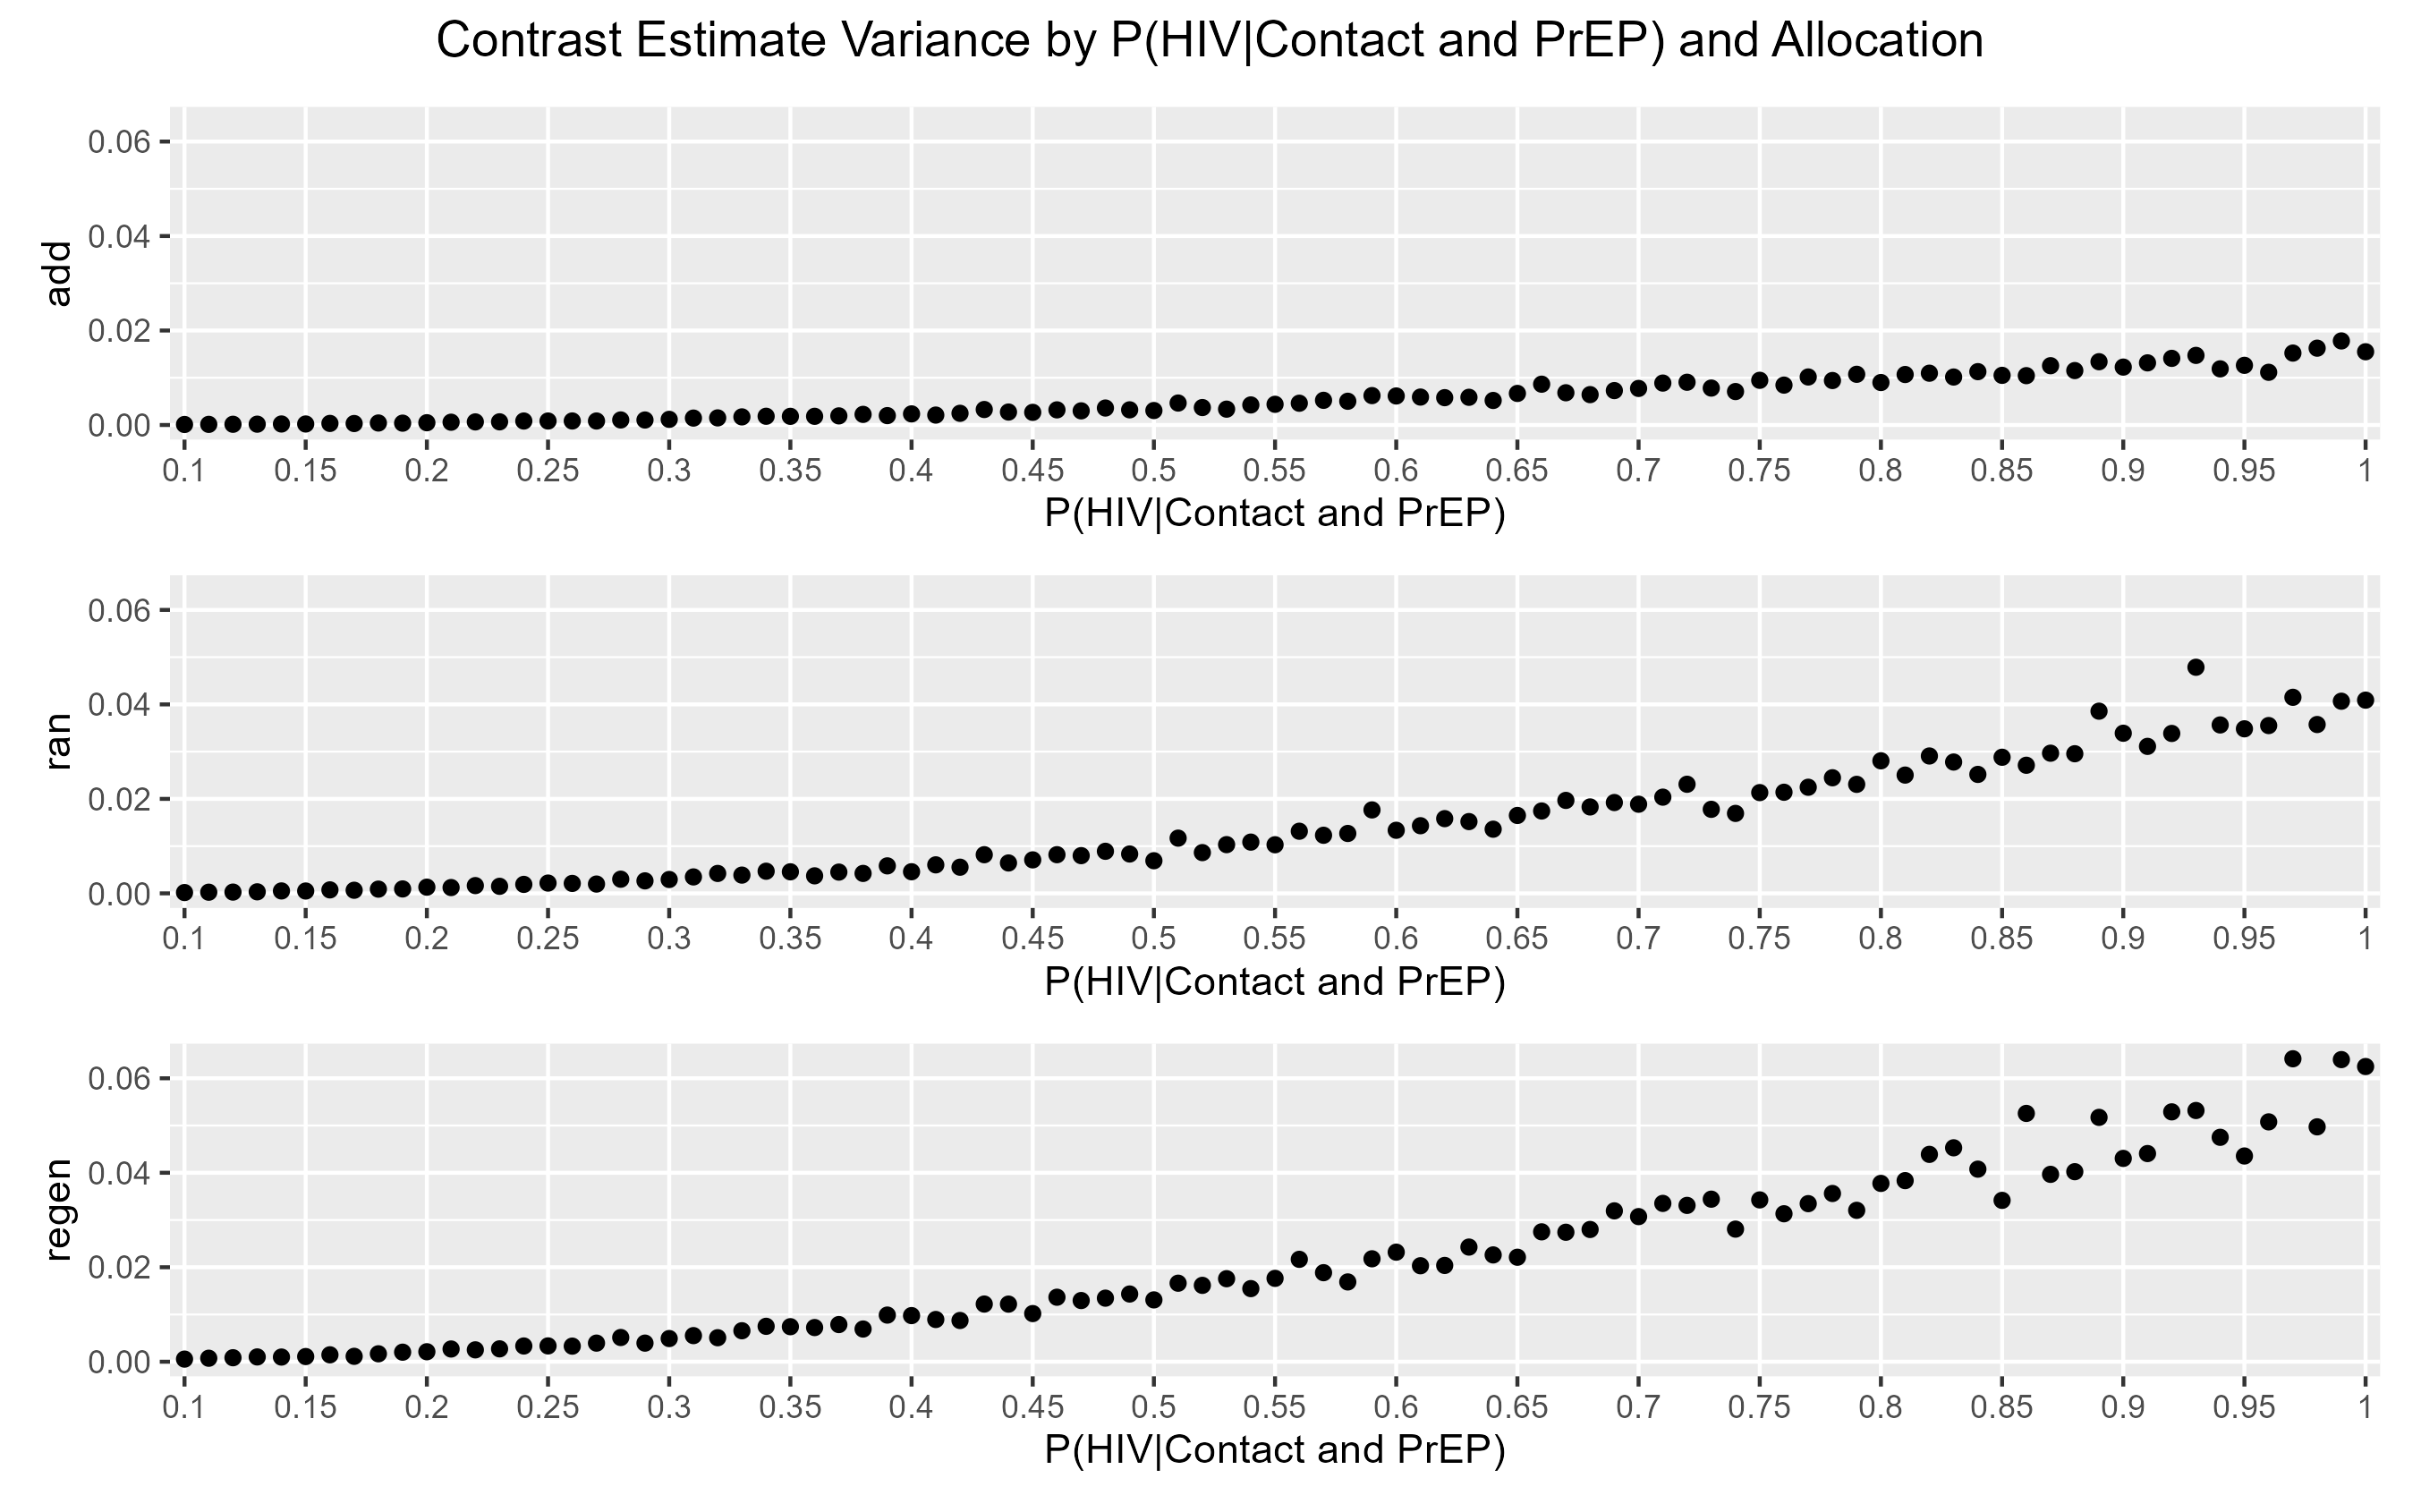
\includegraphics[scale=0.75]{Figures/p2 Variance plots.png}
    \caption{Variance of Causal Contrast estimates as $\mathbb{P}\left[\text{HIV } \vert \text{ PrEP}\right]$ increases .  From top to bottom: ``additive" Variance of Contrast of random 20\% additional vs. random 20\% PrEP allocation control, ``random" Variance of Contrast of random 40\% PrEP allocation vs. random 20\% control, ``regenerated" Variance of Contrast of random 40\% allocation on regenerated network vs. random 20\% control.}
    \label{fig:Figure 16}
\end{figure}
\subsubsection{Effect Modification by PrEP contrasts in ER model}
\begin{figure}[H]
    \centering
    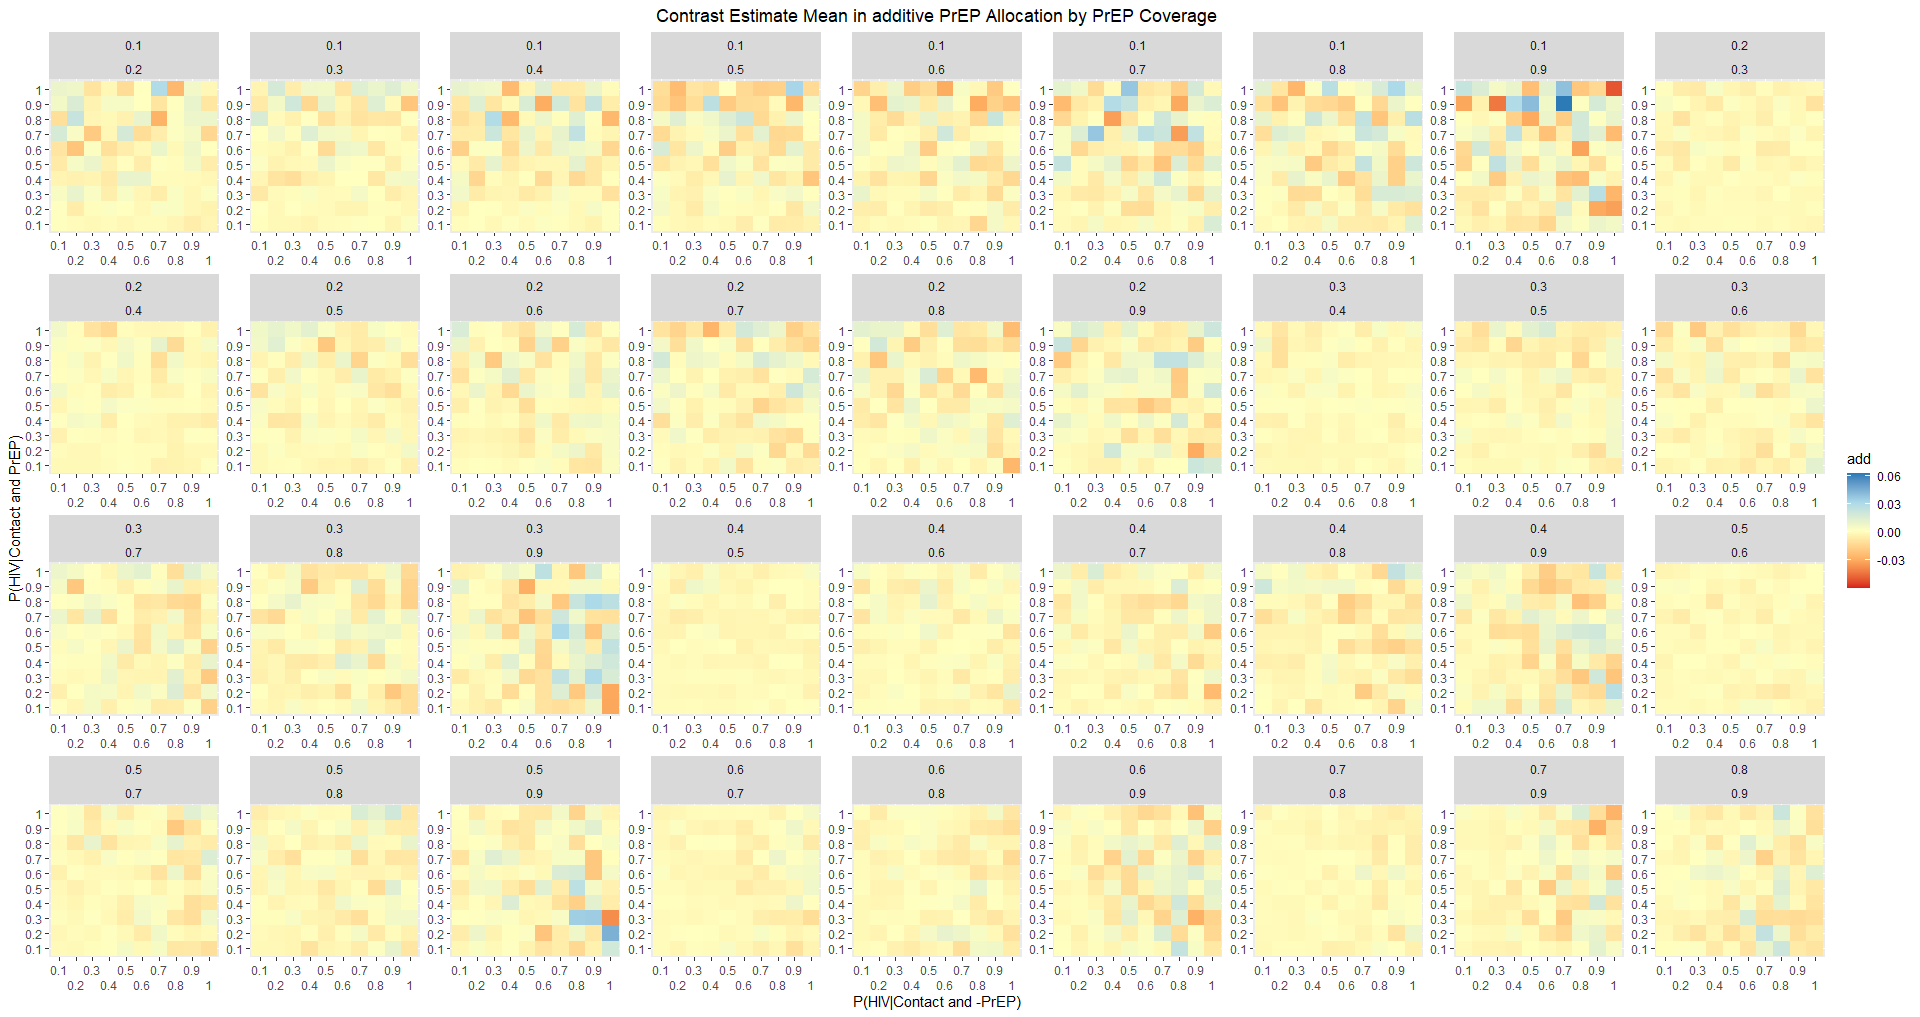
\includegraphics[scale=0.35]{Figures/PrEP Additive Mean Plots.png}
    \caption{Mean Causal Contrast estimates of random PrEP1\% additional vs. random PrEP2-PrEP1 \% PrEP allocation control. Top number indicates PrEP1/control coverage. Bottom number is PrEP2 counterfactual coverage. }
    \label{fig:Figure 17}
\end{figure}
\begin{figure}[H]
    \centering
    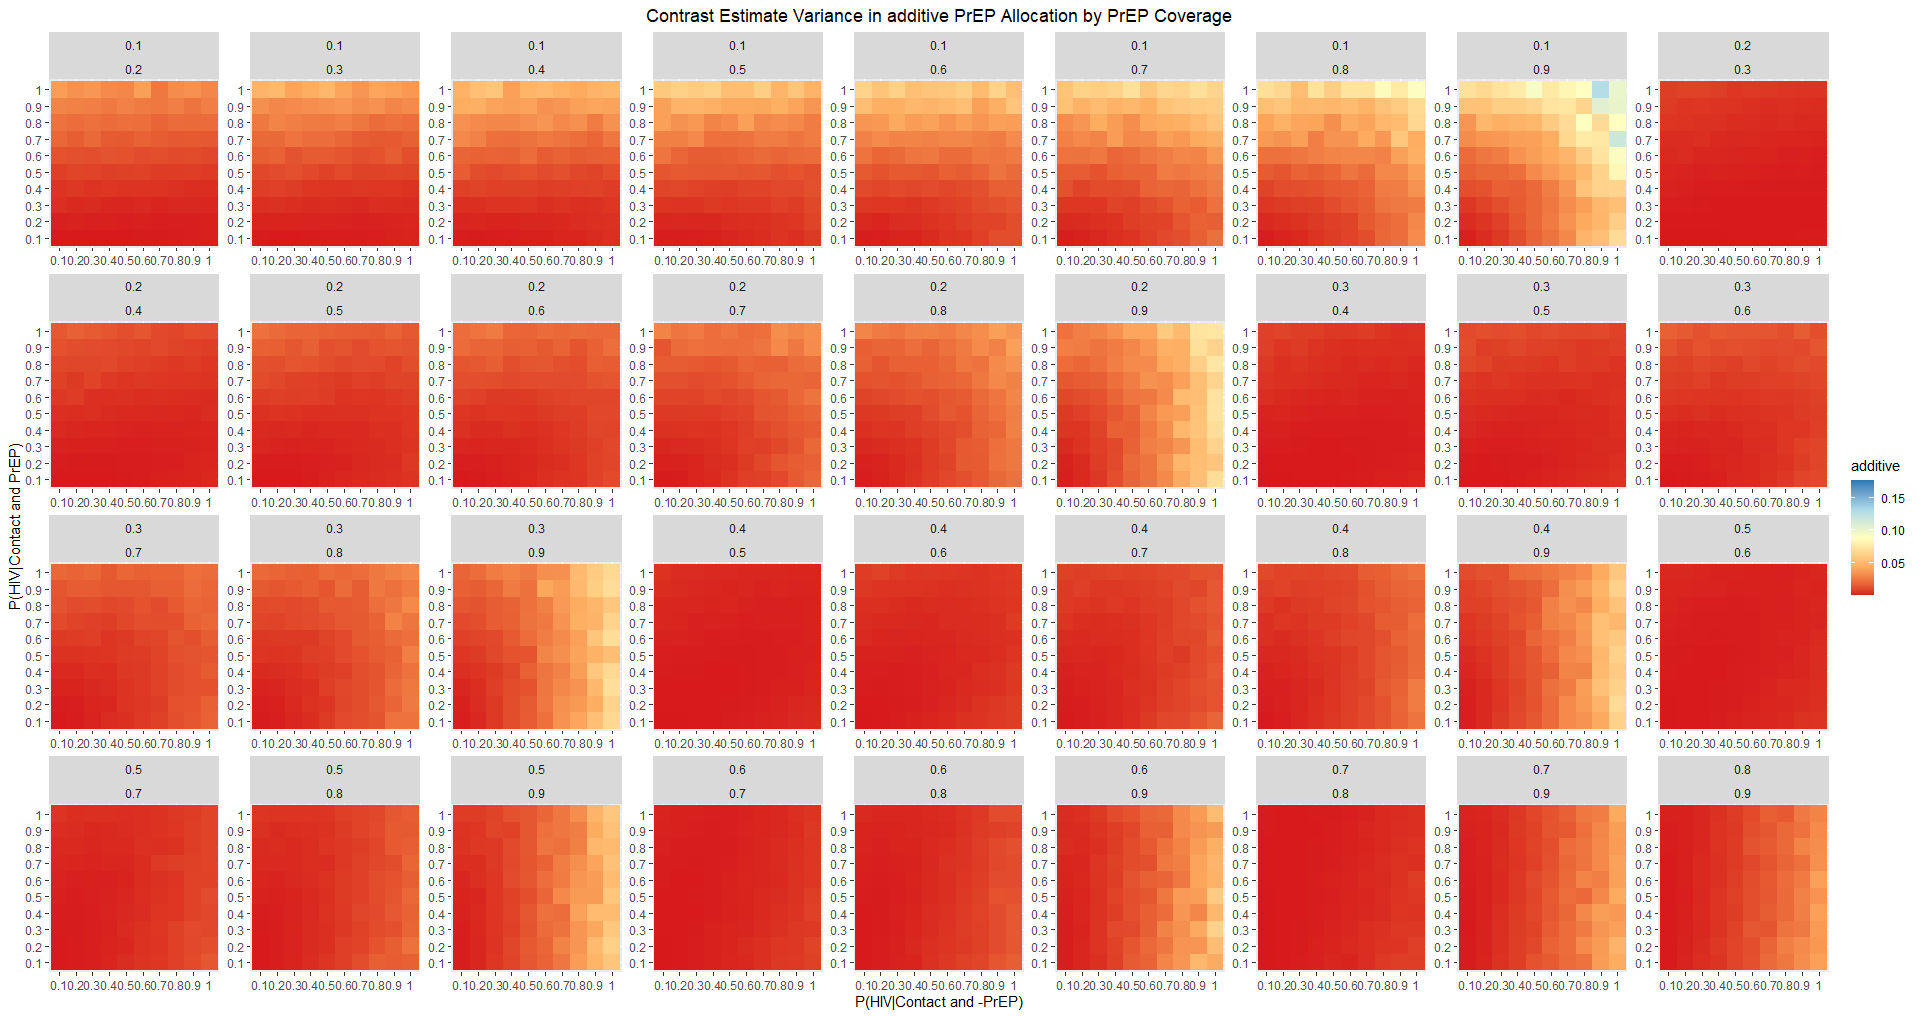
\includegraphics[scale=0.35]{Figures/PrEP Additive Variance Plots.png}
    \caption{Variance of Causal Contrast estimates of random PrEP1\% additional vs. random PrEP2-PrEP1 \% PrEP allocation control. Top number indicates PrEP1/control coverage. Bottom number is PrEP2 counterfactual coverage.}
    \label{fig:Figure 18}
\end{figure}
\begin{figure}[H]
    \centering
    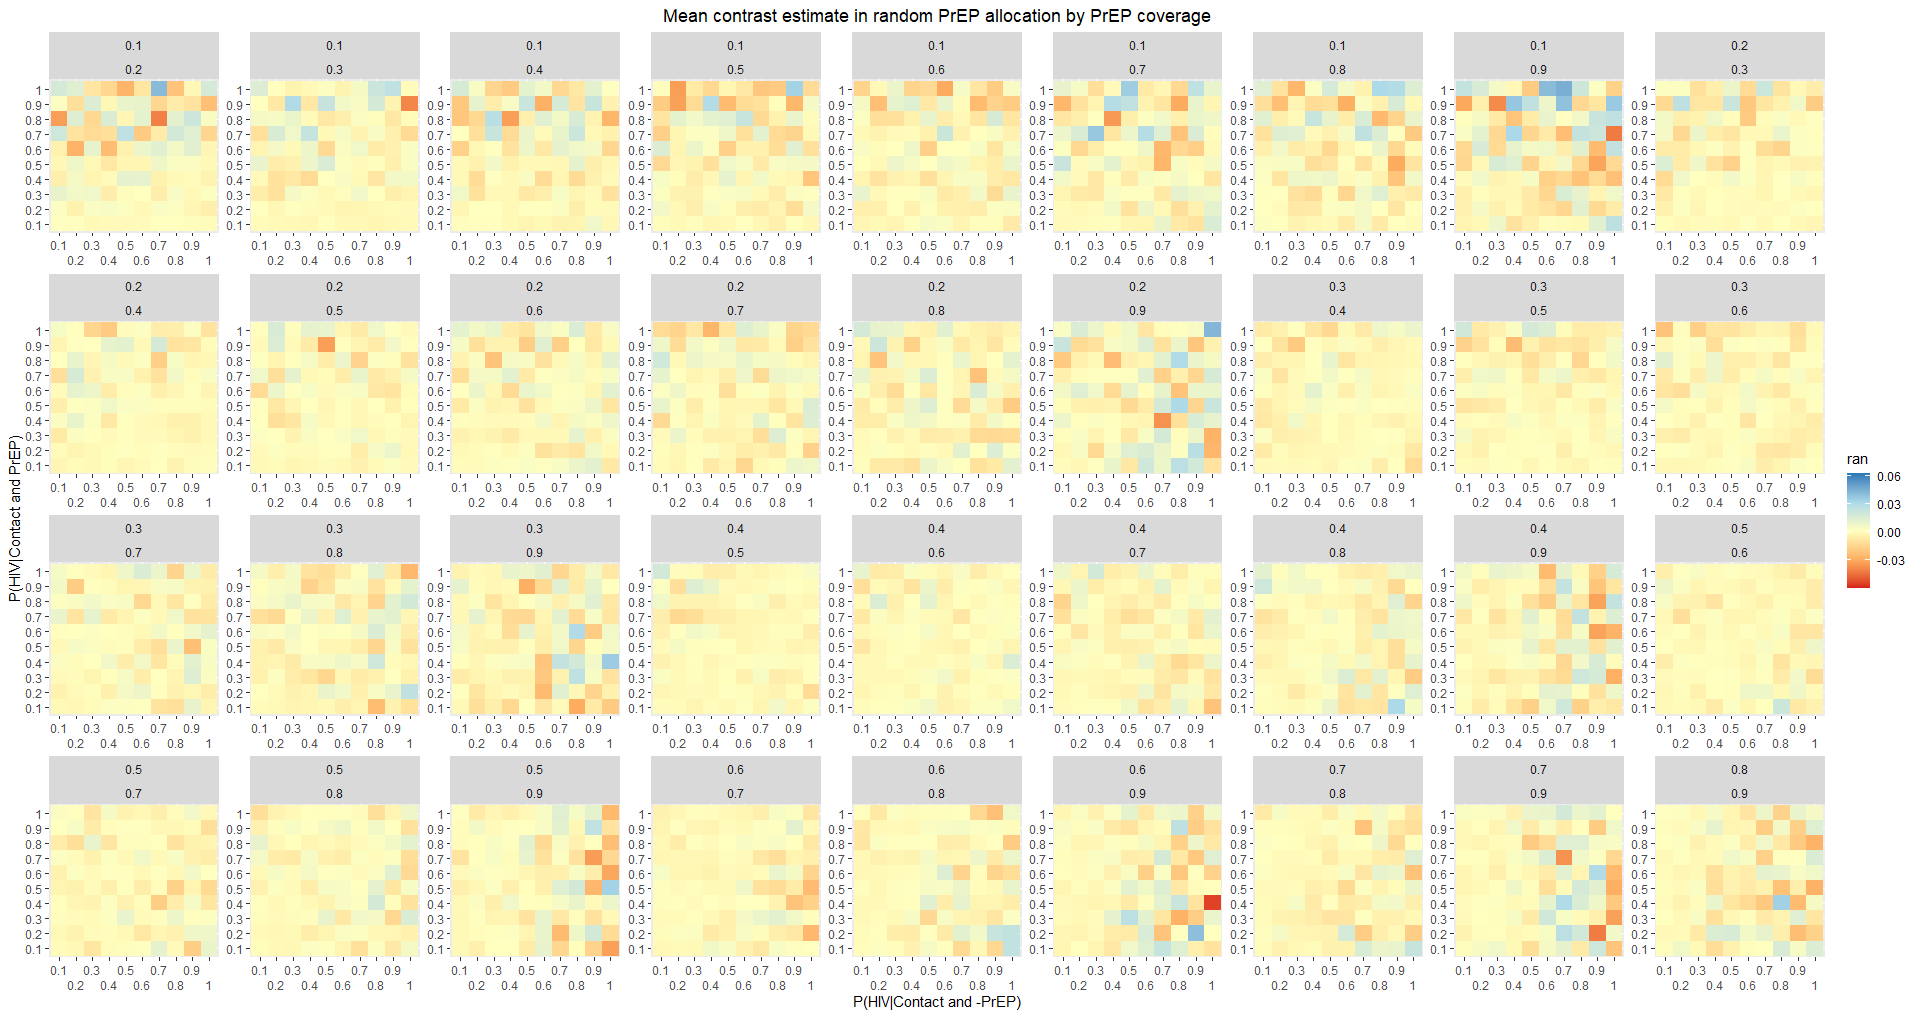
\includegraphics[scale=0.35]{Figures/PrEP Random Mean Plots.png}
    \caption{Mean Causal Contrast estimates of random PrEP1\% additional vs. random PrEP2\% PrEP allocation control. Top number indicates PrEP1/control coverage. Bottom number is PrEP2 counterfactual coverage.}
    \label{fig:Figure 19}
\end{figure}
\begin{figure}[H]
    \centering
    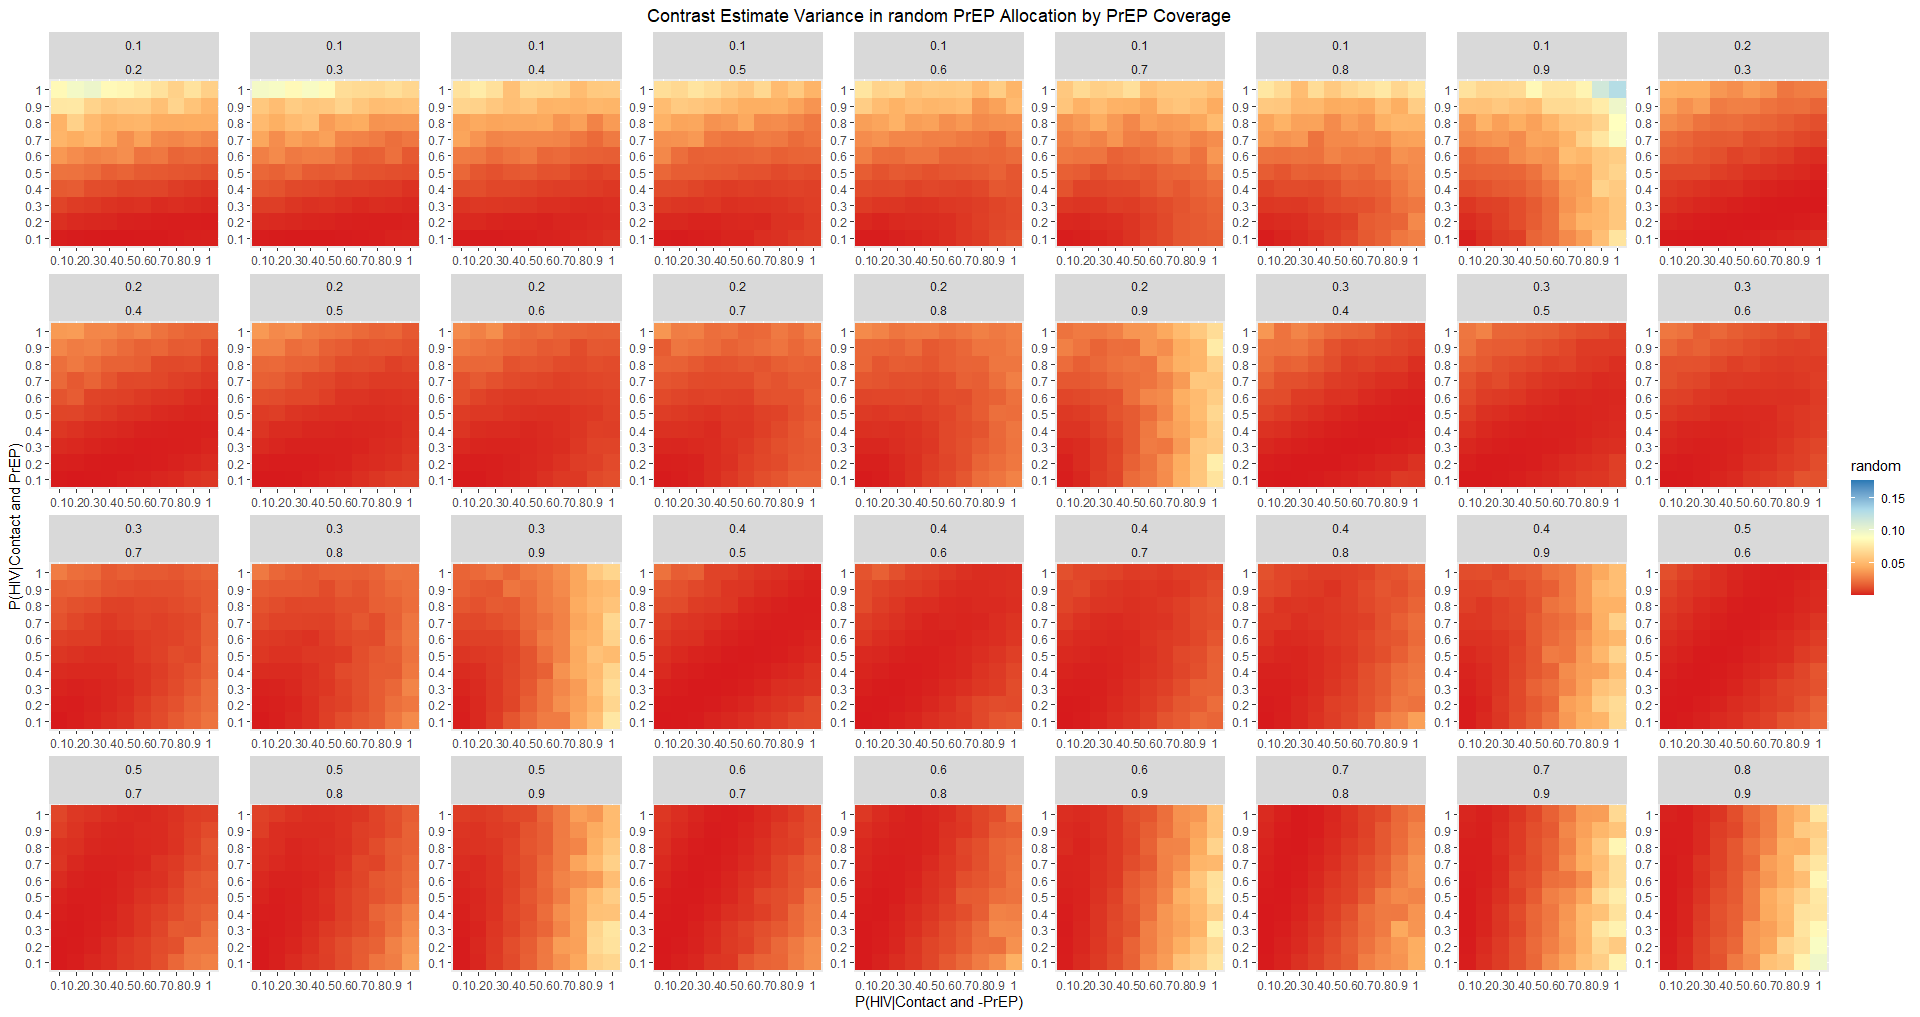
\includegraphics[scale=0.35]{Figures/PrEP Random Variance Plots.png}
    \caption{Variance of Causal Contrast estimates of random PrEP1\% additional vs. random PrEP2\% PrEP allocation control. Top number indicates PrEP1/control coverage. Bottom number is PrEP2 counterfactual coverage.}
    \label{fig:Figure 20}
\end{figure}
\begin{figure}[H]
    \centering
    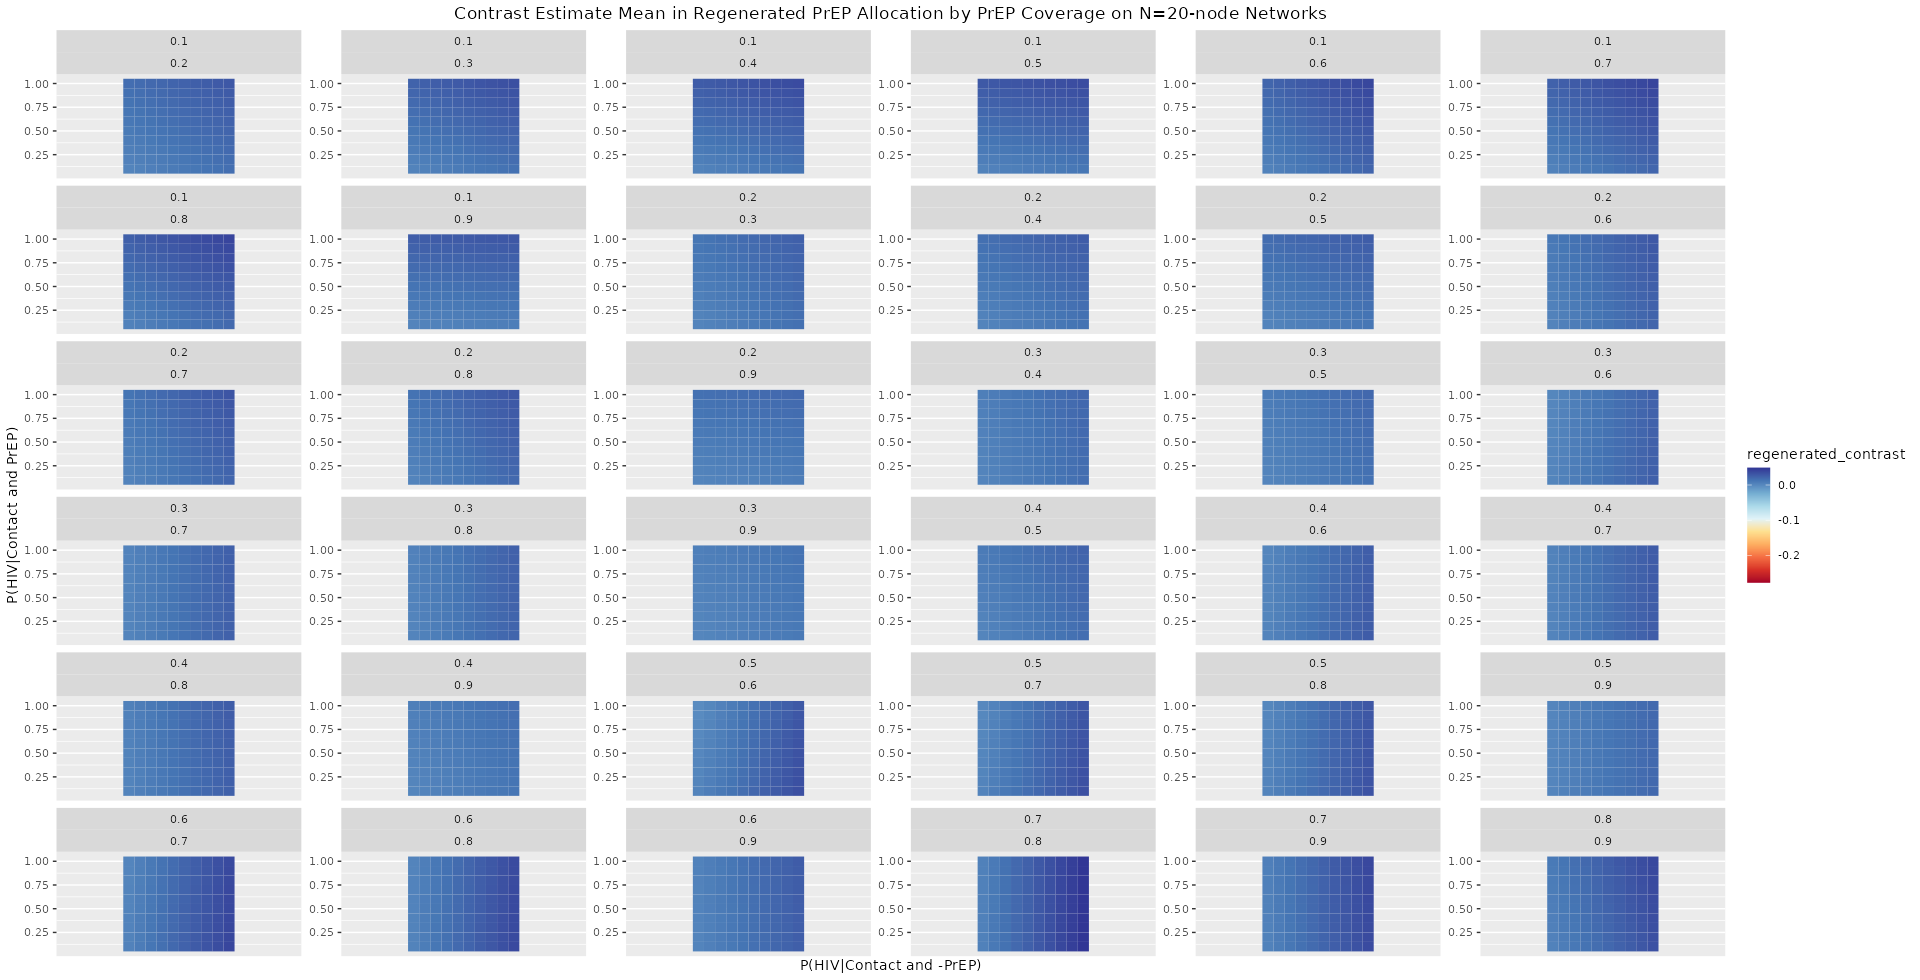
\includegraphics[scale=0.35]{Figures/PrEP Regenerated Mean Plots.png}
    \caption{Caption}
    \label{fig:Figure 21}
\end{figure}
\begin{figure}
    \centering
    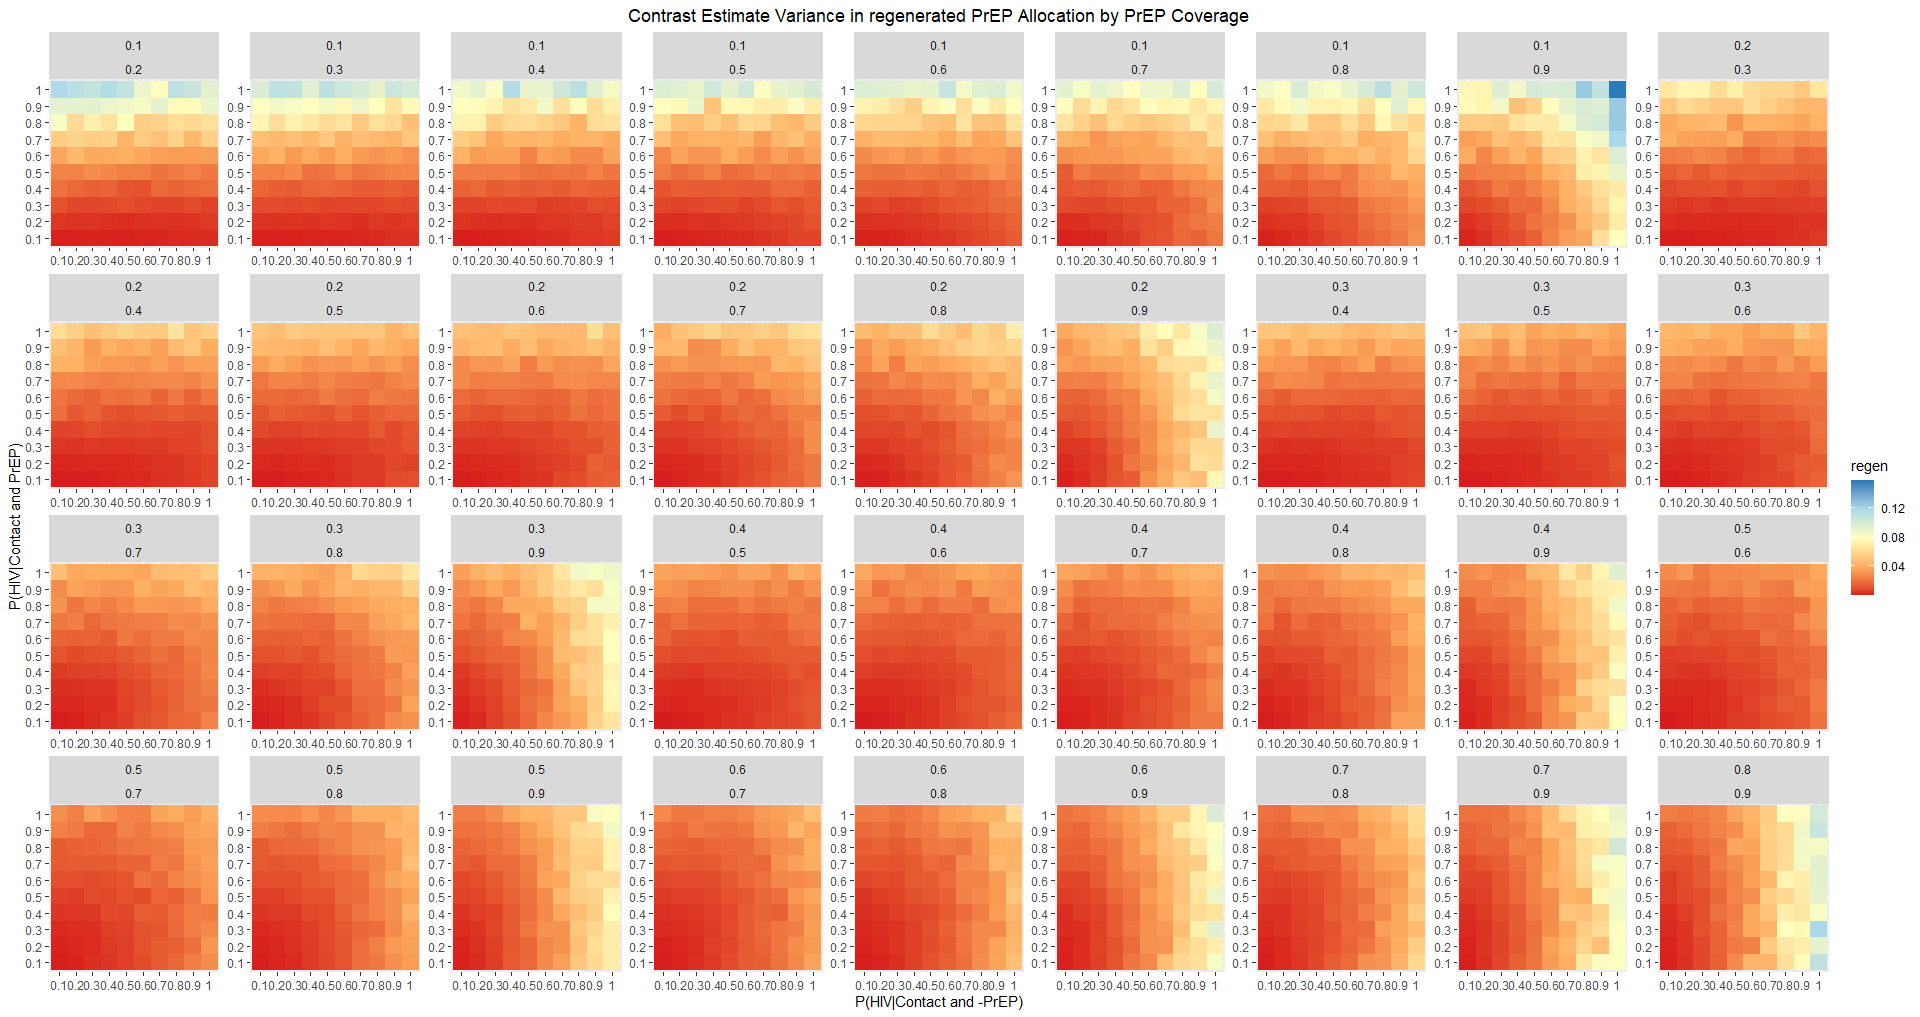
\includegraphics[scale=0.35]{Figures/PrEP Regenerated Variance Plots.png}
    \caption{Caption}
    \label{fig:Figure 22}
\end{figure}

\subsection{Other Network Models}
We also considered effect modification in two other network generating models, the Barabási–Albert scale-free graph for preferential attachment, and the Watts-Strogatz Small-World graph. The parameter values considered for these models are summarized in the table below.
\begin{center}
    \begin{tabular}{|c|c|c|}
    \hline
         Parameter & Default Value & Range Considered  \\
         \hline
         Network size $N$& 50 & Fixed \\
         \hline
         BA Preferential Attachment power ``pow" & 1 & $\left[1,2 \right]$ \\
         \hline
         WS neighborhood size ``nb" & 5 & $\Set{5,10,15,20}$ \\
         \hline
         WS rewiring probability ``rprob" & 0.05 &$\left[0.05, 0.95 \right]$ \\
         \hline
         HIV prevalence ``phiv" & 0.1 & Fixed\\
         \hline
         Control PrEP Coverage ``PrEP1" & 0.2 & Fixed\\
         \hline
         Counterfactual PrEP Coverage ``PrEP2" & 0.4 & Fixed\\
         \hline
         $\mathbb{P}\left[\text{HIV} \vert \text{PrEP}^{c}\right]$ $p1$ & 0.2 & $[0.1,1]$\\
         \hline
         $\mathbb{P}\left[\text{HIV} \vert \text{PrEP}\right]$ $p2$ & 0.1 & $[0.1,1]$\\
         \hline
         Re-sampling sample size ``nsim" & 200 & Fixed\\
         \hline
    \end{tabular}
\end{center}
\subsubsection{Effect Modification by Network Generating Model with Default Parameters}
\begin{figure}[H]
    \centering
    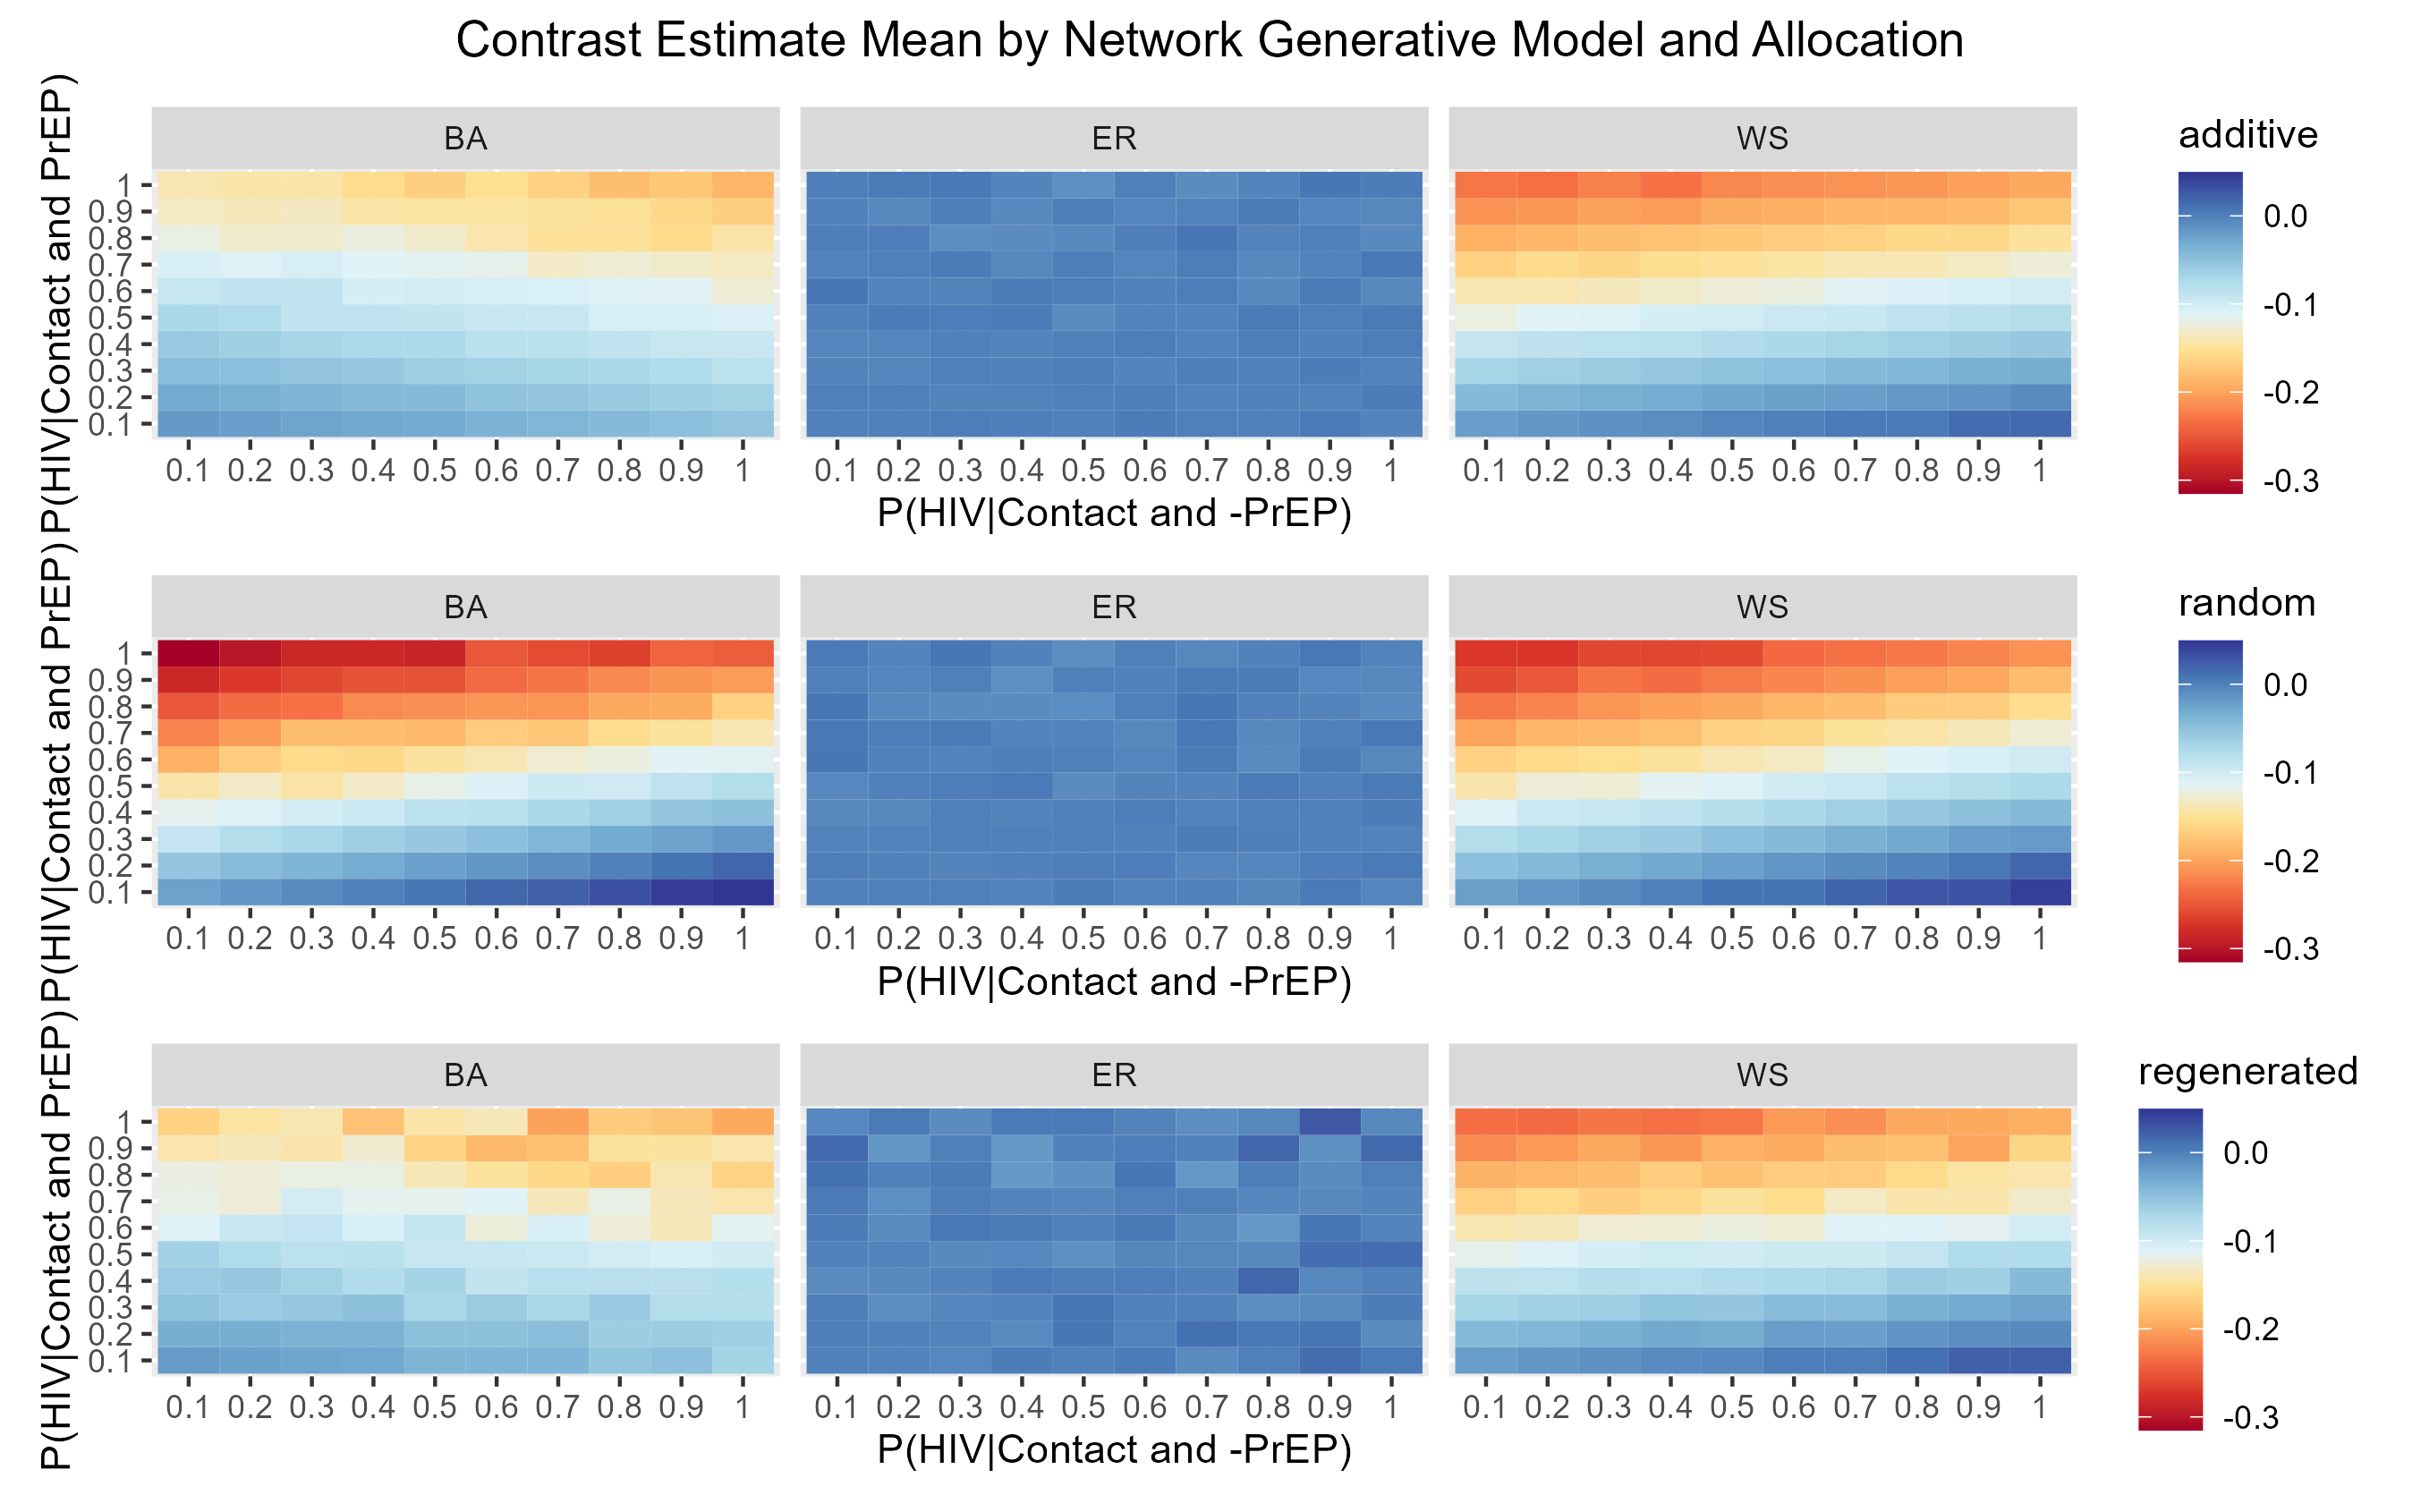
\includegraphics[scale=0.75]{Figures/Generative Model Mean plots.png}
    \caption{Mean of Causal Contrast estimates stratified by the model used to generate the networks, and by estimator. From left to right, ``BA" the Barabási–Albert scale-free model, ``ER" the Erdős–Rényi Random Graph model, ``WS" the Watts-Strogatz Small-World model. From top to bottom: ``additive" Mean Contrast of random 20\% additional vs. random 20\% PrEP allocation control, ``random" Mean Contrast of random 40\% PrEP allocation vs. random 20\% control, ``regenerated" Mean Contrast of random 40\% allocation on regenerated network vs. random 20\% control. }
    \label{fig:Figure 23}
\end{figure}
\begin{figure}[H]
    \centering
    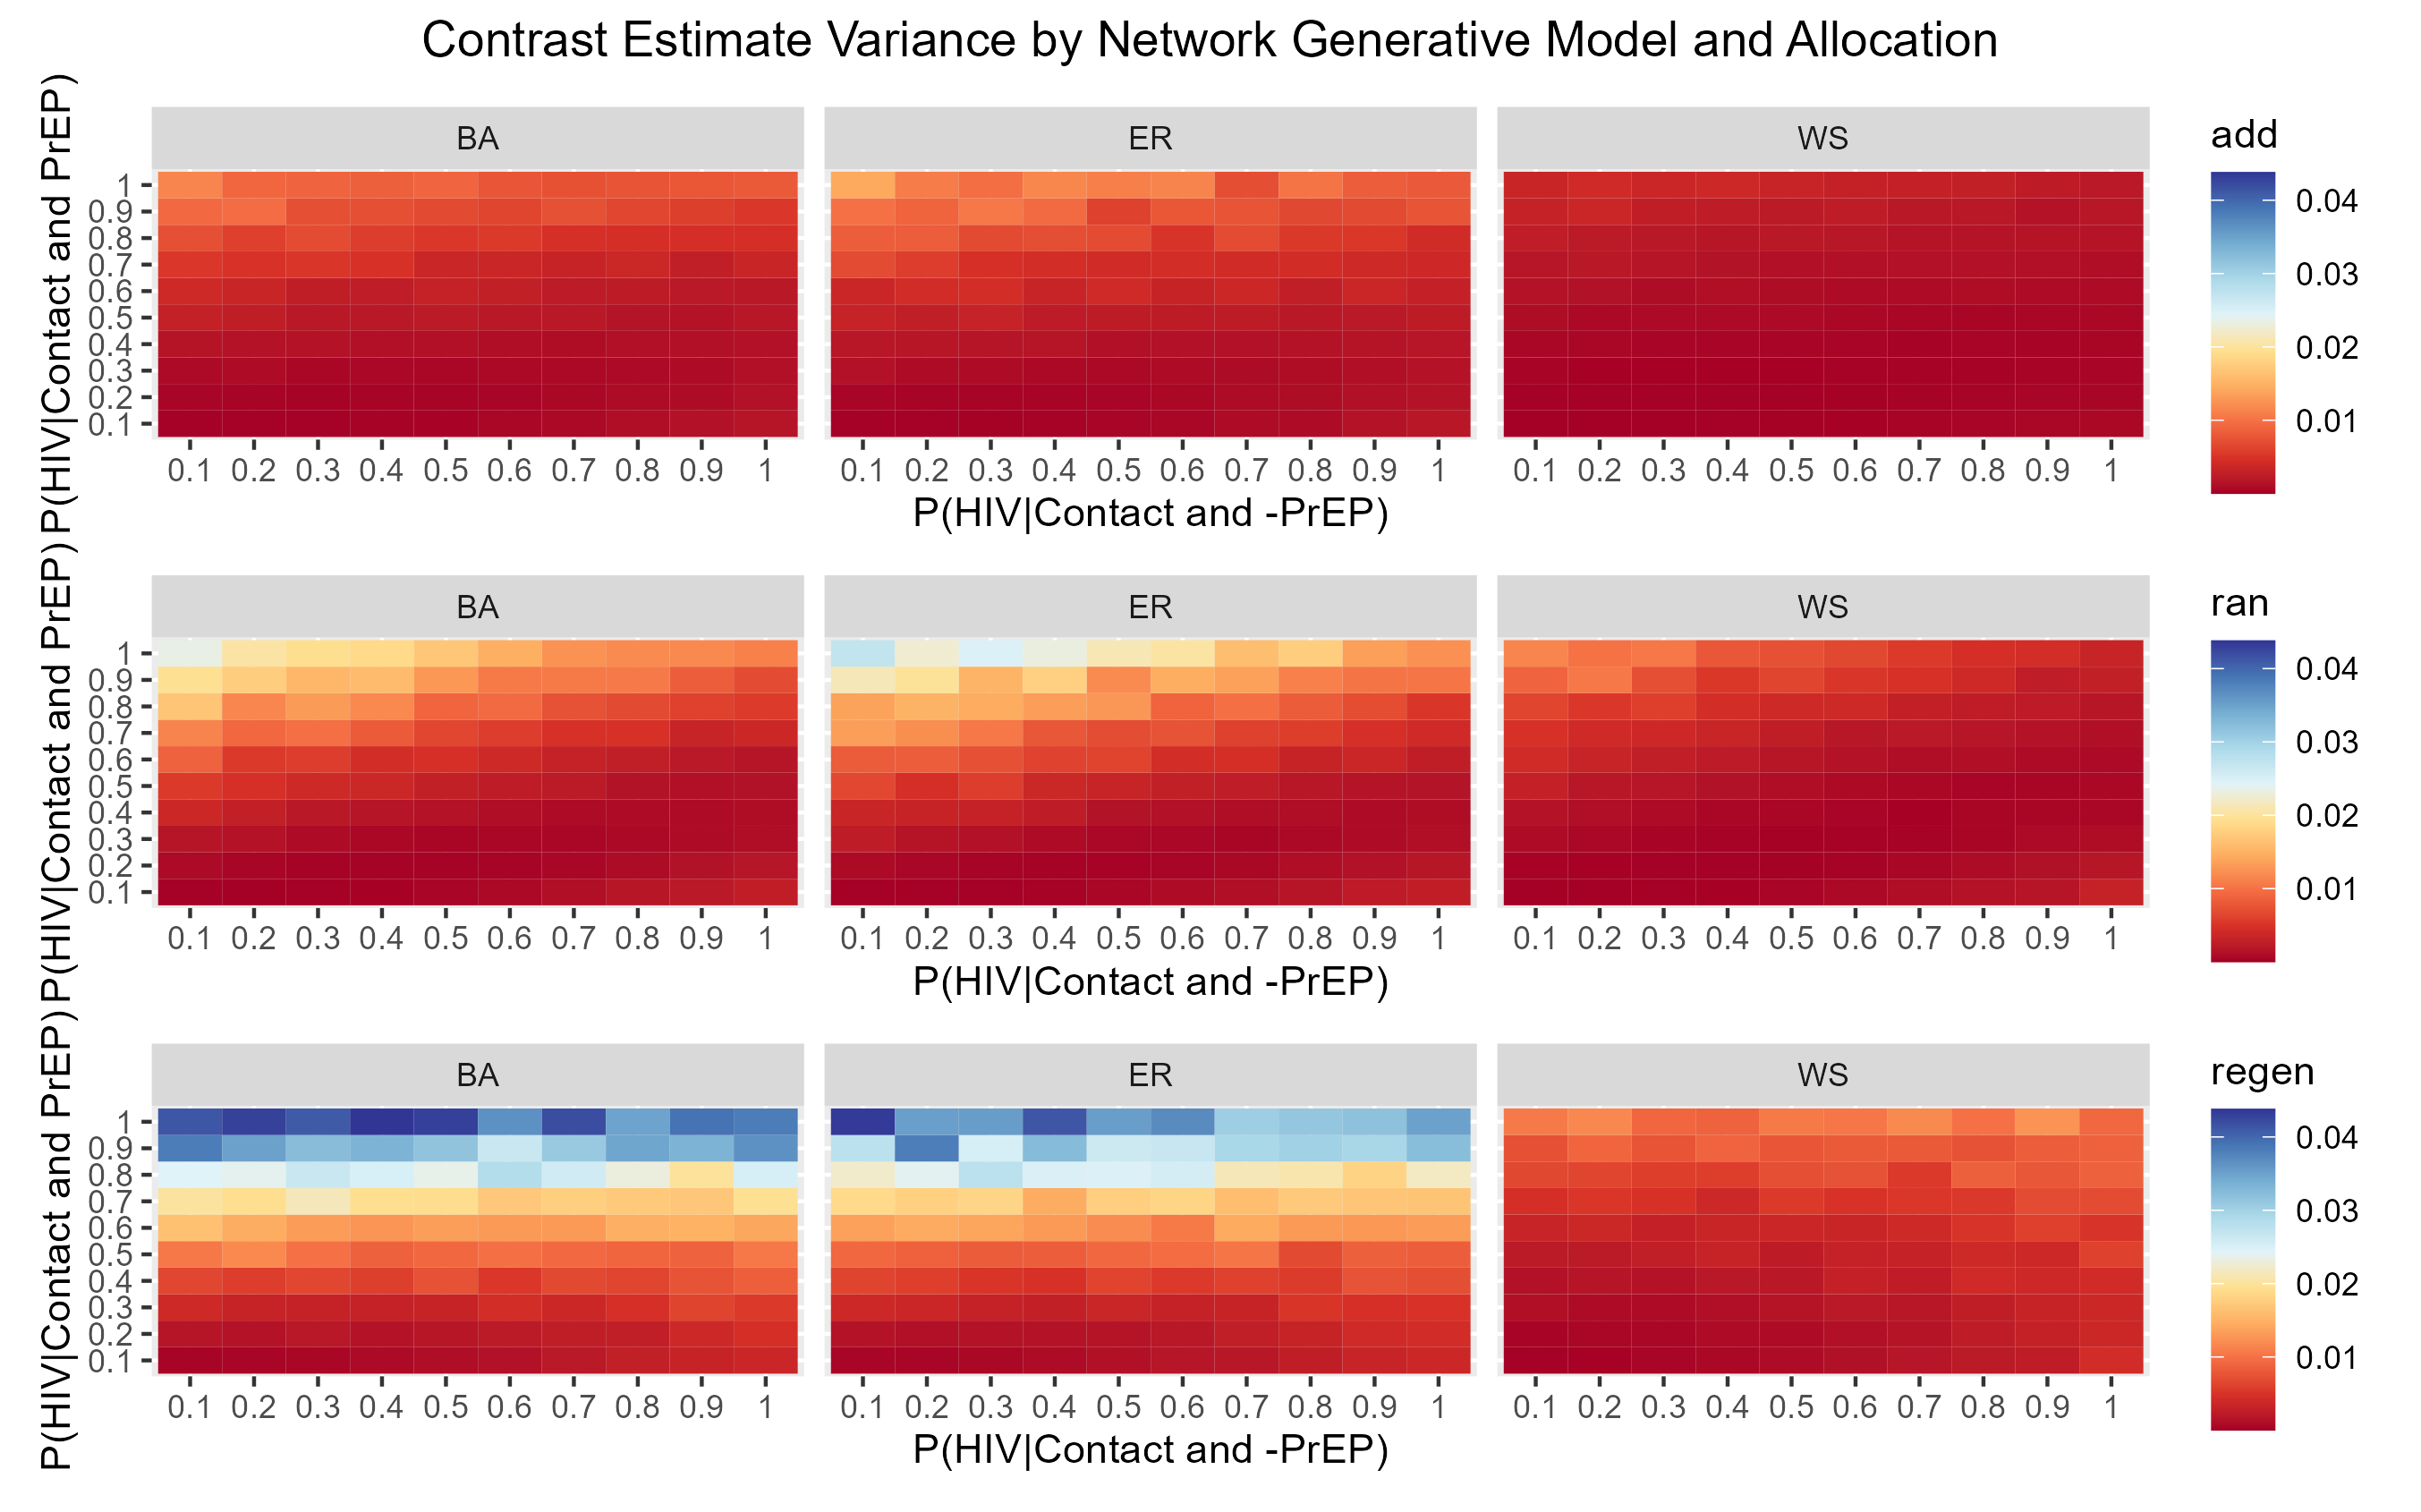
\includegraphics[scale=0.75]{Figures/Generative Model Variance plots.png}
    \caption{Variance of Causal Contrast estimates stratified by the model used to generate the networks, and by estimator. From left to right, ``BA" the Barabási–Albert scale-free model, ``ER" the Erdős–Rényi Random Graph model, ``WS" the Watts-Strogatz Small-World model. From top to bottom: ``additive" Variance of Contrast of random 20\% additional vs. random 20\% PrEP allocation control, ``random" Variance of Contrast of random 40\% PrEP allocation vs. random 20\% control, ``regenerated" Variance of Contrast of random 40\% allocation on regenerated network vs. random 20\% control.}
    \label{fig:Figure 24}
\end{figure}
\section{Appendix A}
Here we describe the details of the definition for $P$, the probability of at least one node $i$ in a network being assigned to treatment with at least one infectious contact for a given network structure $j$ and a given treatment $a$ or $a*$

Assume as before that $N$ is the network population at a given time point, that $k<N$ is the number of individuals that receive treatment, and that $n<N$ is the number of individuals with an infectious contact.

 Then, there are $\binom{N}{k}$ unique network configurations.
 
The expected number of unique network configurations in which all treated individuals have no infectious contacts (and thus a contribution of 0 to the effect estimate) is then given by $\binom{N-n}{k}$. Then, the proportion of network configurations in which at least one treated individual has at least one infectious contact is 
\begin{equation} 
\frac{{\binom{N}{k}}-{\binom{N-n}{k}}}{{\binom{N}{k}}}=1-\frac{{\binom{N-n}{k}}}{{\binom{N}{k}}}    
\end{equation}
Expanding the RHS gives:
\begin{equation}
1-\frac{\left(N-n\right)!\left(N-k\right)!}{k!\left(N-n-k\right)!}
\end{equation}
Using Stirling's Approximation as appropriate,
\begin{equation}
\approx 1-\frac{\sqrt{2\pi\left(N-n\right)}\left(\frac{N-n}{e}\right)^{N-n}\sqrt{2\pi\left(N-k\right)}\left(\frac{N-k}{e}\right)^{N-k}}{\sqrt{2\pi N}\left(\frac{N}{e}\right)^{N}\sqrt{2\pi \left(N-n-k\right)}\left(\frac{N-n-k}{e}\right)^{N-n-k}}    
\end{equation}
%see page 2b
We can then make the following approximations and simplifications:
\begin{equation}
    \frac{\sqrt{2\pi \left(N-n\right)}}{\sqrt{2\pi N}}=\sqrt{\frac{N-n}{N}}\approx 1 \text{ for } N>>n\\
    \end{equation}
    \begin{equation}
    \frac{\sqrt{2 \pi \left(N-k\right)}}{\sqrt{2 \pi \left(N-n-k\right)}}\approx 1
\end{equation}
    \begin{align}
    \frac{\left(\frac{\left(N-n\right)}{e}\right)^{N-n}}{{\left(\frac{N}{e}\right)^{N}}}&=\frac{\left(N-n\right)^{N-n}e^{N}}{N^{N}e^{N-n}}\\
     &=\frac{e^{n}}{N^{n}}\left(\frac{N-n}{N}\right)^{N-n}\\
     &=\frac{e^{n}}{N^{n}}\left(1-\frac{n}{N}\right)^{N-n}\\
     &=\frac{e^{n}}{N^{n}}\frac{\left(1-\frac{n}{N}\right)^{N}}{\left(1-\frac{n}{N}\right)^{n}}\\
     &\approx \frac{e^{n}}{N^{n}}\lim_{N \to \infty}\frac{\left(1-\frac{n}{N}\right)^{N}}{\left(1-\frac{n}{N}\right)^{n}}\\
     &=\frac{e^{n}}{N^{n}}\frac{e^{-n}}{1^{n}}\\
     &=\frac{1}{N^{n}}
\end{align}
\begin{align}
    \frac{\left(\frac{N-k}{e}\right)^{N-k}}{\left(\frac{N-n-k}{e}\right)^{N-n-k}}&\stackrel{M\coloneqq N-k}{=}\frac{\left(\frac{M}{e}\right)^{M}}{\left(\frac{M-n}{e}\right)^{M-n}}\to M^{n}\\
    \frac{M^{n}}{N^{n}}&=\left(\frac{N-k}{N}\right)^{n}
\end{align}
simplifying as appropriate gives
\begin{align}
    & \approx 1- \frac{\left(N-n\right)^{N-n}\left(N-k\right)^{N-k}}{N^{N}\left(N-n-k\right)^{N-n-k}}\\
    &= 1- N^{-N}\left(\frac{N-n}{N}\right)^{N-n}\left(N-k\right)^{n}\left(\frac{N-k}{N-n-k}\right)^{N-n-k}\\
    &=1-\left(\frac{N^{n}\left(1-\frac{n}{N}\right)^{N}\left(N-k\right)^{n}}{\left(1-\frac{n}{N}\right)^{n}}\right)\left(\frac{N-n-k}{N-k}\right)^{k+n-N}\\
    &=1-\left(\frac{N^{-n}e^{-n}\left(N-k\right)^{n}}{1}\right)\left(\frac{\left(1-\frac{n}{N-k}\right)^{n}}{\left(1-\frac{n}{N-k}\right)^{N-k}}\right)\\
    &=1-\frac{N^{-n}\left(N-k\right)^{n}e^{-n}}{e^{-n}}\\
    &=1-\frac{\left(N-k\right)^{n}}{N^{n}}\\
    &=1-\left(\frac{N-k}{N}\right)^{n}
\end{align}
\section{Appendix B: Summary Statistics by Network Model}
\end{document}